\documentclass[12pt,a4paper,oneside]{report}
\usepackage[spanish]{babel}
\selectlanguage{spanish}
\usepackage{times}
\usepackage{graphicx,color}
\usepackage{xcolor}
\usepackage[utf8]{inputenc}
\usepackage[T1]{fontenc}
\usepackage{verbatim}
\usepackage{longtable}
\usepackage{tabularx} % Para tablas de mas de una página
\usepackage{multirow}
\usepackage{multicol}
\usepackage[refpages]{gloss}
\usepackage{float}
\usepackage{anysize}
\usepackage{appendix}
%\usepackage{listings}
\usepackage{latexsym}
\usepackage{amsmath}
\usepackage{amssymb}

\usepackage{algorithm}
\usepackage{algorithmicx}
\usepackage{algpseudocode}

% Terminología española para los algoritmos (algorithm / algpseudocode).
\floatname{algorithm}{Algoritmo}
\algrenewcommand\algorithmicrequire{\textbf{Datos:}}
\algrenewcommand\algorithmicensure{\textbf{Resultado:}}
\algrenewcommand\algorithmicend{\textbf{fin}}
\algrenewcommand\algorithmicdo{\textbf{hacer}}
\algrenewcommand\algorithmicfor{\textbf{para}}
\algrenewcommand\algorithmicforall{\textbf{para todo}}
\algrenewcommand\algorithmicwhile{\textbf{mientras}}
\algrenewcommand\algorithmicloop{\textbf{bucle}}
\algrenewcommand\algorithmicif{\textbf{si}}
\algrenewcommand\algorithmicthen{\textbf{entonces}}
\algrenewcommand\algorithmicelse{\textbf{si no}}
\algrenewcommand\algorithmicfunction{\textbf{función}}
\algrenewcommand\algorithmicprocedure{\textbf{procedimiento}}
\algrenewcommand\algorithmicreturn{\textbf{devolver}}

\usepackage{hyperref}

\usepackage{listings}
\usepackage{listingsutf8} % habilita inputencoding en listings
\lstset{
  inputencoding=utf8,
  basicstyle=\ttfamily\small,
  columns=fullflexible,
  keepspaces=true,
  upquote=true,
  % Mapeo de acentos para listings:
  literate=
   {á}{{\'a}}1 {é}{{\'e}}1 {í}{{\'\i}}1 {ó}{{\'o}}1 {ú}{{\'u}}1
   {Á}{{\'A}}1 {É}{{\'E}}1 {Í}{{\'I}}1 {Ó}{{\'O}}1 {Ú}{{\'U}}1
   {ñ}{{\~n}}1 {Ñ}{{\~N}}1 {ü}{{\"u}}1 {Ü}{{\"U}}1
}
\usepackage{setspace}
\usepackage{ragged2e}
\usepackage{xcolor}
\usepackage{tikz}
\usetikzlibrary{shapes, positioning, arrows.meta, calc, shapes.geometric, arrows, decorations.pathreplacing}

%New colors defined below
\definecolor{codegreen}{rgb}{0,0.6,0}
\definecolor{codegray}{rgb}{0.5,0.5,0.5}
\definecolor{codepurple}{rgb}{0.58,0,0.82}
\definecolor{backcolour}{rgb}{0.95,0.95,0.92}

%Code listing style named "mystyle"
\lstdefinestyle{mystyle}{
  backgroundcolor=\color{backcolour}, 
  commentstyle=\color{codegreen},
  keywordstyle=\color{magenta},
  numberstyle=\tiny\color{codegray},
  stringstyle=\color{codepurple},
  basicstyle=\ttfamily\footnotesize,
  breakatwhitespace=false,         
  breaklines=true,                 
  captionpos=b,                    
  keepspaces=true,                 
  numbers=left,                    
  numbersep=5pt,                  
  showspaces=false,                
  showstringspaces=false,
  showtabs=false,                  
  tabsize=2
}

%"mystyle" code listing set
\lstset{style=mystyle}


% -------- Entornos de teoremas y macros de normas --------
\usepackage{amsthm}
\newtheorem{teorema}{Teorema}[chapter]
\newtheorem{lema}[teorema]{Lema}
\newtheorem{proposicion}[teorema]{Proposición}
\newtheorem{corolario}[teorema]{Corolario}
\newtheorem{definicion}[teorema]{Definición}
\newtheorem{suposicion}[teorema]{Hipótesis}
\newtheorem{observacion}[teorema]{Observación}
\newtheorem{remark}[teorema]{Remark}

% Macros útiles
\newcommand{\R}{\mathbb{R}}
\newcommand{\E}{\mathbb{E}}
\newcommand{\Emp}{\widehat{\mathbb{E}}}
\newcommand{\Prob}{\mathbb{P}}
\newcommand{\norm}[1]{\left\lVert #1 \right\rVert}
\newcommand{\abs}[1]{\left\lvert #1 \right\rvert}
\newcommand{\Holder}[3]{\left[ #1 \right]_{#2; #3}}
\newcommand{\Loss}{\mathcal{J}} % para la función de pérdida


\newcommand{\autor}{Nombre del autor}

\newcommand{\titulo}{Título de la tesis}

\newcommand{\asesor}{Nombre del asesor}

\renewcommand*{\contentsname}{Tabla de contenidos}
\renewcommand*{\listtablename}{Índice de tablas}
\renewcommand*{\listfigurename}{Índice de figuras}
\renewcommand{\baselinestretch}{1.0}
\renewcommand{\appendixname}{Anexos}
\renewcommand{\appendixtocname}{Anexos}
\renewcommand{\appendixpagename}{Anexos}
\renewcommand{\thetable}{\arabic{chapter}.\arabic{table}}
\renewcommand*{\tablename}{Tabla}
\renewcommand*{\chaptername}{Capítulo}
\renewcommand*{\thechapter}{\Roman{chapter}}
\renewcommand{\thesection}{\arabic{chapter}.\arabic{section}}
\renewcommand{\figurename}{Figura}
\renewcommand{\thefigure}{\arabic{chapter}.\arabic{figure}}
\renewcommand{\theequation}{\arabic{chapter}.\arabic{equation}}

\renewcommand\bibname{Bibliografía}

\begin{document}
%----------------------------------------------------------------------------------------
%	CONFIGURACION
%----------------------------------------------------------------------------------------
\marginsize{3.0cm}{3.0cm}{3.0cm}{3.0cm}

\begin{titlepage}

\begin{center}
{\Large \bf PONTIFICIA UNIVERSIDAD CATÓLICA DEL PERÚ}\\
\vspace{8mm} 
{\Large \bf ESCUELA DE POSGRADO}\\
\vspace{1cm}

\includegraphics[height=3.5cm]{imagenes/logo_pucp.png}
\vspace{1cm}

{\Large \normalfont \bfseries Análisis de Convergencia de Soluciones de EDPs con Redes Neuronales PINN: Caso de la Ecuación de Poisson 2D}\\ 
\vspace{1cm}

{\bf Tesis para optar el grado académico de Magíster en \\
Matemática Aplicada}\\
\vspace{2cm}

{\bf AUTOR}\\[0.5cm]
{\large Michael Hurtado Enríquez}\\
\vspace{2cm}

{\bf ASESOR}\\[0.5 cm] 
{\large MSc. Xyoby Chávez}\\
\vspace{2cm}

{Lima, \today}
\end{center}
\end{titlepage}
\pagenumbering{roman}
%-----------------
%	Resumen
%-----------------

\chapter*{\centering \large Resumen}
\addcontentsline{toc}{chapter}{Resumen}
\markboth{Resumen}{Resumen}

Esta tesis estudia la convergencia de aproximaciones de la ecuación de Poisson mediante redes neuronales físicamente informadas (PINNs), con énfasis en la relación entre la pérdida residual y el error de solución. Se reconstruye el marco de Shin, Darbon y Karniadakis para problemas elípticos, precisando las hipótesis de regularidad, muestreo y estabilidad, y se estudia una extensión condicional con comparadores y minimizadores aproximados, cuyas tolerancias deben estar controladas por la escala del peso regularizador. El análisis distingue las garantías referidas a minimizadores globales de los resultados obtenidos mediante optimización numérica finita. Se estudian problemas unidimensionales, se examina la reproducción de experimentos de referencia y se resuelve Poisson en dos dimensiones con condiciones de Dirichlet impuestas mediante penalización o mediante una parametrización que las satisface exactamente. Para el problema bidimensional se realizan veinticuatro entrenamientos, correspondientes a cuatro resoluciones, tres semillas y dos tratamientos de frontera. En la resolución más alta, la mediana del error relativo $L^2$ disminuye de $6.19\times10^{-3}$ a $1.74\times10^{-4}$ al utilizar Dirichlet fuerte. La evaluación independiente de residuos y errores muestra, además, que una pérdida reducida en los puntos de colocación puede coexistir con residuos mayores fuera de ellos. La reproducción del caso oscilatorio presenta discrepancias que no se atribuyen a una causa única. Un estudio adicional con redes $\tanh$ de dos capas ocultas distingue continuación de la optimización (A), anchura con muestreo fijo (B) y escalamiento conjunto de muestras y anchura (C). La pérdida residual disminuye, pero en C la pendiente log--log descriptiva ($-0.284$, tres escalas) es menos pronunciada que la escala suficiente de referencia ($-0.750$); el presupuesto de optimización no es proporcional al tamaño de muestra. Los resultados respaldan la utilidad de imponer exactamente las condiciones de frontera en el problema estudiado, pero no constituyen una verificación de las hipótesis asintóticas ni una comparación general de superioridad frente a los métodos de elementos y volúmenes finitos.

\noindent\textbf{Palabras clave:} redes neuronales físicamente informadas, ecuación de Poisson, convergencia, condiciones de Dirichlet, error residual.

\clearpage
\chapter*{\centering \large Abstract}
\addcontentsline{toc}{chapter}{Abstract}
\markboth{Abstract}{Abstract}

This thesis studies the convergence of approximations to the Poisson equation using physics-informed neural networks (PINNs), with particular attention to the relationship between residual loss and solution error. The convergence framework of Shin, Darbon, and Karniadakis for elliptic problems is reconstructed, making explicit the regularity, sampling, and stability assumptions required to relate an empirical loss to functional error estimates. A conditional extension admitting approximate comparators and approximately optimal solutions is examined, subject to quantitative tolerances on the scale of the regularization weight. The analysis distinguishes theoretical guarantees for global minimizers from results produced by finite numerical optimization. One-dimensional problems are examined, reference experiments are revisited, and the two-dimensional Poisson equation is solved with Dirichlet conditions imposed either by a penalty or by a parameterization that satisfies them exactly. For the two-dimensional problem, twenty-four training runs are performed using four resolutions, three random seeds, and two boundary treatments. At the finest resolution, the median relative $L^2$ error decreases from $6\mathord{.}19\times10^{-3}$ to $1\mathord{.}74\times10^{-4}$ when strong Dirichlet enforcement is used. Independent evaluations of residuals and errors also reveal that small losses at collocation points may coexist with substantially larger residuals away from those points. The oscillatory reference example exhibits discrepancies that cannot be assigned to a single established cause. Additional experiments with two-hidden-layer $\tanh$ networks distinguish optimization continuation (A), width variation with fixed samples (B), and joint sample--width scaling (C). Although residual losses decrease, the descriptive log--log slope in C ($-0.284$, three scales) is shallower than the sufficient reference exponent ($-0.750$); the optimization budget does not scale proportionally with sample count. These findings support the usefulness of exactly imposing boundary conditions in the problem studied, but they do not verify the asymptotic assumptions of the convergence theorems or establish general superiority over finite element or finite volume methods.

\noindent\textbf{Keywords:} physics-informed neural networks, Poisson equation, convergence, Dirichlet boundary conditions, residual error.


%-------------------------
%	Agradecimientos
%-----------------------

\chapter*{\centering \large Agradecimientos} % No numerado y centrado
\addcontentsline{toc}{chapter}{Agradecimientos}
\markboth{Agradecimientos}{Agradecimientos}

\justify
Agradezco profundamente a mi madre y a mi novia por su incondicional apoyo y comprensión a lo largo de este proceso. Sus palabras de aliento y su presencia constante han sido fundamentales para alcanzar este logro. También quiero expresar mi más sincero agradecimiento a mi asesor, el MSc. Xyoby Chávez, por su invaluable orientación y confianza. Su constante apoyo y su fe en mi capacidad para abordar este tema han sido esenciales para culminar con éxito esta etapa de mi carrera.


%--------------------------
%	TABLA DE CONTENIDOS
%--------------------------
\cleardoublepage
\addcontentsline{toc}{chapter}{\contentsname}
\tableofcontents \newpage

\addcontentsline{toc}{chapter}{\listfigurename}
\listoffigures \newpage

%\addcontentsline{toc}{chapter}{\listtablename}
%\listoftables \newpage
\makegloss
\newpage
\pagenumbering{arabic}

%-----------------
%	Capítulo 1
%-----------------
\doublespacing

\chapter*{Introducción}
\addcontentsline{toc}{chapter}{Introducción}
\markboth{Introducción}{Introducción}

Las ecuaciones diferenciales parciales (EDPs) elípticas aparecen de manera natural en numerosos problemas de la física, la ingeniería y las ciencias aplicadas, como la electrostática, la difusión de calor o la mecánica de fluidos. Dentro de esta familia, la ecuación de Poisson ocupa un lugar central por su amplia aplicabilidad y por ser un modelo prototípico para el estudio de métodos analíticos y numéricos. Tradicionalmente, su solución se ha abordado mediante esquemas de diferencias finitas~\cite{leveque2007}, elementos finitos~\cite{strang1973, babuska1994} o volúmenes finitos, cuya teoría está bien establecida pero que pueden enfrentar limitaciones en geometrías complejas o en altas dimensiones.

Las \emph{redes neuronales físicamente informadas} (\emph{Physics-Informed Neural Networks}, PINNs) representan la solución mediante una red y entrenan sus parámetros penalizando el residuo de la ecuación y el defecto de frontera. Esta formulación, desarrollada entre otros por Raissi et al.~\cite{raissi2017physics, raissi2019}, permite incorporar también observaciones interiores. Entre los antecedentes del uso de redes neuronales para aproximar soluciones de EDPs se encuentran Dissanayake y Phan-Thien (1994)~\cite{dissanayake1994neural} y, posteriormente, Lagaris et al. (1998)~\cite{lagaris1998artificial}; las arquitecturas y técnicas de entrenamiento actuales se apoyan en avances posteriores del aprendizaje profundo~\cite{goodfellow2016deep, lecun2015deep}.

Una pérdida residual pequeña en un conjunto finito de puntos no asegura, por sí sola, que el residuo sea pequeño en todo el dominio. Tampoco garantiza que el optimizador encuentre un minimizador con las propiedades requeridas por los resultados de convergencia. Estas dos dificultades motivan el estudio matemático y los experimentos de esta tesis.

La motivación específica de este trabajo es doble. Por un lado, se busca contar con un marco matemático que permita justificar, bajo hipótesis claras, la convergencia de las PINNs hacia la solución exacta de una EDP elíptica, tanto en normas débiles como fuertes. Por otro lado, se pretende contrastar estos resultados teóricos con experimentos numéricos concretos para la ecuación de Poisson en una y dos dimensiones, analizando el comportamiento de los errores y comparando el desempeño de las PINNs con métodos clásicos.

La tesis se organiza en cuatro capítulos de desarrollo y uno de conclusiones. En el capítulo I, dedicado a los preliminares matemáticos, se introduce el marco analítico necesario basándose en la teoría clásica de EDPs elípticas~\cite{gilbarg2001elliptic}: definición de operadores lineales, formulación del problema de Dirichlet, espacios de Hölder, espacios $L^2$ y de Sobolev, principio del máximo, celdas de Voronoi y el teorema de existencia de Schauder. Estos elementos se utilizarán posteriormente para formular y probar los resultados de convergencia.

En el capítulo II, dedicado a las redes neuronales, se presentan las nociones básicas de redes neuronales artificiales~\cite{bishop2006pattern} y se describe la construcción de las PINNs. Se detallan las funciones de activación, el algoritmo de optimización Adam~\cite{adam2015method}, el uso de diferenciación automática y la formulación de la función de pérdida, así como una versión regularizada adecuada para problemas elípticos.

El capítulo III, dedicado al análisis de convergencia, constituye el núcleo teórico de la tesis. Siguiendo la línea de trabajo de Shin et al.~\cite{shin2020convergence}, se establecen lemas, hipótesis y teoremas que describen las condiciones bajo las cuales una familia de redes neuronales minimizadoras de la pérdida PINN converge hacia la solución clásica de la ecuación de Poisson. Se analizan tanto la convergencia en la norma $C^0(U)$ como el paso a normas más fuertes, como $H^1(U)$, apoyándose en construcciones basadas en celdas de Voronoi.

Finalmente, en el capítulo IV, dedicado a los resultados computacionales, se implementan y estudian numéricamente distintas configuraciones de PINNs aplicadas a problemas de Poisson 1D y 2D. Se presentan curvas de error en normas $L^2$ y $H^1$ en función del número de puntos de entrenamiento, comparando una PINN estándar, una penalización cuadrática media y la regularización discreta LIPR. Se examinan además los dos problemas unidimensionales de Shin et al., junto con un diagnóstico numérico de regularidad H\"older y cobertura. Por último, se comparan los resultados para Poisson 2D con métodos de elementos finitos y volúmenes finitos, dejando explícitas las diferencias entre presupuestos de cómputo y procedimientos de discretización.




\chapter{Preliminares matem\'aticos}

\section{Introducci\'on}

Las ecuaciones diferenciales parciales (EDPs) constituyen una herramienta central para modelar fenómenos físicos, biológicos y de ingeniería. Dentro de la clase de ecuaciones elípticas, la ecuación de Poisson ocupa un lugar prototípico por su aparición en electrostática, conducción de calor y mecánica de fluidos, y porque permite estudiar con claridad cuestiones de existencia, regularidad, estabilidad y aproximación numérica.

Los métodos de diferencias finitas, elementos finitos y volúmenes finitos poseen una teoría de convergencia ampliamente desarrollada y son particularmente eficaces en problemas de dimensión baja o moderada \cite{strang1973, leveque2007, babuska1994}. Su aplicación requiere, sin embargo, una discretización del dominio y, según la geometría y la dimensión, puede demandar una construcción de malla o una estrategia de integración no trivial.

Las redes neuronales físicamente informadas (PINNs) ofrecen una formulación alternativa: representan la solución mediante una red neuronal y entrenan sus parámetros penalizando el residuo diferencial y el defecto en las condiciones de contorno. La metodología fue popularizada por Raissi, Perdikaris y Karniadakis \cite{raissi2019}. Su interés no reside en una superioridad universal frente a los métodos clásicos, sino en la posibilidad de combinar ecuaciones, condiciones de contorno y datos observacionales dentro de un mismo problema de optimización.

Esta tesis se concentra en una pregunta más específica: bajo qué hipótesis una pérdida PINN pequeña, evaluada en un conjunto finito de puntos de colocación, permite controlar el residuo continuo y el error funcional de la aproximación. La ecuación de Poisson se emplea como banco de pruebas porque dispone de una teoría elíptica bien establecida y de soluciones de referencia con las que es posible contrastar los resultados computacionales.

\section{EDPs elípticas lineales}

Sea $U\subset\mathbb{R}^d$ un dominio acotado y sea $\Gamma\subseteq\partial U$ una porción de la frontera. En el marco probabilístico del Capítulo~\ref{chap:convergencia} se supondrá, siguiendo a Shin et al., que $\Gamma$ es un subconjunto cerrado de $\partial U$. Consideramos el problema lineal
\[
\begin{cases}
    \mathcal{L}[u] = f & \text{en } U, \\
    \mathcal{B}[u] = g & \text{en } \Gamma,
\end{cases}
\]
donde $f:U\to\mathbb{R}$, $g:\Gamma\to\mathbb{R}$ y, para condiciones de Dirichlet,
$\mathcal{B}[u]=u|_{\Gamma}$. Cuando el dato se prescribe en toda la frontera se escribirá explícitamente
$\Gamma=\partial U$.

Siguiendo la formulación elíptica utilizada por Shin, Darbon y
Karniadakis~\cite{shin2020convergence}, escribimos el operador de modo
consistente con su expresión en forma no divergente:
\begin{equation}\label{eq:operador_eliptico_corregido}
\begin{aligned}
\mathcal{L}[u]
={}&\sum_{i,j=1}^{d}D_i\!\left(a^{ij}(x)D_j u\right)
 +\sum_{i=1}^{d}D_i\!\left(b^i(x)u\right)\\
 &+\sum_{i=1}^{d}c^i(x)D_i u+d(x)u.
\end{aligned}
\end{equation}
Aquí $D_i=\partial/\partial x_i$ y $d(x)$ es el coeficiente de orden
cero, que no debe confundirse con la dimensión espacial $d$.
La diferenciación mediante la regla del producto da
\[
\begin{aligned}
\sum_{i,j}D_i(a^{ij}D_j u)
&=\sum_{i,j}a^{ij}D_{ij}u
 +\sum_j\!\left(\sum_i D_i a^{ij}\right)D_j u,\\
\sum_i D_i(b^i u)&=\sum_i b^iD_i u
 +\left(\sum_iD_i b^i\right)u.
\end{aligned}
\]
En consecuencia, si $a^{ij},b^i\in C^1(U)$, la forma no divergente es
\begin{equation}\label{eq:operador_eliptico_no_divergente}
\mathcal{L}[u]
=\sum_{i,j=1}^{d}a^{ij}(x)D_{ij}u
 +\sum_{j=1}^{d}\widetilde b^{\,j}(x)D_j u
 +\widetilde c(x)u,
\end{equation}
con
\[
\widetilde b^{\,j}=\sum_{i=1}^{d}D_i a^{ij}+b^j+c^j,
\qquad
\widetilde c=\sum_{i=1}^{d}D_i b^i+d.
\]
La expresión \eqref{eq:operador_eliptico_corregido} fija la convención
de índices empleada en esta tesis y es la que se utilizará en la
Hipótesis~3 y en las estimaciones de estabilidad. Se trata de una
precisión de notación, no de una contribución matemática reivindicada.
En particular, el principio del máximo exige la condición de signo
$\widetilde c\leq0$ cuando se aplique a este operador. Las estimaciones de
Schauder requieren además regularidad suficiente de $\widetilde b$ y
$\widetilde c$ \cite{gilbarg2001elliptic}.

En los experimentos de Poisson se toma $\mathcal L=\Delta$; cuando se usa
$-\Delta$ por conveniencia en alguna formulación numérica, el término
fuente se cambia de signo de manera explícita. Esta convención no modifica
las demostraciones abstractas del presente capítulo.

El operador es uniformemente elíptico si existe $\lambda_0>0$ tal que
\[
\sum_{i,j=1}^{d}a^{ij}(x)\xi_i\xi_j
\geq
\lambda_0|\xi|^2,
\qquad
\forall\xi\in\mathbb{R}^d,\quad \forall x\in U.
\]

\section{Espacios de funciones}

Las estimaciones que emplearemos para analizar la convergencia de las PINNs
involucran tres tipos de normas: las de H\"older, las de integrabilidad
cuadr\'atica y las de Sobolev. Introducimos primero la regularidad de H\"older,
porque permite relacionar la informaci\'on disponible en los puntos de
entrenamiento con el comportamiento de una funci\'on en el dominio completo.

\subsection*{Espacios de H\"older}

Sea $U\subset\mathbb R^d$ un dominio acotado y $0<\alpha\leq 1$. Para una
funci\'on $v:U\to\mathbb R$, consideramos la seminorma
\[
[v]_{\alpha;U}
:=\sup_{\substack{x,y\in U\\x\neq y}}
\frac{|v(x)-v(y)|}{\|x-y\|^\alpha}.
\]
Su finitud expresa que las variaciones de $v$ est\'an controladas por una
potencia de la distancia:
\[
|v(x)-v(y)|\leq[v]_{\alpha;U}\,\|x-y\|^\alpha,
\qquad x,y\in U.
\]
El caso $\alpha=1$ corresponde a la continuidad Lipschitz; para
$0<\alpha<1$ se obtiene una condici\'on de regularidad m\'as d\'ebil.

Para extender esta noci\'on a las derivadas, utilizamos multi\'indices
$\beta=(\beta_1,\ldots,\beta_d)\in\mathbb N_0^d$, con
$|\beta|=\beta_1+\cdots+\beta_d$, y escribimos
\[
D^\beta u
=\frac{\partial^{|\beta|}u}
{\partial x_1^{\beta_1}\cdots\partial x_d^{\beta_d}}.
\]
Si $u\in C^k(U)$, definimos, para $0\leq j\leq k$,
\[
[u]_{j,0;U}:=
\max_{|\beta|=j}\sup_{x\in U}|D^\beta u(x)|,
\qquad
[u]_{k,\alpha;U}:=
\max_{|\beta|=k}[D^\beta u]_{\alpha;U}.
\]
El espacio $C^{k,\alpha}(\overline U)$ est\'a formado por las funciones de
$C^k(\overline U)$ cuyas derivadas de orden $k$ son uniformemente
H\"older continuas. Lo equipamos con la norma
\[
\|u\|_{C^{k,\alpha}(\overline U)}
:=\sum_{j=0}^{k}[u]_{j,0;U}+[u]_{k,\alpha;U}.
\]
En particular, para $k=0$ escribimos tambi\'en $C^\alpha(\overline U)$.
Con la norma anterior, $C^{k,\alpha}(\overline U)$ es un espacio de
Banach. La notaci\'on $C^{k,\alpha}_{\mathrm{loc}}(U)$ se reservar\'a
para funciones que poseen esta regularidad sobre cada compacto contenido
en $U$, sin exigir el mismo control hasta la frontera.

Esta distinci\'on tendr\'a un papel concreto en el Cap\'itulo III. Para una
aproximaci\'on $h$ de la soluci\'on de $\mathcal L[u]=f$,
sea $r_h=\mathcal L[h]-f$ su residuo. Si $x_i$ es un punto de colocaci\'on,
entonces
\[
|r_h(x)|\leq |r_h(x_i)|+
\bigl([\mathcal L[h]]_{\alpha;U}+[f]_{\alpha;U}\bigr)
\|x-x_i\|^\alpha,
\qquad x\in U.
\]
La desigualdad permite distinguir el residuo evaluado en los puntos de
entrenamiento del control que se necesita entre esos puntos. En este
sentido se emplean las seminormas de H\"older en la regularizaci\'on y
en las cotas de generalizaci\'on estudiadas posteriormente.
La notaci\'on y su aplicaci\'on a PINNs se relacionan con la secci\'on 2.1
de Shin et al.~\cite{shin2020convergence}; el marco cl\'asico de regularidad
el\'iptica puede consultarse en \cite{gilbarg2001elliptic}.

\subsection*{Espacios \(L^2\)}

Sea \(U \subseteq \mathbb{R}^d\) un dominio acotado. El espacio \(L^2(U)\) se define como el conjunto de funciones reales medibles \(f: U \rightarrow \mathbb{R}\) tales que el cuadrado de su valor absoluto es integrable en \(U\). Más formalmente,

\[
L^2(U) = \left\{ f : U \rightarrow \mathbb{R} \,\Big|\, \int_U |f(x)|^2\,dx < \infty \right\}.
\]

El espacio \(L^2(U)\) es un espacio de Hilbert equipado con el producto interno dado por:

\[
\langle f,g \rangle_{L^2(U)} = \int_U f(x)g(x)\,dx, \quad f,g \in L^2(U),
\]

y con la norma inducida correspondiente definida por:

\[
\|f\|_{L^2(U)} = \left(\int_U |f(x)|^2\,dx\right)^{1/2}.
\]

Esta estructura dota al espacio \(L^2(U)\) de propiedades útiles, incluyendo la completitud respecto a esta norma, lo que resulta esencial para diversos análisis matemáticos, particularmente en el estudio de ecuaciones diferenciales parciales y teoría de aproximación.

\subsection*{Espacios de Sobolev}

Sea $U\subset\mathbb{R}^d$ acotado y de frontera Lipschitz. Para $k\in\mathbb{N}$ definimos

\[
H^k(U)=\big\{u\in L^2(U): D^\beta u\in L^2(U)\ \text{para todo multiíndice }|\beta|\le k\big\},
\]

con norma

\[
\|u\|_{H^k(U)}^2=\sum_{|\beta|\le k}\|D^\beta u\|_{L^2(U)}^2.
\]

En particular,

\[
H^1(U)=\{u\in L^2(U): \nabla u\in (L^2(U))^d\},\qquad
\|u\|_{H^1(U)}^2=\|u\|_{L^2(U)}^2+\|\nabla u\|_{L^2(U)}^2.
\]

Definimos $H_0^1(U)$ como el cierre de $C_c^\infty(U)$ en $H^1(U)$; para dominios Lipschitz, coincide con el subespacio de funciones cuya traza se anula en toda $\partial U$. Cuando solo se prescribe traza nula en una porción $\Gamma\subseteq\partial U$, emplearemos la notación $H^1_{0,\Gamma}(U)$.

\section{Principio del máximo}

El principio del máximo proporciona unicidad y estimaciones \emph{a priori} para problemas elípticos. En una formulación típica, si $\mathcal{L}$ es uniformemente elíptico, el coeficiente de orden cero satisface la condición de signo requerida y $\mathcal{L}[u]\geq 0$ en $U$, entonces
\[
\max_{\overline U}u\leq \max\bigl\{0,\max_{\partial U}u\bigr\}.
\]
En particular, cuando $u$ es armónica o subarmónica bajo las hipótesis usuales, el máximo se controla por el dato prescrito en la frontera completa $\partial U$. No debe sustituirse $\partial U$ por una porción propia $\Gamma$ sin imponer condiciones adicionales sobre el resto de la frontera. Véase \cite{gilbarg2001elliptic}.

En esta tesis, el principio del máximo se utiliza no solo como herramienta teórica clásica, sino como mecanismo para \emph{acotar el error de una solución aproximada}. Sea $u$ la solución exacta del problema de Poisson y sea $h_\theta$ la aproximación obtenida mediante una PINN. Definimos el error
\[
e := u - h_\theta.
\]
Entonces $e$ satisface un problema elíptico con datos ``pequeños'' dados por el error en la frontera y el residuo de la EDP. De manera esquemática, podemos escribir
\[
L[e] = f - L[h_\theta] \quad \text{en } U, \qquad
e = g - h_\theta \quad \text{en } \partial U,
\]
donde $f$ y $g$ son los datos exactos del problema.

El principio del máximo permite mostrar que, bajo hipótesis de elipticidad uniforme y regularidad adecuadas, el error global $\|e\|_{C^0(\overline{U})}$ está controlado por:
\begin{itemize}
  \item qué tan bien la PINN satisface las condiciones de frontera, es decir, el tamaño de $g-h_\theta$ en $\partial U$, y
  \item qué tan bien minimiza el residuo de la EDP en el dominio, es decir, el tamaño de $f - L[h_\theta]$ en $U$.
\end{itemize}
En particular, si
\begin{enumerate}
  \item la PINN aproxima bien las condiciones de frontera (el error $|g-h_\theta|$ en $\partial U$ es pequeño), y
  \item el residuo $|L[h_\theta] - f|$ es pequeño en $U$ (la física se respeta en el interior),
\end{enumerate}
entonces el principio del máximo, junto con estimaciones elípticas estándar, permite concluir que el \emph{error global} $|u - h_\theta|$ está controlado en todo el dominio. Esta idea es central en los resultados de convergencia que se desarrollan en el Capítulo~III, donde se formaliza el paso desde la minimización de la pérdida PINN (residuo + error de frontera) hasta estimaciones de convergencia en normas $C^0$ y $H^1$.


\section{Celdas de Voronoi}

Sea \( U \subseteq \mathbb{R}^d \) un dominio acotado y considérese un conjunto finito de puntos distintos \( X = \{ x_i \}_{i=1}^{n} \subset U \). A cada punto \( x_i \) del conjunto \( X \) se le asocia una región denominada \emph{celda de Voronoi}, que se define formalmente a continuación.

\textbf{Definición.} La celda de Voronoi asociada a un punto \( x_i \in X \), denotada por \( V_i \), se define como el conjunto de puntos del dominio \( U \) que se encuentran más cerca del punto \( x_i \) que de cualquier otro punto del conjunto \( X \). Matemáticamente, esta definición se expresa como:
\[
V_i := \{ x \in U : \| x - x_i \| \leq \| x - x_j \|, \; \forall j \neq i, j=1,\dots,n \}.
\]

Las celdas cubren $U$, pero con la definición mediante ``$\leq$'' pueden compartir puntos equidistantes. Para obtener una partición medible se fija una regla determinista de desempate. Con esa convención,
\[
U=\bigcup_{i=1}^{n}V_i,
\qquad
V_i\cap V_j=\varnothing\quad(i\neq j),
\]
salvo, equivalentemente, conjuntos de frontera de medida nula.

\begin{figure}[h!]
    \centering
    \includegraphics[width=0.43\linewidth]{imagenes/voronoi.png}
    \caption{Celdas de Voronoi en un dominio bidimensional.}
    \label{fig:voronoi}
\end{figure}

Si \(\mu\) es una medida de probabilidad en \(U\), la medida de una celda de Voronoi se define como

\[
\mu(V_i) = \int_{V_i} d\mu(x).
\]

Para una muestra empírica \(T_{m} = \{ z_k \}_{k=1}^{m} \subset U\), la medida empírica de \(V_i\) es

\[
\mu_{m}(V_i) = \frac{1}{m} \sum_{k=1}^{m} \delta_{z_k}(V_i),
\]

donde \(\delta_{z_k}(V_i)=1\) si \(z_k \in V_i\) y \(0\) en caso contrario.

\section{Existencia y regularidad de Schauder}

\textbf{Teorema.}
Sea $U\subset\mathbb{R}^d$ un dominio acotado con frontera $C^{2,\alpha}$, $0<\alpha<1$, y sea
\[
\mathcal{L}u
=
\sum_{i,j=1}^{d}a^{ij}(x)D_{ij}u
+
\sum_{i=1}^{d}b^i(x)D_i u
+
c(x)u
\]
un operador uniformemente elíptico con $a^{ij}=a^{ji}$ y coeficientes
$a^{ij},b^i,c\in C^{0,\alpha}(\overline U)$. Supóngase además que la condición de signo necesaria para unicidad, por ejemplo $c\leq 0$, se cumple. Entonces, para todo
$f\in C^{0,\alpha}(\overline U)$ y $g\in C^{2,\alpha}(\partial U)$, el problema
\[
\begin{cases}
\mathcal{L}u=f & \text{en }U,\\
u=g & \text{en }\partial U
\end{cases}
\]
admite una única solución $u\in C^{2,\alpha}(\overline U)$. Además, existe una constante $C$, dependiente del dominio, de la elipticidad y de las normas de los coeficientes, tal que
\[
\|u\|_{C^{2,\alpha}(\overline U)}
\leq
C\Bigl(
\|f\|_{C^{0,\alpha}(\overline U)}
+
\|g\|_{C^{2,\alpha}(\partial U)}
\Bigr).
\]

\paragraph{Comentario.}
La demostración estándar combina estimaciones de Schauder, el principio del máximo y el método de continuidad; remitimos a \cite{gilbarg2001elliptic} para el enunciado preciso y su prueba. Este es un resultado de \emph{regularidad global} para fronteras suaves.
No se aplica literalmente al cuadrado $(-1,1)^2$, cuya frontera tiene esquinas.
En el Capítulo~III, para el problema de Dirichlet en dominios que admiten
esferas exteriores, se emplea en cambio un resultado de existencia y
regularidad \emph{interior} con continuidad hasta la frontera; no se
identifican las hipótesis de ambos teoremas.




\chapter{Redes neuronales}
\section{Contexto}

Las redes neuronales artificiales son familias parametrizadas de funciones obtenidas mediante composiciones de transformaciones afines y funciones no lineales. Desde el perceptrón de Rosenblatt, estas arquitecturas han evolucionado hacia perceptrones multicapa y redes profundas \cite{rosenblatt1958perceptron}. En los experimentos de esta tesis se emplean perceptrones multicapa totalmente conectados.

En las redes neuronales físicamente informadas (PINNs), la ecuación diferencial y las condiciones auxiliares se incorporan a la función de pérdida \cite{raissi2017physics}. De este modo, el entrenamiento no depende exclusivamente de observaciones de la solución: también penaliza la violación del modelo diferencial. Esta formulación es especialmente atractiva cuando se desea combinar datos y restricciones físicas, aunque su precisión final depende de la capacidad de aproximación de la red, del muestreo y de la optimización no convexa.

Los resultados clásicos de aproximación universal de Cybenko~\cite{cybenko1989approximation} y Hornik~\cite{hornik1991approximation} establecen propiedades de densidad para determinadas familias de redes bajo hipótesis sobre la activación y la clase funcional; Pinkus~\cite{pinkus1999approximation} presenta un panorama de estos resultados desde la teoría de aproximación. Goodfellow et al.~\cite{goodfellow2016deep} ofrecen una exposición moderna. Esta propiedad justifica la capacidad representacional de la arquitectura, pero no garantiza que un algoritmo de entrenamiento encuentre el mejor aproximante ni que una pérdida residual pequeña implique por sí sola un error funcional pequeño. Precisamente esa segunda conexión constituye el objeto del Capítulo~\ref{chap:convergencia}.

El desempeño de una PINN depende de tres componentes distintos: el error de aproximación de la clase de redes, el error de discretización asociado a los puntos de colocación y el error de optimización. La elección de la activación, la arquitectura y el optimizador influye en estos componentes~\cite{bishop2006pattern,adam2015method,liunocedal1989lbfgs}. En esta tesis se separa el análisis de consistencia matemática del comportamiento efectivo del entrenamiento.

\section{Definición y funcionamiento}

Considérese una red totalmente conectada de $L$ capas cuya entrada es
$x\in\mathbb{R}^{n_0}$. Denotamos por $\sigma$ su activación escalar,
aplicada componente a componente, y por $\vec n$ el vector de anchos:
\[
\vec n=(n_0,n_1,\dots,n_{L-1},n_L).
\]
Definimos
\[
z_0(x)=x,
\qquad
z_\ell(x)=\sigma\!\left(W_\ell z_{\ell-1}(x)+b_\ell\right),
\quad 1\leq \ell\leq L-1,
\]
y tomamos una última capa lineal
\[
h_\theta(x)=W_L z_{L-1}(x)+b_L\in\mathbb{R}^{n_L}.
\]
Los parámetros son
\[
\theta=\{(W_\ell,b_\ell)\}_{\ell=1}^{L},
\qquad
W_\ell\in\mathbb{R}^{n_\ell\times n_{\ell-1}},
\qquad
b_\ell\in\mathbb{R}^{n_\ell}.
\]
La clase asociada a una arquitectura fija se denota por
\[
\mathcal{H}^{\mathrm{NN}}_{\vec n}
=
\{h_\theta:\mathbb{R}^{n_0}\to\mathbb{R}^{n_L}\,:\,\theta\in\Theta\}.
\]
En el análisis teórico principal se seguirá el marco idealizado de Shin et al.: para cada tamaño de muestra se supondrá la existencia de un minimizador global de la pérdida regularizada. Esta hipótesis separa el error de generalización del error de optimización; en la práctica, Adam~\cite{adam2015method} o L--BFGS~\cite{liunocedal1989lbfgs} producen únicamente aproximaciones a dicho minimizador.



\paragraph{Arquitectura residual utilizada en las reproducciones de Shin.}
La definición precedente corresponde a una red totalmente conectada sin conexiones de salto. Las reproducciones de Shin et al.~\cite{shin2020convergence} utilizan, en cambio, una conexión residual explícita entre la entrada y la segunda capa oculta. En el caso escalar, con dos capas de anchura $50$ y activación $\tanh$, la representación implementada es
\[
 z_1(x)=\tanh(W_1x+b_1),\qquad
 z_2(x)=\tanh\!\bigl(W_2(z_1(x)+\mathbf{1}x)+b_2\bigr),\qquad
 N_\theta(x)=W_3z_2(x)+b_3,
\]
donde $\mathbf{1}x$ replica la entrada en las $50$ componentes. El término $z_1(x)+\mathbf{1}x$ distingue esta arquitectura de la MLP anterior. En Dirichlet fuerte se compone, además, con $h_\theta(x)=(1-x^2)N_\theta(x)$; la imposición de frontera modifica la clase de funciones aproximantes y no equivale a una capa residual adicional.

\begin{figure}[h!]
    \centering
    \begin{tikzpicture}[font=\small,>=stealth]

% Rótulo de las entradas
\node at (-4,1.4) {\textbf{ENTRADAS}};

% Entradas x_i
\node (x1) at (-4,0.9) {$x_1$};
\node (x2) at (-4,0.1) {$x_2$};
\node (x3) at (-4,-0.7) {$x_3$};
\node (xm) at (-4,-1.7) {$x_m$};

% Pesos w_i en círculos
\node[draw,circle,inner sep=2pt] (w1) at (-2.7,0.9) {$w_1^{1}$};
\node[draw,circle,inner sep=2pt] (w2) at (-2.7,0.1) {$w_2^{1}$};
\node[draw,circle,inner sep=2pt] (w3) at (-2.7,-0.7) {$w_3^{1}$};
\node[draw,circle,inner sep=2pt] (wm) at (-2.7,-1.7) {$w_m^{1}$};

% Flechas x_i -> w_i
\draw[->] (x1) -- (w1);
\draw[->] (x2) -- (w2);
\draw[->] (x3) -- (w3);
\draw[->] (xm) -- (wm);

% Neurona (suma ponderada)
\node[draw,ellipse,minimum width=5cm,minimum height=1.8cm] (sum) at (0.5,-0.5)
  {$z^{1} = \displaystyle\sum_{i=1}^{m} w_i^{1} x_i + b^{1}$};

% Flechas w_i -> neurona
\draw[->] (w1) -- (sum);
\draw[->] (w2) -- (sum);
\draw[->] (w3) -- (sum);
\draw[->] (wm) -- (sum);

% Bias en círculo superior
\node[draw,circle,inner sep=2pt] (b) at (0.5,1.5) {$b^{1}$};
\draw[->] (b) -- (sum);

% Texto "FUNCION DE ACTIVACION"
\node at (4,1.4) {\textbf{FUNCIÓN DE}};
\node at (4,0.9) {\textbf{ACTIVACIÓN}};

% Nodo de activacion
\node[draw,circle,minimum size=10mm] (act) at (4,-0.5) {$\sigma(z^{1})$};

% Flecha neurona -> activacion
\draw[->] (sum) -- (act);

% Puntos suspensivos a la derecha
\draw[->] (act) -- (5.5,-0.5);
\node at (6,-0.5) {$\dots$};

\end{tikzpicture}
    \caption{Esquema de una red neuronal artificial.}
    \label{fig:esquema_nn}
\end{figure}

\subsection{Funciones de activación}

La función \( \sigma \) se llama función de activación y es crucial para introducir no linealidad en el modelo. Algunas funciones de activación comunes son:
\begin{itemize}
    \item \textbf{Sigmoide:} \(\sigma(x) = \frac{1}{1 + e^{-x}}\)
    \item \textbf{Tangente hiperbólica (tanh):} \(\sigma(x) = \tanh(x) = \frac{e^x - e^{-x}}{e^x + e^{-x}}\)
    \item \textbf{ReLU (Rectified Linear Unit):} \(\sigma(x) = \max(0, x)\)
    \item \textbf{Leaky ReLU:} \(\sigma(x) = \max(\alpha x, x)\), con \(0 < \alpha < 1\)
\end{itemize}

La elección de la función de activación depende del problema específico y de la arquitectura de la red neuronal.

\paragraph{Nota.} En los problemas de Poisson emplearemos principalmente $\tanh$, pues el residuo contiene derivadas segundas. Las activaciones no suaves por tramos, como ReLU, no son adecuadas para evaluar ese residuo de manera clásica. Otras activaciones suaves pueden utilizarse siempre que sus derivadas requeridas estén controladas en el rango de preactivaciones; véase la Subsección~\ref{sec:reg-ad-pinns}.


\subsection{Función de pérdida}

La función de pérdida cuantifica la discrepancia entre la salida de la red neuronal y el valor esperado. Para el caso más simple de una red neuronal utilizada para regresión, la función de pérdida más común es el error cuadrático medio (MSE):

\[
L(\theta) = \frac{1}{N} \sum_{i=1}^{N} (y_i - \hat{y}_i)^2
\]

donde \(y_i\) es el valor real, \(\hat{y}_i\) es la predicción de la red neuronal y \(N\) es el número de muestras en el conjunto de datos.


\section{Redes neuronales físicamente informadas (PINNs)}

Sea $U\subset\mathbb{R}^d$ un dominio y sea $\Gamma\subseteq\partial U$ la porción de frontera donde se imponen las condiciones de contorno (y donde se muestrean los puntos de frontera durante el entrenamiento).
Consideremos la EDP:
\begin{align*}
    \mathcal{L}[u](x) &= f(x), \quad \text{con } x \in U \subset \mathbb{R}^{d}, \\
    \mathcal{B}[u](x) &= g(x), \quad \text{con } x \in \Gamma \subseteq \partial U,
\end{align*}

\noindent\textbf{Caso Dirichlet.} Se toma $\mathcal{B}[u]=u|_{\Gamma}$. En el problema de Dirichlet completo, utilizado para las estimaciones de estabilidad del Capítulo~\ref{chap:convergencia}, se fija $\Gamma=\partial U$.


Para la formulación de los conjuntos de entrenamiento seguimos el planteamiento de Shin et al.~\cite{shin2020convergence}, distinguiendo entre los puntos de colocación utilizados para evaluar el residuo de la ecuación diferencial y los puntos empleados para imponer las condiciones de frontera. Esta distinción permite formular la pérdida empírica de manera consistente con el marco teórico de convergencia desarrollado en el Capítulo III.

El objetivo es hallar una red neuronal \( h^{L}(x; \overrightarrow{n}, \theta_{L}) \) que aproxime la solución de la EDP a partir de un conjunto de datos de entrenamiento. Los datos puntuales de la EDP se toman como muestras i.i.d.:
\begin{itemize}
    \item Datos residuales: \( (x^{i}_{r}, f(x^{i}_{r})) \), donde \( x^{i}_{r} \in U \)
    \item Datos de frontera: \( (x^{i}_{b}, g(x^{i}_{b})) \), donde \( x^{i}_{b} \in \Gamma \)
\end{itemize}

La ecuación física se expresa como:
\[
\mathcal{L}[u] - f = 0 \quad \text{y} \quad \mathcal{B}[u] - g = 0.
\]

\begin{figure}[h]
\centering
\begin{tikzpicture}[every node/.style={font=\small}, node distance=1.5cm and 1.5cm]

  % Bloque de la red neuronal
  \node[draw, dashed, rounded corners, inner sep=10pt, label=above:{\textbf{Red neuronal: $u(x; \theta)$}}] (nn) {
    \begin{tikzpicture}[every node/.style={circle, draw, minimum size=6mm, inner sep=1pt}]
      % Input layer
      \node[fill=blue!20] (x) at (0,-1) {$x$};
      % Hidden layer 1
      \foreach \i in {1,2,3,4} {
        \node[fill=gray!20] (h1\i) at (1.5,1.5-\i) {$\sigma$};
        \draw[->] (x) -- (h1\i);
      }
      % Hidden layer 2
      \foreach \i in {1,2,3,4} {
        \node[fill=gray!20] (h2\i) at (3,1.5-\i) {$\sigma$};
        \foreach \j in {1,2,3,4} {
          \draw[->] (h1\j) -- (h2\i);
        }
      }
      % Output layer
      \node[fill=blue!20] (u) at (4.5,-1) {$u$};
      \foreach \i in {1,2,3,4} {
        \draw[->] (h2\i) -- (u);
      }
    \end{tikzpicture}
  };

  % Bloque de la EDP
  \node[draw, thick, rounded corners, right=0.5cm of nn, minimum height=3.5cm, minimum width=6cm, label=above:{\textbf{EDP}}] (pde) {};

  % Inside PDE
  \node[circle, draw] (L) at ($(pde.west)+(-2.5,0)!0.3!(pde.east)+(0,1)$) {$\mathcal{L}[\cdot]$};
  \node[circle, draw] (B) at ($(pde.west)+(-2.5,0)!0.3!(pde.east)-(0,1)$) {$\mathcal{B}[\cdot]$};

  \node[rectangle, draw, fill=orange!20, minimum width=1.5cm, minimum height=1cm] (res) at ($(pde.east)+(-1.4,0)$) {
    \begin{tabular}{c}
    $\mathcal{L}[u] - f$ \\
    $\mathcal{B}[u] - g$
    \end{tabular}
  };

  % Midpoints for arrow targets
  \coordinate (midLres) at ($(L)!0.5!(res)$);
  \coordinate (midBres) at ($(B)!0.5!(res)$);

  % Loss and minimization
  \node[rectangle, draw, fill=pink!30, right=1cm of res] (loss) {Pérdida};
  \node[rectangle, draw, fill=green!30, right=1cm of loss] (theta) {$\theta^*$};
  \node[above=0.1cm of loss] {\small minimizar};

  % External sources f and g
  \node[circle, draw] (f) [above right=-0.37cm and 1.22cm of L] {$f$};
  \node[circle, draw] (g) [below right=-0.37cm and 1.22cm of B] {$g$};

  \coordinate (u) at ($(nn.east)+(-0.4,0)$);

  % Connections
  \draw[->] (u) -- (L);
  \draw[->] (u) -- (B);
  \draw[->] (L) -- (res);
  \draw[->] (B) -- (res);
  \draw[->] (f) -- (midLres);
  \draw[->] (g) -- (midBres);
  \draw[->] (res) -- (loss);
  \draw[->] (loss) -- (theta);

\end{tikzpicture}
\caption{Arquitectura esquemática de una PINN utilizada en este estudio. El modelo consta de dos bloques principales: un bloque de aproximación (izquierda) constituido por una red neuronal de propagación hacia adelante, totalmente conectada parametrizada por $\theta$, y un bloque de regularización física (derecha) que evalúa los residuales de la EDP y las condiciones de frontera mediante diferenciación automática.}
\vspace{0.1cm}
    \small{Fuente: Elaboración propia, diagrama conceptual adaptado de Shin et al.~\cite{shin2020convergence}.}
\end{figure}

\subsection{Codificación de ecuaciones físicas en redes neuronales}

La idea es incorporar las ecuaciones físicas y los datos en una red neuronal. Para abreviar,
denotaremos su salida por $h^L_\theta(x)$. Sea $m=(m_r,m_b)$ el vector de tamaños de muestra, donde:
\begin{align*}
    m_{r} &= \text{\# puntos residuales}, \\
    m_{b} &= \text{\# puntos de frontera}.
\end{align*}

\begin{figure}[h!]
    \centering
    \includegraphics[width=0.5\linewidth]{imagenes/residual.png}
    \caption{Discretización del dominio: Puntos residuales y de frontera.}
    \label{fig:discretizacion_dominio}
\end{figure}

Definimos los residuos
\[
r_h(x):=\mathcal{L}[h](x)-f(x),\qquad x\in U,
\]
\[
b_h(y):=\mathcal{B}[h](y)-g(y),\qquad y\in\Gamma.
\]
Sean $\mu_r$ y $\mu_b$ las medidas de muestreo en el interior y en la frontera, respectivamente. La pérdida poblacional sin regularización es
\[
\operatorname{Loss}^{\mathrm{PINN}}(h;\lambda)
=
\lambda_r\|r_h\|^2_{L^2(U;\mu_r)}
+
\lambda_b\|b_h\|^2_{L^2(\Gamma;\mu_b)},
\]
mientras que, para muestras
$X_r=\{x_r^i\}_{i=1}^{m_r}$ y
$X_b=\{x_b^j\}_{j=1}^{m_b}$, la pérdida empírica es
\[
\operatorname{Loss}^{\mathrm{PINN}}_m(h;\lambda)
=
\frac{\lambda_r}{m_r}\sum_{i=1}^{m_r}|r_h(x_r^i)|^2
+
\frac{\lambda_b}{m_b}\sum_{j=1}^{m_b}|b_h(x_b^j)|^2.
\]
Al añadir funcionales de regularización $\mathcal{R}_r$ y $\mathcal{R}_b$ se obtiene
\[
\operatorname{Loss}_m(h;\lambda,\lambda_m^{\mathcal R})
=
\operatorname{Loss}^{\mathrm{PINN}}_m(h;\lambda)
+
\lambda_{r,m}^{\mathcal R}\mathcal{R}_r(h)
+
\lambda_{b,m}^{\mathcal R}\mathcal{R}_b(h).
\]
Para abreviar, escribimos
\[
\mathcal{E}(h):=\operatorname{Loss}(h;\lambda,\lambda^{\mathcal R}),
\qquad
\widehat{\mathcal{E}}_m(h):=\operatorname{Loss}_m(h;\lambda,\lambda_m^{\mathcal R}).
\]

Siguiendo a Shin et al., el análisis del Capítulo~\ref{chap:convergencia} considera el problema idealizado
\[
h_m\in\operatorname*{arg\,min}_{h\in\mathcal H_m}
\operatorname{Loss}_m(h;\lambda,\lambda_m^{\mathcal R}).
\]
Es decir, los teoremas se formulan para minimizadores globales exactos. Esta elección no afirma que un algoritmo de descenso de gradiente los encuentre: el error de optimización queda fuera del resultado principal y se discute como una limitación al comparar la teoría con los experimentos.

\subsection{Requisitos de regularidad y diferenciación automática en PINNs elípticas}
\label{sec:reg-ad-pinns}

El residuo de Poisson $r_\theta(x)=\Delta h_\theta(x)-f(x)$, con la convención $\mathcal L=\Delta$ del capítulo teórico, involucra derivadas de segundo orden. La convención equivalente $-\Delta$ requiere cambiar también el signo del término fuente. Para interpretarlo punto a punto se requiere, al menos, $h_\theta\in C^2(U)$. En esta tesis se utiliza $\tanh$, que es suave y posee derivadas acotadas. Las activaciones no suaves por tramos, como ReLU, tienen segunda derivada nula casi en todas partes y singular en los puntos de quiebre, por lo que no representan adecuadamente un residuo clásico de segundo orden. La diferenciación automática calcula las derivadas de la función implementada, pero no reemplaza las hipótesis de regularidad exigidas por el análisis.


\subsection{Pérdida regularizada de Hölder}

Para impedir que el residuo presente picos entre puntos de colocación, introducimos seminormas Hölder. La formulación más directa es
\[
\operatorname{Loss}^{\mathrm{Hold}}_m(h)
=
\operatorname{Loss}^{\mathrm{PINN}}_m(h;\lambda)
+
\lambda^{\mathcal R}_{r,m}[r_h]^2_{\alpha;U}
+
\lambda^{\mathcal R}_{b,m}[b_h]^2_{\alpha;\Gamma},
\]
donde
\[
[v]_{\alpha;A}
=
\sup_{\substack{x,y\in A\\x\neq y}}
\frac{|v(x)-v(y)|}{\|x-y\|^\alpha},
\qquad 0<\alpha\leq1.
\]
También puede regularizarse $\mathcal{L}[h]$ y $\mathcal{B}[h]$, como en el desarrollo del Capítulo~\ref{chap:convergencia}, porque
\[
[r_h]_{\alpha;U}
\leq
[\mathcal{L}[h]]_{\alpha;U}+[f]_{\alpha;U},
\qquad
[b_h]_{\alpha;\Gamma}
\leq
[\mathcal{B}[h]]_{\alpha;\Gamma}+[g]_{\alpha;\Gamma}.
\]
Por tanto, cuando $f$ y $g$ son Hölder, ambas formulaciones proporcionan el mismo tipo de control uniforme, aunque con constantes diferentes.

\subsection{Funci\'on de pérdida de Raissi}
\label{sec:raissi-loss}

Además de la definición general de la función de pérdida PINN proporcionada anteriormente, introducimos explícitamente la función de pérdida original definida por Raissi et al. en \cite{raissi2017physics}, frecuentemente empleada en la práctica para entrenar redes neuronales físicamente informadas (PINNs).

Sea \(\{t_u^i, x_u^i, u^i\}_{i=1}^{N_u}\) un conjunto de datos observados correspondientes a la solución exacta \(u\), y sean \(\{t_f^i, x_f^i\}_{i=1}^{N_f}\) los puntos residuales seleccionados en el dominio de la ecuación diferencial parcial (EDP). Consideramos una red neuronal parametrizada por \(\theta\), denotada como \(u_{\theta}(t, x)\), y definimos el operador residual como:

\[
f_{\theta}(t, x) = \frac{\partial}{\partial t}u_{\theta}(t,x) + \mathcal{N}[u_{\theta}(t,x)],
\]

donde \(\mathcal{N}\) es el operador diferencial no lineal que representa la EDP del problema específico.

La función de pérdida propuesta por Raissi et al. \cite{raissi2017physics} se define como la suma del error cuadrático medio en los datos observacionales (\(MSE_u\)) y el error cuadrático medio residual correspondiente a las restricciones físicas (\(MSE_f\)):

\[
\text{Loss}(\theta) = MSE = MSE_u + MSE_f,
\]

donde

\[
MSE_u = \frac{1}{N_u}\sum_{i=1}^{N_u}\left|u_{\theta}(t_u^i, x_u^i)-u^i\right|^2,
\]

y

\[
MSE_f = \frac{1}{N_f}\sum_{i=1}^{N_f}\left|f_{\theta}(t_f^i, x_f^i)\right|^2.
\]

Aquí, el término \(MSE_u\) cuantifica el error respecto a los datos observados (condiciones iniciales y/o de frontera), mientras que el término \(MSE_f\) mide la violación de la ecuación diferencial parcial en los puntos residuales seleccionados. Esta formulación penaliza simultáneamente el desajuste con los datos disponibles y la violación de la ecuación en los puntos residuales. Que ambas penalizaciones sean pequeñas durante el entrenamiento no garantiza por sí solo convergencia global; esa inferencia requiere hipótesis de muestreo, regularidad y estabilidad.


\subsubsection*{Caso estacionario}
En nuestro trabajo nos centramos en el caso estacionario, donde no hay dependencia temporal.
La función de pérdida se reduce a:
\[
MSE_u=\frac{1}{N_b}\sum_{j=1}^{N_b}\big|h_\theta(x_b^j)-g(x_b^j)\big|^2,\qquad
MSE_f=\frac{1}{N_r}\sum_{i=1}^{N_r}\big|-\Delta h_\theta(x_r^i)-f(x_r^i)\big|^2.
\]
Con $\lambda_r=\lambda_b=1$ y medidas empíricas uniformes, esta pérdida coincide con $\operatorname{Loss}^{\mathrm{PINN}}_m$ del Capítulo~\ref{chap:convergencia}.


%\input{capitulo3}

\chapter{Análisis de convergencia}
\label{chap:convergencia}

\noindent
En este capítulo se analiza la convergencia de redes neuronales físicamente informadas (PINNs) para el
\emph{problema de Dirichlet elíptico} y la \emph{formulación de pérdida} introducidos en los Capítulos~1 y~2
(véase, en particular, la definición de la pérdida PINN en la Sección~\ref{sec:raissi-loss} y los requisitos
de regularidad en la Sección~\ref{sec:reg-ad-pinns}). El objetivo es conectar rigurosamente tres niveles:
(i) la pérdida empírica computable a partir de puntos de colocación, (ii) la pérdida teórica asociada a normas
$L^2$ respecto de medidas de muestreo, y (iii) el error $h-u^*$ en normas funcionales (primero $C^0$ y luego,
bajo imposición fuerte de la frontera, $H^1$).


\medskip
\noindent\textbf{Observación (Dependencia bibliográfica y aporte del capítulo).}
El paso de \emph{generalización} que conecta la pérdida empírica $\widehat{\mathcal{E}}_m$ con la pérdida teórica $\mathcal{E}$
(Teorema~1 y lemas de control determinista y de cobertura probabilística) sigue la estrategia de cobertura de Shin et al.~\cite{shin2020convergence}.
Un enfoque complementario de estimaciones del error de generalización mediante estabilidad de la EDP y error de entrenamiento es el de Mishra y Molinaro~\cite{mishra2023generalization}. Se cita como contexto y no como fundamento de las demostraciones que siguen.
Las intervenciones se distinguen según su naturaleza: precisiones de
notación, reparaciones de pasos demostrativos y consecuencias derivadas
bajo las hipótesis. La escritura coherente del operador elíptico del
Capítulo~1 no se presenta como aporte original. La elección de pesos
iguales del Teorema~2 evita una comparabilidad no garantizada por
las condiciones generales del artículo. Los argumentos de cobertura
proceden de \cite{shin2020convergence}, mientras que la interpolación
cuantitativa $L^2$--H\"older, la tasa de error y la barrera explícita del
Teorema~3 son desarrollos detallados de consecuencias condicionales,
no afirmaciones sobre optimización numérica ni refutaciones globales del
artículo.
El aporte de esta sección consiste en \emph{desarrollar explícitamente los argumentos de cobertura y sus hipótesis}: (i) mantenemos separadas las medidas
de muestreo $\mu_r$ (interior) y $\mu_b$ (borde) y la posibilidad de muestrear únicamente sobre un subconjunto
$\Gamma\subseteq\partial U$; (ii) desarrollamos el paso determinista ``continuo--discreto'' bajo un evento de $\varepsilon$-cobertura,
incluyendo el cierre interior--borde; y (iii) rastreamos con precisión qué términos dependen de la regularidad Hölder del residuo y
cuáles dependen solo de los datos $f$ y $g$.
\medskip
\noindent\textbf{Alcance lógico de las demostraciones.}
Los Teoremas~1--4 constituyen una cadena \emph{condicional}: la Hipótesis~1
controla el muestreo aleatorio; la Hipótesis~2 exige comparadores con
interpolación exacta y regularidad uniforme, además de la existencia de
minimizadores globales mensurables en el Teorema~2 original; la Sección~\ref{sec:comparadores_aproximados}
permite sustituir ambas exigencias de exactitud por tolerancias cuantitativas; y la Hipótesis~3 añade las condiciones
elípticas necesarias para estabilidad y existencia. El Teorema~4 restringe
adicionalmente la familia de aproximantes a un espacio con condición de
Dirichlet impuesta exactamente. En los experimentos se usan también mallas
deterministas y optimizadores iterativos: tales ensayos no verifican por sí
solos las hipótesis probabilísticas ni la minimización global.

\medskip
\noindent\textbf{Convención de notación.}
Sea $u^*$ la solución exacta del problema elíptico (Capítulo~1) y sea $h$ una aproximación tipo PINN.
Denotamos por
\[
r_h:=\mathcal{L}[h]-f\quad\text{en }U,
\qquad
b_h:=\mathcal{B}[h]-g\quad\text{en }\Gamma
\]
los residuos interior y de frontera (Dirichlet), respectivamente. Para abreviar, escribimos
$\mathcal{E}(h)$ para la \emph{pérdida teórica} y $\widehat{\mathcal{E}}_m(h)$ para la \emph{pérdida empírica}
(en el sentido del Capítulo~2, es decir, $\mathcal{E}(h)=\text{Loss}(h;\lambda,\lambda^{\mathcal{R}})$ y
$\widehat{\mathcal{E}}_m(h)=\text{Loss}_m(h;\lambda,\lambda^{\mathcal{R}})$; véase la Sección~\ref{sec:raissi-loss}), con medidas de muestreo $\mu_r$ en $U$ y $\mu_b$ en $\Gamma$,
y tamaño de muestreo $m=(m_r,m_b)$.

En coherencia con el planteamiento abstracto de \cite{shin2020convergence}, consideraremos un problema de contorno de la forma
\begin{equation}\label{eq:planteamiento_abstracto}
\mathcal{L}[u](x)=f(x)\quad (x\in U),\qquad \mathcal{B}[u](x)=g(x)\quad (x\in\Gamma\subseteq\partial U).
\end{equation}
En particular, $\Gamma$ representa la porción de frontera en la que se impone la condición (y el soporte geométrico de la medida $\mu_b$ usada para muestrear datos de frontera). A lo largo del capítulo, se controlará $\mathcal{E}(h)$ en términos de
$\widehat{\mathcal{E}}_m(h)$ más un término geométrico–probabilístico de cobertura; siguiendo
\cite{shin2020convergence}, se desarrollan aquí las pruebas en detalle y se explicitan los pasos omitidos.

\medskip
\paragraph{Interpretación de los resultados principales.}
El hilo lógico del capítulo puede sintetizarse como la cadena
\[
\widehat{\mathcal{E}}_m(h)\ (\text{discreto}) \;\Rightarrow\; \mathcal{E}(h)\ (\text{continuo})
\;\Rightarrow\; \|r_h\|_{C^0(\overline U)}+\|b_h\|_{C^0(\Gamma)}
\;\Rightarrow\; \|h-u^*\|_{C^0(\overline U)}.
\]
La primera flecha es el contenido del Teorema~1 (control probabilístico vía cobertura).
La segunda se obtiene en el Teorema~2, donde la regularización Hölder permite pasar de control $L^2$ a control uniforme de los residuos.
En la segunda parte del capítulo, desde la Sección~\ref{sec:existencia_dirichlet}, identificamos $\Gamma=\partial U$ para tratar el problema de Dirichlet clásico.
La tercera es un paso puramente elíptico: una estimación de estabilidad transforma el residuo interior y el defecto de contorno en
control del error (estimación de estabilidad de la Sección~\ref{sec:estabilidad_dirichlet}), concluyendo el Teorema~3. El Teorema~4 añade, en el caso de Poisson con Dirichlet fuerte,
convergencia en la norma de energía $H^1$.

\section{Regularidad y precompacidad de redes neuronales (Lema 1)}


\medskip
\noindent\textbf{Observación (Fuente y uso en el capítulo).}
Este lema fija la hipótesis de suavidad mínima para que $\mathcal{L}[h]$ y $\mathcal{B}[h]$ puedan evaluarse punto a punto,
y para que los residuos admitan cotas uniformes de derivadas y seminormas Hölder. El planteamiento es afín al de
\cite[Lema~2.1]{shin2020convergence}, pero aquí se explicita qué requerimos de la activación $\sigma$ y cómo las cotas sobre
parámetros se traducen en equicontinuidad y precompacidad en $C^{k-1}(\overline U)$.
\medskip

Consideremos $U$ un dominio acotado y $\mathcal{H}^{\mathrm{NN}}_{\vec n}$ una clase de redes neuronales de propagación hacia adelante y totalmente conectadas con arquitectura $\vec n=(n_0,\dots,n_L)$, entrada en $\mathbb{R}^{n_0}$ y salida escalar.
Supondremos que la activación $\sigma\in C^{k'}(\mathbb{R})$ para algún $k'>k\ge 1$ y que, para cada
$s\in\{0,\dots,k\}$, la derivada $\sigma^{(s)}$ es acotada y Lipschitz.

\medskip
\noindent\textbf{Enunciado (regularidad y precompacidad).}
Sea $h_\theta\in\mathcal{H}^{\mathrm{NN}}_{\vec n}$, donde $\theta$ denota el conjunto de pesos y sesgos.
\begin{enumerate}
\item Si $\sigma\in C^{k'}$ con $k'>k$, entonces $h_\theta\in C^k(\mathbb{R}^{n_0})$. Además, si los pesos y
sesgos satisfacen $\|\theta\|_2\le M$ (norma euclídea del vector obtenido al concatenar todos los parámetros), entonces existe una
constante $C=C(\vec n,k,M,\sigma)$ tal que $\|D^\beta h_\theta\|_{L^\infty(\overline U)}\le C$ para todo
multiíndice $\beta$ con $|\beta|\le k$.
\item (Precompacidad) Sea $\{h_j\}_{j\ge 1}\subset\mathcal{H}^{\mathrm{NN}}_{\vec n}$ una sucesión con
parámetros uniformemente acotados por $M$ y restringida a $\overline U$. Entonces $\{h_j\}$ es equicontinua
en $\overline U$ y, para cada $\ell\le k-1$, la familia $\{D^\beta h_j:|\beta|\le \ell\}$ es equicontinua.
En particular, existe una subsucesión (no relabelada) tal que $h_j\to h_\infty$ en $C^{k-1}(\overline U)$.
\end{enumerate}

\medskip
\noindent\textbf{Demostración.}

(i) \emph{Regularidad $C^k$ y cotas uniformes: inducción explícita por capas.}
Para hacer completamente verificable el argumento, escribimos la red mediante variables intermedias.
Definimos $z_0(x)=x$ y, para $\ell=1,\dots,L-1$,
\[
a_\ell(x):=W_\ell z_{\ell-1}(x)+b_\ell,\qquad
z_\ell(x):=\sigma(a_\ell(x))\ \ \text{(aplicada componente a componente)}.
\]
Suponemos la última capa lineal, es decir
\[
h_\theta(x)=W_L z_{L-1}(x)+b_L.
\]

\smallskip
\noindent\textit{Paso base ($\ell=0$).}
Se tiene $z_0\in C^\infty$ y
$Dz_0\equiv I$ mientras que $D^\beta z_0\equiv 0$ para todo multiíndice $\beta$ con $|\beta|\ge 2$.
En particular, para cada $s\le k$ existe una constante $M_{0,s}$ (de hecho $M_{0,0}=\sup_{x\in U}\|x\|$, $M_{0,1}=1$ y $M_{0,s}=0$ si
$s\ge 2$) tal que
\[
\sup_{|\beta|=s}\|D^\beta z_0\|_{L^\infty(\overline U)}\le M_{0,s}.
\]

\smallskip
\noindent\textit{Hipótesis inductiva.}
Fijemos $\ell\in\{1,\dots,L-1\}$ y supongamos que $z_{\ell-1}\in C^k(\mathbb{R}^{n_0})$ y que, para cada
$s\in\{0,1,\dots,k\}$, existen constantes $M_{\ell-1,s}$ tales que
\begin{equation}\label{eq:lemma1_ind_hyp}
\sup_{|\beta|=s}\|D^\beta z_{\ell-1}\|_{L^\infty(\overline U)}\le M_{\ell-1,s}.
\end{equation}

\smallskip
\noindent\textit{Paso inductivo: derivadas de la parte afín.}
Como $a_\ell=W_\ell z_{\ell-1}+b_\ell$ y $W_\ell$ es lineal, para todo multiíndice $\beta\neq 0$ se cumple
\[
D^\beta a_\ell(x)=W_\ell\,D^\beta z_{\ell-1}(x),
\]
y por tanto
\begin{equation}\label{eq:lemma1_affine_bound}
\sup_{|\beta|=s}\|D^\beta a_\ell\|_{L^\infty(\overline U)}\le \|W_\ell\|\,M_{\ell-1,s}\qquad (1\le s\le k).
\end{equation}

\smallskip
\noindent\textit{Paso inductivo: derivadas tras la activación.}
Para cada componente $(z_\ell)_j=\sigma((a_\ell)_j)$, la regla de la cadena y su extensión multivariada
(Faà di Bruno) dan, para $s=1$ y $s=2$, las identidades (a nivel tensorial)
\[
D z_\ell=\mathrm{Diag}(\sigma'(a_\ell))\,D a_\ell,
\qquad
D^2 z_\ell=\mathrm{Diag}(\sigma''(a_\ell))\,[Da_\ell,Da_\ell]
\,+\,\mathrm{Diag}(\sigma'(a_\ell))\,D^2 a_\ell,
\]
y, para orden general $s\le k$, que $D^s z_\ell$ es suma finita de términos de la forma
\begin{equation}\label{eq:lemma1_fdb_form}
\sigma^{(t)}(a_\ell)\,\big[ D^{s_1}a_\ell,\dots,D^{s_t}a_\ell\big],
\qquad
1\le t\le s,\quad s_1+\cdots+s_t=s,\quad s_i\ge 1,
\end{equation}
donde los corchetes representan una contracción multilineal universal (dependiente solo de $s,n_0$).

Tomando norma supremo en $\overline U$, usando que $\sigma^{(t)}$ es acotada para $t\le k$ y aplicando
\eqref{eq:lemma1_affine_bound} en cada factor, se obtiene una cota inductiva de la forma
\begin{equation}\label{eq:lemma1_ind_step_bound}
\sup_{|\beta|=s}\|D^\beta z_\ell\|_{L^\infty(\overline U)}
\le
P_{s}\Big(\|W_\ell\|,\;M_{\ell-1,1},\dots,M_{\ell-1,s}\Big)
\qquad (1\le s\le k),
\end{equation}
para ciertos polinomios $P_s$ con coeficientes que dependen solo de $s,n_0$ y de las cotas
$\|\sigma^{(t)}\|_{L^\infty}$, $t\le s$. En particular, si $\|\theta\|\le M$, entonces
$\|W_\ell\|\le M$ para todo $\ell$ y, por iteración en $\ell$, existen constantes $M_{\ell,s}$ (dependientes
solo de $\vec n,k,M,\sigma$) tales que
\[\sup_{|\beta|=s}\|D^\beta z_\ell\|_{L^\infty(\overline U)}\le M_{\ell,s}\quad\text{para todo }s\le k.
\]
Finalmente, como $h_\theta=W_L z_{L-1}+b_L$ es combinación lineal de $z_{L-1}$, el mismo argumento que en
\eqref{eq:lemma1_affine_bound} transfiere las cotas a $D^\beta h_\theta$ para $|\beta|\le k$.

(ii) En este caso las derivadas se obtienen de redes definidas en todo
$\mathbb R^{n_0}$ y las cotas de parámetros dan las mismas estimaciones
sobre la envolvente convexa compacta de $\overline U$. Por ello,
$\{h_j\}$ es equi-Lipschitz en $\overline U$, luego equicontinua. De manera análoga, las cotas uniformes sobre derivadas hasta orden
$k$ implican equicontinuidad de derivadas hasta orden $k-1$ (pues $D^\beta h_j$ es Lipschitz si
$D^{\beta+e_i}h_j$ es acotada). Aplicando el teorema de Arzelà--Ascoli de manera iterada a la familia
$\{D^\beta h_j\}_{|\beta|\le k-1}$ se obtiene una subsucesión convergente en $C^{k-1}(\overline U)$.

\hfill $\square$

\medskip
\noindent\textbf{Comentario técnico.}
En las secciones siguientes no usaremos este lema para deducir convergencia de derivadas a partir de la minimización (eso sería, en general,
demasiado fuerte), sino para justificar que las clases $\mathcal{H}_m$ se eligen dentro de espacios donde los residuos
$\mathcal{L}[h]-f$ y $\mathcal{B}[h]-g$ están bien definidos y admiten controles de regularidad (por ejemplo, seminormas Hölder finitas).
En particular, la precompacidad en $C^{k-1}(\overline U)$ es la base para pasar al límite en argumentos de estabilidad elíptica.


\section{Muestreo y condiciones geométricas de cobertura (Hipótesis 1)}

Fijamos el esquema de muestreo i.i.d. y las hipótesis geométricas de cubrimiento utilizadas en
el argumento probabilístico. El contenido sigue, con notación adaptada,
\cite[Assumption~3.1]{shin2020convergence}, distinguiendo explícitamente la medida volumétrica
$\mu_r$ en $U$ y la medida superficial $\mu_b$ en $\Gamma\subseteq\partial U$. Las cotas
inferiores de masa en bolas que se emplearán más adelante no se incorporan como una hipótesis
independiente: se deducen de las particiones postuladas por Shin et al.; esta consecuencia se
formula en el lema auxiliar de no degeneración local.

\medskip
\noindent\textbf{Hipótesis 1 (muestreo i.i.d. y cubrimiento probabilístico).}
Sea $U\subset\mathbb R^d$ un dominio acotado de clase, al menos, $C^{0,1}$ y sea
$\Gamma\subseteq\partial U$ un subconjunto cerrado. Sea $\mu_r$ una medida de probabilidad
en $U$, absolutamente continua con respecto a la medida de Lebesgue y con densidad $\rho_r$;
sea $\mu_b$ una medida de probabilidad en $\Gamma$, absolutamente continua con respecto a la
medida de Hausdorff de dimensión $d-1$ y con densidad $\rho_b$. Supondremos que las densidades
están soportadas en $U$ y $\Gamma$, respectivamente, y que
\[
\operatorname*{ess\,inf}_{x\in U}\rho_r(x)>0,
\qquad
\operatorname*{ess\,inf}_{y\in\Gamma}\rho_b(y)>0.
\]
Las muestras $X_r=\{x_r^i\}_{i=1}^{m_r}$ y $X_b=\{x_b^j\}_{j=1}^{m_b}$ son i.i.d. con
leyes $\mu_r$ y $\mu_b$, respectivamente, e independientes entre sí.

Además, existen constantes $c_r,C_r,c_b,C_b>0$ y $\varepsilon_0>0$ tales que, para todo
$0<\varepsilon\leq\varepsilon_0$, existen particiones finitas
$\{U_k^{\varepsilon}\}_{k=1}^{K_{r,\varepsilon}}$ de $U$ y
$\{\Gamma_\ell^{\varepsilon}\}_{\ell=1}^{K_{b,\varepsilon}}$ de $\Gamma$ que verifican
\[
\operatorname{diam}(U_k^{\varepsilon})\leq \sqrt d\,\varepsilon,
\qquad
\mu_r(U_k^{\varepsilon})\geq c_r\varepsilon^d,
\]
\[
\operatorname{diam}(\Gamma_\ell^{\varepsilon})\leq \sqrt d\,\varepsilon,
\qquad
\mu_b(\Gamma_\ell^{\varepsilon})\geq c_b\varepsilon^{d-1}.
\]
Asimismo, para todo $x\in U$ y $y\in\Gamma$,
\[
\mu_r\bigl(B(x,\varepsilon)\cap U\bigr)\leq C_r\varepsilon^d,
\qquad
\mu_b\bigl(B(y,\varepsilon)\cap\Gamma\bigr)\leq C_b\varepsilon^{d-1}.
\]
En particular,
\[
K_{r,\varepsilon}\leq(c_r\varepsilon^d)^{-1},
\qquad
K_{b,\varepsilon}\leq(c_b\varepsilon^{d-1})^{-1}.
\]
Cuando $d=1$, siguiendo a Shin et al., se supone que todos los puntos de la frontera están
disponibles y no se requiere un muestreo aleatorio de borde.

\medskip
\noindent
Fijamos además $\alpha\in(0,1]$ y suponemos que, para los candidatos $h$ relevantes,
\[
[r_h]_{\alpha;U}<\infty,
\qquad
[b_h]_{\alpha;\Gamma}<\infty,
\]
lo cual será garantizado por la elección de la clase de redes y por los términos de
regularización $\mathcal R_r$ y $\mathcal R_b$.

\medskip
\noindent\textbf{Lema auxiliar (No degeneración local deducida de las particiones).}
Supóngase $d\geq2$ y que se cumple la Hipótesis~1. Entonces existen constantes
$\underline c_r,\underline c_b>0$ tales que, para todo radio
$0<r\leq2\sqrt d\,\varepsilon_0$,
\[
\mu_r\bigl(B(x,r)\cap U\bigr)\geq \underline c_r r^d,
\qquad x\in U,
\]
y
\[
\mu_b\bigl(B(y,r)\cap\Gamma\bigr)\geq \underline c_b r^{d-1},
\qquad y\in\Gamma.
\]
Puede tomarse
\[
\underline c_r=c_r(2\sqrt d)^{-d},
\qquad
\underline c_b=c_b(2\sqrt d)^{-(d-1)}.
\]
\medskip

\noindent\textit{Demostración.}
Sea $x\in U$ y tome $\varepsilon=r/(2\sqrt d)\leq\varepsilon_0$.
Como $\{U_k^\varepsilon\}$ es una partición, existe una celda
$U_k^\varepsilon$ que contiene a $x$. Para todo $z\in U_k^\varepsilon$,
\[
\|z-x\|\leq\operatorname{diam}(U_k^\varepsilon)
\leq\sqrt d\,\varepsilon=r/2<r.
\]
Luego $U_k^\varepsilon\subset B(x,r)\cap U$ y
\[
\mu_r(B(x,r)\cap U)\geq\mu_r(U_k^\varepsilon)
\geq c_r\varepsilon^d=c_r(2\sqrt d)^{-d}r^d.
\]
El mismo argumento con la partición de $\Gamma$ da
$\mu_b(B(y,r)\cap\Gamma)\geq c_b(2\sqrt d)^{-(d-1)}r^{d-1}$.
Se ha elegido deliberadamente un diámetro $r/2$ para evitar identificar
bolas abiertas con bolas cerradas en el paso de inclusión.
\hfill$\square$

\medskip
\noindent\textbf{Ejemplo verificable (muestreo uniforme sobre un cuadrado).}
Para $d=2$, $U=(-1,1)^2$ y $\Gamma=\partial U$, tomemos las
probabilidades uniformes $d\mu_r=\tfrac14\,dx$ y
$d\mu_b=\tfrac18\,d\mathcal H^1$. Si $0<\varepsilon\le1$,
particionemos cada lado del cuadrado en
$n=\lceil2/\varepsilon\rceil$ segmentos iguales y el interior en
$n^2$ cuadrados de lado $\ell=2/n$. Se cumple
$\tfrac23\varepsilon\le\ell\le\varepsilon$, de modo que el
diámetro de las celdas interiores es a lo sumo $\sqrt2\varepsilon$
y cada una tiene masa $\ell^2/4\ge\varepsilon^2/9$.
En el borde, las celdas tienen diámetro a lo sumo
$\varepsilon$ y masa $\ell/8\ge\varepsilon/12$.
Asimismo, para $0<r\le1$,
\[
\mu_r(B(x,r)\cap U)\le\tfrac\pi4 r^2,\qquad
\mu_b(B(y,r)\cap\Gamma)\le r.
\]
Por tanto, la Hipótesis~1 se cumple en este ejemplo con
$\varepsilon_0=1$, $c_r=1/9$, $C_r=\pi/4$,
$c_b=1/12$ y $C_b=1$. Estas constantes no son óptimas.
Se trata de una verificación de la \emph{geometría y la distribución}
de muestreo, no de la Hipótesis~2 sobre comparadores neuronales.

\medskip
\noindent\textbf{Observación (Relación con Shin et al.).}
Las cotas inferiores de masa local del lema auxiliar de no degeneración local no son una hipótesis adicional
frente a \cite[Assumption~3.1]{shin2020convergence}. Shin et al. formulan la no degeneración
mediante una masa mínima para cada celda de las particiones de escala $\varepsilon$; el lema
anterior muestra que esa formulación implica las cotas inferiores en bolas empleadas en esta
tesis. Se conserva así el marco geométrico original y solo se hace explícita una de sus
consecuencias.

La prueba de Shin et al. obtiene la convergencia uniforme mediante equicontinuidad,
Arzelà--Ascoli e identificación del límite. Aquí se utiliza la consecuencia local anterior para
presentar un paso directo de $L^2(\mu)$ a $L^\infty$: una función Hölder que es grande en un
punto permanece grande en una bola de radio controlado, y esa bola posee una masa mínima.
Este cambio afecta a la ruta de demostración, no a las hipótesis ni a la conclusión del
resultado de partida.
\medskip

\medskip
\noindent\textbf{Comentario técnico (geometría de muestreo).}
Las cotas inferiores de las celdas controlan la probabilidad de que la muestra cubra el dominio;
las cotas superiores de masa de bolas intervienen en la comparación entre la integral y el
promedio discreto. El lema auxiliar de no degeneración local se utilizará únicamente para convertir el control
$L^2(\mu)$, junto con una cota Hölder uniforme, en control uniforme.

\section{Generalización probabilística (Teorema 1)}
\label{thm:generalizacion_shin}

\noindent\textbf{Fuente, alcance y formulación.}
El argumento sigue \cite[Theorem~3.1 y Appendix~B]{shin2020convergence} y compara la pérdida
poblacional con la empírica mediante una cobertura simultánea del dominio y
la porción de frontera muestreada. La desigualdad es \emph{uniforme respecto del
candidato}: el evento aleatorio depende exclusivamente de los puntos de muestra,
no de la red que se elija después de observarlos. Se presentan por separado las
constantes, los pesos y el caso unidimensional para que el enunciado sea completo.

\medskip
\noindent\textbf{Enunciado (cota de generalización uniforme por cobertura).}
Supóngase la Hipótesis~1, $d\geq2$, y fíjense $\lambda_r,\lambda_b>0$ y
$0<\alpha\leq1$. Sean $m_r,m_b$ suficientemente grandes para que los radios
\begin{equation}\label{eq:thm1_radii}
\begin{aligned}
\varepsilon_r&:=\sqrt d\,c_r^{-1/d}m_r^{-1/(2d)},\\
\varepsilon_b&:=\sqrt d\,c_b^{-1/(d-1)}m_b^{-1/(2(d-1))}
\end{aligned}
\end{equation}
pertenezcan ambos a $(0,\varepsilon_0]$. Esta exigencia sobre los
\emph{radios finales}, y no únicamente sobre las escalas auxiliares
$\eta_r=\varepsilon_r/\sqrt d$ y $\eta_b=\varepsilon_b/\sqrt d$,
garantiza que las cotas superiores de masa de bolas de la Hipótesis~1
puedan utilizarse en el lema determinista.

Supóngase que $f\in C^{0,\alpha}(\overline U)$ y
$g\in C^{0,\alpha}(\Gamma)$. Consideremos candidatos $h$ tales que
$\mathcal L[h]\in C^{0,\alpha}(\overline U)$ y
$\mathcal B[h]\in C^{0,\alpha}(\Gamma)$; en particular, pueden tomarse
las redes suficientemente regulares de las clases de los teoremas
siguientes. Aquí empleamos los regularizadores \emph{exactos}
\[
\mathcal R_r(h):=[\mathcal L[h]]_{\alpha;U}^{2},\qquad
\mathcal R_b(h):=[\mathcal B[h]]_{\alpha;\Gamma}^{2}.
\]
También se admiten regularizadores mayores que estas seminormas, siempre
que se reemplace coherentemente su definición en la pérdida empírica.

Definimos primero el factor de cobertura
\begin{equation}\label{eq:thm1_Cm}
C_m:=3\max\left\{
\frac{C_r}{c_r}(\sqrt d)^d m_r^{1/2},\;
\frac{C_b}{c_b}(\sqrt d)^{d-1}m_b^{1/2}\right\}>0
\end{equation}
y los pesos residuales de regularización
\begin{equation}\label{eq:thm1_hatlambda}
\begin{aligned}
\hat\lambda^{\mathcal R}_{r,m}
&:=\frac{3\lambda_r\varepsilon_r^{2\alpha}}{C_m}
=\frac{3\lambda_r(\sqrt d)^{2\alpha}c_r^{-2\alpha/d}}{C_m}
 m_r^{-\alpha/d},\\
\hat\lambda^{\mathcal R}_{b,m}
&:=\frac{3\lambda_b\varepsilon_b^{2\alpha}}{C_m}
=\frac{3\lambda_b(\sqrt d)^{2\alpha}c_b^{-2\alpha/(d-1)}}{C_m}
 m_b^{-\alpha/(d-1)}.
\end{aligned}
\end{equation}
Para dichos pesos, la pérdida regularizada es
\begin{equation}\label{eq:loss_holder}
\begin{aligned}
\operatorname{Loss}_m(h;\lambda,\hat\lambda_m^{\mathcal R})
:=\;&\frac{\lambda_r}{m_r}\sum_{i=1}^{m_r}
\|\mathcal L[h](x_r^i)-f(x_r^i)\|^2
+\frac{\lambda_b}{m_b}\sum_{j=1}^{m_b}
\|\mathcal B[h](x_b^j)-g(x_b^j)\|^2\\
&+\hat\lambda_{r,m}^{\mathcal R}\mathcal R_r(h)
+\hat\lambda_{b,m}^{\mathcal R}\mathcal R_b(h).
\end{aligned}
\end{equation}
Sea, finalmente, la constante \emph{no negativa}
\begin{equation}\label{eq:thm1_Cprime}
C':=3(\sqrt d)^{2\alpha}
\max\left\{
\lambda_r c_r^{-2\alpha/d}[f]_{\alpha;U}^{2},\;
\lambda_b c_b^{-2\alpha/(d-1)}[g]_{\alpha;\Gamma}^{2}
\right\}.
\end{equation}

Si las muestras interior y de frontera son independientes, existe un evento
$\Omega_m$, determinado solo por ellas, con
\begin{equation}\label{eq:thm1_prob}
\mathbb P(\Omega_m)\geq
\left(1-\sqrt{m_r}\left(1-\frac1{\sqrt{m_r}}\right)^{m_r}\right)
\left(1-\sqrt{m_b}\left(1-\frac1{\sqrt{m_b}}\right)^{m_b}\right),
\end{equation}
y \emph{para todo candidato admisible $h$, simultáneamente} en
$\Omega_m$ se cumple
\begin{equation}\label{eq:thm1_main}
\boxed{
\operatorname{Loss}^{\mathrm{PINN}}(h;\lambda)
\leq C_m\operatorname{Loss}_m(h;\lambda,\hat\lambda_m^{\mathcal R})
+C'\left(m_r^{-\alpha/d}+m_b^{-\alpha/(d-1)}\right).}
\end{equation}
En particular, el enunciado permite sustituir $h$ por cualquier
minimizador empírico mensurable, aunque dependa de la muestra.
No se afirma que los radios de cobertura sean óptimos ni que el evento de
cobertura imponga por sí solo la regularidad Hölder.

\medskip
\noindent\textbf{Caso unidimensional ($d=1$, frontera completamente observada).}
Sea $U=(a,b)$ y supóngase que los datos de Dirichlet están disponibles en
ambos extremos. Definimos la contribución de frontera determinista
\[
E_{\partial U}(h):=\frac{\lambda_b}{2}
\left(|\mathcal B[h](a)-g(a)|^2+|\mathcal B[h](b)-g(b)|^2\right).
\]
La pérdida empírica no regularizada y la poblacional son, respectivamente,
\[
\begin{aligned}
\operatorname{Loss}^{\mathrm{PINN}}_{m_r,1}(h)
&:=\frac{\lambda_r}{m_r}\sum_{i=1}^{m_r}
|\mathcal L[h](x_i)-f(x_i)|^2+E_{\partial U}(h),\\
\operatorname{Loss}^{\mathrm{PINN}}_{1}(h)
&:=\lambda_r\int_U|\mathcal L[h]-f|^2\,d\mu_r+E_{\partial U}(h).
\end{aligned}
\]
Tomamos $m_r$ suficientemente grande para que
$\varepsilon_r:=c_r^{-1}m_r^{-1/2}\leq\varepsilon_0$.
El lema probabilístico implica cobertura con probabilidad al menos
$1-\sqrt{m_r}(1-m_r^{-1/2})^{m_r}$ y la parte interior del lema
determinista proporciona
\[
\begin{aligned}
\operatorname{Loss}^{\mathrm{PINN}}_{1}(h)
\leq{}&3\lambda_r C_r m_r\varepsilon_r
\frac1{m_r}\sum_{i=1}^{m_r}|\mathcal L[h](x_i)-f(x_i)|^2
+E_{\partial U}(h)\\
&+3\lambda_r\varepsilon_r^{2\alpha}
\bigl([\mathcal L[h]]_{\alpha;U}^2+[f]_{\alpha;U}^2\bigr).
\end{aligned}
\]
Con
\[
C_{m_r}^{(1)}:=\max\{1,3C_r m_r\varepsilon_r\},\qquad
\widehat\lambda_{r,m_r}^{\mathcal R}
:=\frac{3\lambda_r\varepsilon_r^{2\alpha}}{C_{m_r}^{(1)}},
\]
se obtiene, \emph{simultáneamente para todo candidato admisible},
\begin{equation}\label{eq:thm1_1d}
\begin{split}
\operatorname{Loss}^{\mathrm{PINN}}_{1}(h)
\leq{}&C_{m_r}^{(1)}\Bigl(
\operatorname{Loss}^{\mathrm{PINN}}_{m_r,1}(h)
+\widehat\lambda_{r,m_r}^{\mathcal R}
[\mathcal L[h]]_{\alpha;U}^{2}\Bigr)\\
&+3\lambda_r c_r^{-2\alpha}[f]_{\alpha;U}^2m_r^{-\alpha}.
\end{split}
\end{equation}
Asimismo,
$C_{m_r}^{(1)}=O(m_r^{1/2})$ y
$C_{m_r}^{(1)}\widehat\lambda_{r,m_r}^{\mathcal R}
=3\lambda_r c_r^{-2\alpha}m_r^{-\alpha}$.
No se regulariza la frontera en este caso, puesto que sus dos valores se
conocen exactamente; esta es la excepción unidimensional empleada por
\cite[Theorem~3.1]{shin2020convergence}.

\medskip
\noindent\textbf{Comentario técnico (regularización Hölder).}
El paso de la pérdida empírica a la pérdida teórica requiere controlar la variación del residuo entre puntos de muestreo; de lo contrario,
una pérdida pequeña en promedio no excluye picos localizados. Por eso se introduce regularización en seminormas Hölder.
Para la desigualdad de cobertura puede trabajarse tanto con seminormas de
$\mathcal L[h],\mathcal B[h]$ como con seminormas de los residuos
$r_h,b_h$, ajustando las constantes. No son penalizaciones idénticas:
pueden dar lugar a minimizadores distintos. En la formulación adoptada aquí
se regularizan los operadores y la regularidad de los datos $f,g$ aparece
separadamente en $C'$ de \eqref{eq:thm1_main}.


\medskip
\noindent\textbf{Demostración.}
Para hacer transparente la cadena lógica, separamos el argumento en dos piezas.
Primero, bajo un \emph{evento de cobertura} (la muestra es suficientemente densa en $U$ y en $\Gamma$),
demostramos una desigualdad determinista que compara la pérdida continua con la pérdida empírica y con los
términos Hölder. Segundo, probamos que dicho evento ocurre con probabilidad alta cuando $m_r,m_b$ crecen,
usando una estimación estándar de ocupación de celdas.


\medskip
\noindent\textbf{Lema de control determinista bajo un evento de cobertura (adaptado de \cite[Lemma~B.1]{shin2020convergence}).}
Sean $0<\varepsilon_r,\varepsilon_b\leq\varepsilon_0$ y suponga que las muestras satisfacen el siguiente \emph{evento de cobertura}:
\begin{itemize}
\item para todo $x\in U$ existe $x'\in T_r$ tal que $\|x-x'\|\le \varepsilon_r$;
\item para todo $y\in\Gamma$ existe $y'\in T_b$ tal que $\|y-y'\|\le \varepsilon_b$.
\end{itemize}
Entonces, para todo $h$ para el cual $\mathcal L[h]$ y $\mathcal B[h]$ poseen las seminormas H\"older finitas indicadas en el enunciado se cumple
\begin{equation}\label{eq:lemB1}
\begin{aligned}
\text{\rm Loss}^{\text{\rm PINN}}(h;\lambda)
\le\; C_m\Big[
\text{\rm Loss}^{\text{\rm PINN}}_m(h;\lambda)
+\frac{3\lambda_r\varepsilon_r^{2\alpha}}{C_m}\,[\mathcal L[h]]_{\alpha;U}^2
+\frac{3\lambda_b\varepsilon_b^{2\alpha}}{C_m}\,[\mathcal B[h]]_{\alpha;\Gamma}^2
\Big]
\\
\quad + 3\lambda_r\varepsilon_r^{2\alpha}[f]_{\alpha;U}^2
+3\lambda_b\varepsilon_b^{2\alpha}[g]_{\alpha;\Gamma}^2,
\end{aligned}
\end{equation}
donde
\[
C_m \;=\; 3\max\{\,C_r\,m_r\,\varepsilon_r^d,\;C_b\,m_b\,\varepsilon_b^{d-1}\,\}.
\]

\noindent\emph{Comentario.}
El valor de $C_m$ crece cuando la cubierta inducida por la muestra se ``degrada'' (celdas grandes);
por eso aparece multiplicando a la pérdida empírica. En el cierre del Teorema~1 se escoge
$\varepsilon_r,\varepsilon_b$ como funciones de $m_r,m_b$ de modo que $C_m$ sea del orden $m^{1/2}$.

\medskip


\noindent\emph{Prueba.}
\emph{Nota de fuente.}
La demostración sigue el argumento de \cite[Lemma~B.1]{shin2020convergence}, adaptado a nuestra notación y al caso
$\Gamma\subseteq\partial U$. El ingrediente esencial es determinista: si las muestras forman una $\varepsilon$-red en $U$ y en $\Gamma$,
entonces los residuos en puntos arbitrarios se controlan por los residuos en los puntos muestreados más cercanos, con un error de orden Hölder.

\smallskip
\textit{Paso 1: selección de vecinos cercanos y particiones inducidas.}
Bajo la hipótesis de cobertura, para cada $x\in U$ escogemos un punto $\pi_r(x)\in T_r$ tal que $\|x-\pi_r(x)\|\le \varepsilon_r$.
De modo análogo, para cada $y\in\Gamma$ escogemos $\pi_b(y)\in T_b$ con $\|y-\pi_b(y)\|\le \varepsilon_b$.
Una elección canónica es el vecino más cercano con una regla determinista de desempate, lo que produce una partición tipo Voronoi.

Definimos las celdas
\[
A_{r,i}:=\{x\in U:\ \pi_r(x)=x_r^i\},\qquad
A_{b,j}:=\{y\in\Gamma:\ \pi_b(y)=x_b^j\},
\]
y los pesos
\[
\gamma_{r,i}:=\mu_r(A_{r,i}),\qquad \gamma_{b,j}:=\mu_b(A_{b,j}).
\]
Entonces $\{A_{r,i}\}_{i=1}^{m_r}$ es una partición medible de $U$ y $\{A_{b,j}\}_{j=1}^{m_b}$ es una partición medible de $\Gamma$.

\smallskip
\noindent\textit{Paso 2: estimación puntual a partir de Hölder.}
Para $x\in U$ escribimos el residuo interior $r_h(x):=\mathcal L[h](x)-f(x)$ y descomponemos
\[
r_h(x)=\big(\mathcal L[h](x)-\mathcal L[h](\pi_r(x))\big)+\big(\mathcal L[h](\pi_r(x))-f(\pi_r(x))\big)+\big(f(\pi_r(x))-f(x)\big).
\]
Por Cauchy--Schwarz en el producto de tres copias del espacio euclídeo se obtiene
\begin{equation}\label{eq:abc_ineq}
\|a+b+c\|^2\le 3\big(\|a\|^2+\|b\|^2+\|c\|^2\big)\qquad(a,b,c\in\mathbb{R}^q).
\end{equation}
Aplicando \eqref{eq:abc_ineq} y usando las cotas Hölder,
\[
\|\mathcal L[h](x)-\mathcal L[h](\pi_r(x))\|\le [\mathcal L[h]]_{\alpha;U}\,\|x-\pi_r(x)\|^\alpha\le [\mathcal L[h]]_{\alpha;U}\,\varepsilon_r^\alpha,
\]
\[
\|f(x)-f(\pi_r(x))\|\le [f]_{\alpha;U}\,\|x-\pi_r(x)\|^\alpha\le [f]_{\alpha;U}\,\varepsilon_r^\alpha,
\]
obtenemos para todo $x\in U$:
\begin{equation}\label{eq:b1_pointwise_int}
\|r_h(x)\|^2
\le 3\|\mathcal L[h](\pi_r(x))-f(\pi_r(x))\|^2
+3\varepsilon_r^{2\alpha}[\mathcal L[h]]_{\alpha;U}^2
+3\varepsilon_r^{2\alpha}[f]_{\alpha;U}^2.
\end{equation}
De forma completamente análoga, para $y\in\Gamma$ y $b_h(y):=\mathcal B[h](y)-g(y)$,
\begin{equation}\label{eq:b1_pointwise_bd}
\|b_h(y)\|^2
\le 3\|\mathcal B[h](\pi_b(y))-g(\pi_b(y))\|^2
+3\varepsilon_b^{2\alpha}[\mathcal B[h]]_{\alpha;\Gamma}^2
+3\varepsilon_b^{2\alpha}[g]_{\alpha;\Gamma}^2.
\end{equation}

\smallskip
\noindent\textit{Paso 3: integración y reescritura como suma ponderada.}
Integramos \eqref{eq:b1_pointwise_int} respecto a $\mu_r$ y multiplicamos por $\lambda_r$:
\begin{align*}
\lambda_r\int_U \|r_h(x)\|^2\,d\mu_r(x)
&\le 3\lambda_r\int_U \|\mathcal L[h](\pi_r(x))-f(\pi_r(x))\|^2\,d\mu_r(x) \\
&\quad +3\lambda_r\varepsilon_r^{2\alpha}[\mathcal L[h]]_{\alpha;U}^2
 +3\lambda_r\varepsilon_r^{2\alpha}[f]_{\alpha;U}^2.
\end{align*}
Como $\pi_r$ es constante en cada celda $A_{r,i}$,
\[
\int_U \|\mathcal L[h](\pi_r(x))-f(\pi_r(x))\|^2\,d\mu_r(x)
=\sum_{i=1}^{m_r}\gamma_{r,i}\,\|\mathcal L[h](x_r^i)-f(x_r^i)\|^2.
\]
Análogamente, integrando \eqref{eq:b1_pointwise_bd} en $\Gamma$ respecto a $\mu_b$,
\[
\lambda_b\int_\Gamma \|b_h(y)\|^2\,d\mu_b(y)
\le 3\lambda_b\sum_{j=1}^{m_b}\gamma_{b,j}\,\|\mathcal B[h](x_b^j)-g(x_b^j)\|^2
+3\lambda_b\varepsilon_b^{2\alpha}[\mathcal B[h]]_{\alpha;\Gamma}^2
+3\lambda_b\varepsilon_b^{2\alpha}[g]_{\alpha;\Gamma}^2.
\]

\smallskip
\noindent\textit{Paso 4: cota uniforme de pesos y paso a promedios.}
Si $x\in A_{r,i}$ entonces $\|x-x_r^i\|=\|x-\pi_r(x)\|\le \varepsilon_r$, de modo que $A_{r,i}\subset B(x_r^i,\varepsilon_r)$. Por tanto
\[
\gamma_{r,i}\le \mu_r(B(x_r^i,\varepsilon_r))\le P_r^*:=\sup_{z\in U}\mu_r(B(z,\varepsilon_r)).
\]
Del mismo modo, $\gamma_{b,j}\le P_b^*:=\sup_{z\in\Gamma}\mu_b(B(z,\varepsilon_b))$.
La Hipótesis~1 provee las cotas
\[
P_r^*\le C_r\varepsilon_r^d,\qquad P_b^*\le C_b\varepsilon_b^{d-1}.
\]
En consecuencia,
\[
\sum_{i=1}^{m_r}\gamma_{r,i}\,\|\mathcal L[h](x_r^i)-f(x_r^i)\|^2
\le C_r\varepsilon_r^d\,m_r\cdot \frac{1}{m_r}\sum_{i=1}^{m_r}\|\mathcal L[h](x_r^i)-f(x_r^i)\|^2,
\]
y análogamente para el término de borde.
Sumando las contribuciones interior y de frontera y recordando la definición de $\text{\rm Loss}^{\text{\rm PINN}}_m(h;\lambda)$, se obtiene
\begin{align*}
\text{\rm Loss}^{\text{\rm PINN}}(h;\lambda)
&\le 3C_r m_r\varepsilon_r^d\,\frac{\lambda_r}{m_r}\sum_{i=1}^{m_r}\|\mathcal L[h](x_r^i)-f(x_r^i)\|^2 \\
&\quad +3C_b m_b\varepsilon_b^{d-1}\,\frac{\lambda_b}{m_b}\sum_{j=1}^{m_b}\|\mathcal B[h](x_b^j)-g(x_b^j)\|^2 \\
&\quad +\mathcal{R}_\alpha.
\end{align*}
donde $\mathcal{R}_\alpha$ es exactamente la suma de los cuatro términos Hölder (dos dependientes de $h$ y dos de los datos $f,g$) que aparecen en \eqref{eq:lemB1}.
Tomando $C_m=3\max\{C_r m_r\varepsilon_r^d,\;C_b m_b\varepsilon_b^{d-1}\}$ y reescribiendo $\mathcal{R}_\alpha$ de la forma indicada en \eqref{eq:lemB1}, se concluye el resultado. \hfill $\square$


\medskip
\noindent\textbf{Lema de cobertura con probabilidad alta (adaptado de \cite[Lemma~B.2]{shin2020convergence}).}
Sea $X\subset\mathbb{R}^d$ un conjunto acotado y medible y sea $\mu$ una medida de probabilidad concentrada en $X$.
No se exige que $X$ sea cerrado: el argumento solo utiliza las particiones medibles indicadas a continuación.
Supongamos que existe $\varepsilon_0>0$ tal que para
cada $\varepsilon\in(0,\varepsilon_0]$ se puede elegir una partición medible finita
$\{X_k^\varepsilon\}_{k=1}^{K_\varepsilon}$ de $X$, cuyos miembros son disjuntos
salvo conjuntos de $\mu$-medida nula, verificando:
\begin{enumerate}
\item[(i)] $X=\bigcup_{k=1}^{K_\varepsilon}X_k^\varepsilon$,
$\mu(X_k^\varepsilon\cap X_\ell^\varepsilon)=0$ para $k\neq\ell$, y
$\operatorname{diam}(X_k^\varepsilon)\le \sqrt d\,\varepsilon$ para todo $k$;
\item[(ii)] existen constantes $c>0$ y $s>0$ tales que $\mu(X_k^\varepsilon)\ge c\,\varepsilon^s$ para todo $k$.
\end{enumerate}
Sean $x_1,\dots,x_n$ muestras iid con ley $\mu$ y definamos el evento de cobertura
\[
A_{n,\varepsilon}:=\Big\{\forall k\in\{1,\dots,K_\varepsilon\}\ \exists i\in\{1,\dots,n\}\text{ tal que }x_i\in X_k^\varepsilon\Big\}.
\]
Entonces
\begin{equation}\label{eq:cover_prob_general}
\mathbb{P}(A_{n,\varepsilon})\ \ge\ 1-K_\varepsilon(1-c\varepsilon^s)^n\ \ge\ 1-K_\varepsilon e^{-n c\varepsilon^s}.
\end{equation}
Además, en el evento $A_{n,\varepsilon}$ se cumple que para todo $x\in X$ existe $x_j$ con
\[
\|x-x_j\|\le \sqrt d\,\varepsilon.
\]
En particular, para $n$ suficientemente grande, de modo que
$\varepsilon=c^{-1/s}n^{-1/(2s)}\leq\varepsilon_0$, se obtiene el radio
\[
\sup_{x\in X}\min_{1\le j\le n}\|x-x_j\|\le \sqrt d\,c^{-1/s}\,n^{-1/(2s)}
\]
con probabilidad al menos $1-\sqrt{n}(1-1/\sqrt n)^n$.

\noindent\emph{Prueba.}
\emph{Nota de fuente.}
La demostración sigue el argumento de cobertura de \cite[Lemma~B.2]{shin2020convergence}. La idea es estimar, vía unión de eventos,
la probabilidad de que alguna celda de una partición finita de $X$ no reciba ninguna muestra; de allí se deduce una cota para el radio de la
$\varepsilon$-red inducida por puntos i.i.d.

\smallskip
\textit{Paso 1: cota para $K_\varepsilon$.}
Por (i)--(ii),
\[
1=\mu(X)=\sum_{k=1}^{K_\varepsilon}\mu(X_k^\varepsilon)\ \ge\ K_\varepsilon\,c\,\varepsilon^s,
\]
de donde
\begin{equation}\label{eq:Kb2_bound}
K_\varepsilon\le (c\varepsilon^s)^{-1}.
\end{equation}

\smallskip
\noindent\textit{Paso 2: estimación del evento de fallo.}
Sea $E_k:=\{x_1,\dots,x_n\notin X_k^\varepsilon\}$ el evento ``la celda $k$ queda vacía''.
Si $p_k:=\mu(X_k^\varepsilon)$, por independencia
\[
\mathbb{P}(E_k)=(1-p_k)^n\le (1-c\varepsilon^s)^n\le e^{-n c\varepsilon^s}.
\]
Como $A_{n,\varepsilon}^c=\bigcup_{k=1}^{K_\varepsilon}E_k$, la desigualdad de Boole (unión) da
\[
\mathbb{P}(A_{n,\varepsilon}^c)\le \sum_{k=1}^{K_\varepsilon}\mathbb{P}(E_k)\le K_\varepsilon(1-c\varepsilon^s)^n,
\]
lo cual prueba \eqref{eq:cover_prob_general}.

\smallskip
\noindent\textit{Paso 3: del evento $A_{n,\varepsilon}$ a una cota geométrica.}
Sea $x\in X$. Elija $k$ tal que $x\in X_k^\varepsilon$. En el evento $A_{n,\varepsilon}$ existe $j$ con $x_j\in X_k^\varepsilon$.
Entonces, por (i),
\[
\|x-x_j\|\le \operatorname{diam}(X_k^\varepsilon)\le \sqrt d\,\varepsilon.
\]

\smallskip
\noindent\textit{Paso 4: elección explícita de $\varepsilon$.}
Para $n$ suficientemente grande se tiene $\varepsilon=c^{-1/s}n^{-1/(2s)}\leq\varepsilon_0$.
Con esta elección $c\varepsilon^s=n^{-1/2}$ y por \eqref{eq:Kb2_bound} se tiene $K_\varepsilon\le \sqrt n$.
Sustituyendo en \eqref{eq:cover_prob_general} obtenemos
\[
\mathbb{P}(A_{n,\varepsilon}^c)\le K_\varepsilon(1-n^{-1/2})^n\le \sqrt n\,(1-1/\sqrt n)^n,
\]
y por el Paso 3 resulta la cota del radio. \hfill $\square$


\medskip
\noindent\textbf{Cierre de la demostración del Teorema 1.}

El lema de cobertura determinista proporciona una cota \emph{determinista} entre la pérdida poblacional y la pérdida empírica
cuando los conjuntos de muestreo $T_r$ y $T_b$ son densos en $U$ y en $\Gamma$, respectivamente,
con radios $\varepsilon_r$ y $\varepsilon_b$.
La parte probabilística del Teorema~1 consiste, por tanto, en justificar que dicha densidad ocurre con alta probabilidad.

\medskip
\noindent\emph{Comentario sobre el borde.}
En \cite{shin2020convergence} el conjunto de muestreo de borde se toma sobre un subconjunto cerrado
$\Gamma\subseteq\partial U$. En esta tesis seguimos la misma convención: $\Gamma$ no se identifica con $\partial U$ en general; por ello, los términos de borde se integran y se muestrean
sobre $\Gamma$.

\smallskip
\noindent\textit{(i) Evento de cobertura en el interior.}
Aplicamos el lema probabilístico de cobertura con $X=U$, $s=d$ y $\mu=\mu_r$.
Aunque $U$ es abierto, es un conjunto acotado y medible y las particiones de la Hipótesis~1 cumplen todas las hipótesis del lema; la compacidad de $U$ no se necesita para esta estimación. Aplicamos el lema probabilístico de cobertura a la escala auxiliar $\eta_r=c_r^{-1/d}m_r^{-1/(2d)}\leq\varepsilon_0$.
El radio de cobertura resultante es
\[
\varepsilon_r=\sqrt d\,c_r^{-1/d}\,m_r^{-1/(2d)},
\]
se tiene que $T_r=\{x_r^i\}_{i=1}^{m_r}$ es $\varepsilon_r$--denso en $U$ con probabilidad al menos
$1-\sqrt{m_r}(1-1/\sqrt{m_r})^{m_r}$.

\smallskip
\noindent\textit{(ii) Evento de cobertura en el borde.}
De manera análoga, aplicamos el lema probabilístico de cobertura con $X=\Gamma$, $s=d-1$ y $\mu=\mu_b$ (medida soportada en $\Gamma$), usando la partición de borde de la Hipótesis~1 y la escala auxiliar
$\eta_b=c_b^{-1/(d-1)}m_b^{-1/(2(d-1))}\leq\varepsilon_0$.
El radio resultante es
\[
\varepsilon_b=\sqrt d\,c_b^{-1/(d-1)}\,m_b^{-1/(2(d-1))},
\]
se obtiene que $T_b=\{x_b^j\}_{j=1}^{m_b}$ es $\varepsilon_b$--denso en $\Gamma$ con probabilidad al menos
$1-\sqrt{m_b}(1-1/\sqrt{m_b})^{m_b}$.

\smallskip
\noindent\textit{(iii) Sustitución en la cota determinista.}
En la intersección de los dos eventos de cobertura anteriores, el lema de cobertura determinista da la desigualdad \eqref{eq:lemB1}.
Multiplicando los términos dentro del corchete por $C_m$ e introduciendo los pesos
$\hat{\lambda}^{\mathcal{R}}_{r,m}:=\frac{3\lambda_r}{C_m}\varepsilon_r^{2\alpha}$ y
$\hat{\lambda}^{\mathcal{R}}_{b,m}:=\frac{3\lambda_b}{C_m}\varepsilon_b^{2\alpha}$, la expresión entre corchetes coincide con
$\text{Loss}_m(h;\lambda,\hat\lambda_m^{\mathcal{R}})$ (ver \eqref{eq:loss_holder}). Además, los términos dependientes de los datos
$f$ y $g$ son exactamente
$3\lambda_r[f]_{\alpha;U}^{2}\varepsilon_r^{2\alpha}
+3\lambda_b[g]_{\alpha;\Gamma}^{2}\varepsilon_b^{2\alpha}$.
Al sustituir los radios de (i)--(ii), este sumando es menor o igual a
$C'\big(m_r^{-\alpha/d}+m_b^{-\alpha/(d-1)}\big)$ con el valor de
$C'$ fijado en el enunciado del Teorema~1. De este modo las constantes
geométricas no se contabilizan dos veces y se obtiene
\eqref{eq:thm1_main}.

\hfill $\square$

\medskip
\noindent\textbf{Uniformidad del evento.}\par
Las particiones, las ocupaciones de celdas y los radios dependen de las
muestras y de las constantes de la Hipótesis~1; no dependen de $h$.
El lema determinista, una vez fijada la cobertura, se demuestra para un
$h$ arbitrario sin imponerle restricciones adicionales de probabilidad.
Por lo tanto, la misma realización de $\Omega_m$ permite aplicar
\eqref{eq:thm1_main} a todos los $h$ admisibles, incluso a aquellos
elegidos a partir de los datos de entrenamiento.

\medskip
\noindent\textbf{Pesos de regularización para el resultado de convergencia.}
Sea $\lambda_m^{\mathcal R}=(\lambda_{r,m}^{\mathcal R},\lambda_{b,m}^{\mathcal R})$ un vector de pesos que satisface, componente a componente,
\begin{equation}\label{eq:shin_weight_condition}
\lambda_m^{\mathcal R}\geq \hat\lambda_m^{\mathcal R},
\qquad
\|\lambda_m^{\mathcal R}\|_\infty
=O\!\left(\|\hat\lambda_m^{\mathcal R}\|_\infty\right),
\end{equation}
donde $\hat\lambda_m^{\mathcal R}$ es el vector definido en el Teorema~1. En particular,
$\lambda_m^{\mathcal R}\to0$ cuando $m_r,m_b\to\infty$.
Para $d\geq2$ definimos
\begin{equation}\label{eq:shin_holder_loss}
\operatorname{Loss}_m(h;\lambda,\lambda_m^{\mathcal R})
=
\operatorname{Loss}^{\mathrm{PINN}}_m(h;\lambda)
+
\lambda_{r,m}^{\mathcal R}[\mathcal L[h]]_{\alpha;U}^{2}
+
\lambda_{b,m}^{\mathcal R}[\mathcal B[h]]_{\alpha;\Gamma}^{2}.
\end{equation}
Para el Teorema~2 fijaremos una elección concreta dentro de la familia permitida por
\eqref{eq:shin_weight_condition}. Para $d\geq2$, sea
\begin{equation}\label{eq:shin_equal_weights}
a_m:=\max\{\hat\lambda_{r,m}^{\mathcal R},\hat\lambda_{b,m}^{\mathcal R}\},
\qquad
\lambda_{r,m}^{\mathcal R}=\lambda_{b,m}^{\mathcal R}=a_m.
\end{equation}
Estos pesos cumplen $\lambda_m^{\mathcal R}\geq\hat\lambda_m^{\mathcal R}$ componente a componente y
$\|\lambda_m^{\mathcal R}\|_\infty=\|\hat\lambda_m^{\mathcal R}\|_\infty$; además, su cociente
máximo/mínimo es igual a uno. Para $d=1$ los puntos de frontera se consideran disponibles,
se omite el regularizador de borde y se toma
$\lambda_{r,m}^{\mathcal R}=\hat\lambda_{r,m}^{\mathcal R}>0$.

\medskip
\noindent\textbf{Hipótesis 2 (clases de redes; adaptación de \cite[Assumption~3.2]{shin2020convergence}).}
Sea $k$ el mayor orden de derivación que aparece en la ecuación y sea $0<\alpha\leq1$.
Supóngase que $f\in C^{0,\alpha}(\overline U)$ y $g\in C^{0,\alpha}(\Gamma)$. Para cada tamaño de muestra $m=(m_r,m_b)$, sea $\mathcal H_m$ una clase de redes neuronales tal que:
\begin{enumerate}
\item $\mathcal H_m\subset C^{k,\alpha}(\overline U)$ y, para todo $h\in\mathcal H_m$,
\[
\mathcal L[h]\in C^{0,\alpha}(\overline U),
\qquad
\mathcal B[h]\in C^{0,\alpha}(\Gamma).
\]

\item Existe $u_m^*\in\mathcal H_m$ que interpola exactamente los datos de entrenamiento, en el sentido de que
\begin{equation}\label{eq:shin_zero_empirical}
\operatorname{Loss}^{\mathrm{PINN}}_m(u_m^*;\lambda)=0.
\end{equation}

\item Los operadores aplicados a esos comparadores poseen seminormas Hölder uniformemente acotadas:
\begin{equation}\label{eq:shin_comparator_regular}
\sup_m[\mathcal L[u_m^*]]_{\alpha;U}<\infty,
\qquad
\sup_m[\mathcal B[u_m^*]]_{\alpha;\Gamma}<\infty.
\end{equation}
\end{enumerate}

\medskip
\noindent\textbf{Observación (alcance de la Hipótesis 2).}
Esta es la hipótesis utilizada por Shin et al. en su resultado principal.
Los comparadores pueden depender de la muestra, pero la cota de sus
seminormas utilizada en la demostración debe ser uniforme a lo largo
de la sucesión considerada (con constante determinista o, si se adopta
una formulación casi segura, con constante finita en el evento correspondiente).
No se deduce de una aproximación universal sin una construcción adicional. No exige que $u_m^*$ coincida con la solución exacta $u^*$ ni que converja a ella en $C^2$; exige que la clase $\mathcal H_m$ contenga un interpolante exacto de los datos finitos con regularidad Hölder controlada. Si $u^*\in\mathcal H_m$ para todo $m$, las condiciones anteriores se satisfacen tomando $u_m^*=u^*$. El artículo señala además la posibilidad de relajar cuantitativamente la condición \eqref{eq:shin_zero_empirical}. En la Sección~\ref{sec:comparadores_aproximados} desarrollamos y demostramos una formulación explícita de esa relajación, incluida la suboptimalidad del entrenamiento; no la atribuimos como un resultado de originalidad establecida.

\section{Convergencia de la pérdida y de los residuos (Teorema 2)}

\noindent\textbf{Enunciado (pérdida poblacional y convergencia uniforme de los operadores).}
Supónganse las Hipótesis~1 y~2 y fíjense pesos residuales
$\lambda_r,\lambda_b>0$, independientes de $m$. Para $d\geq2$, sean $m_r,m_b$ los números de muestras
independientes e i.i.d. en el interior y el borde, respectivamente, con
\[
m_r=O\!\left(m_b^{d/(d-1)}\right).
\]
Elijamos los pesos de regularización \emph{iguales} dados por
\eqref{eq:shin_equal_weights}, y sea
\[
h_m\in\operatorname*{arg\,min}_{h\in\mathcal H_m}
\operatorname{Loss}_m(h;\lambda,\lambda_m^{\mathcal R})
\]
un minimizador global de \eqref{eq:shin_holder_loss}.
Se presupone la existencia de una elección mensurable de minimizadores y
se interpreta el muestreo para todos los tamaños sobre un mismo espacio
de probabilidad (por ejemplo, mediante dos sucesiones infinitas de muestras
i.i.d., interior y de frontera). Las conclusiones casi seguras se consideran
a lo largo de una sucesión
$(m_r(n),m_b(n))$ de tamaños de muestra que satisface
$m_r(n),m_b(n)\geq n$ para $n$ suficientemente grande.
Entonces:
\begin{enumerate}
\item en el evento de cobertura del Teorema~1,
\begin{equation}\label{eq:shin_expected_rate}
\operatorname{Loss}^{\mathrm{PINN}}(h_m;\lambda)
=O\!\left(m_r^{-\alpha/d}\right);
\end{equation}
\item con probabilidad uno respecto del muestreo i.i.d.,
\begin{equation}\label{eq:shin_uniform_operators}
\mathcal L[h_m]\longrightarrow f
\quad\text{en }C^0(\overline U),
\qquad
\mathcal B[h_m]\longrightarrow g
\quad\text{en }C^0(\Gamma).
\end{equation}
En el mismo evento, la demostración proporciona además las cotas
\begin{equation}\label{eq:shin_sup_rates}
\begin{aligned}
\|\mathcal L[h_m]-f\|_{C^0(\overline U)}
&=O\!\left(m_r^{-\alpha^2/[d(2\alpha+d)]}\right),\\
\|\mathcal B[h_m]-g\|_{C^0(\Gamma)}
&=O\!\left(m_r^{-\alpha^2/[d(2\alpha+d-1)]}\right).
\end{aligned}
\end{equation}
Estas tasas son consecuencias de la desigualdad de pérdida y de la
regularidad Hölder uniforme; no son tasas de aproximación óptimas ni
tasas de entrenamiento de los optimizadores numéricos.
\end{enumerate}
Para $d=1$, a lo largo de tamaños $m_r(n)\geq n$ y con el único peso
$\lambda_{r,m}^{\mathcal R}=\hat\lambda_{r,m}^{\mathcal R}$, se obtienen las
conclusiones correspondientes, con tasa $O(m_r^{-\alpha})$ y con todos los datos de
frontera disponibles. El argumento unidimensional se detalla al final de la demostración.

\noindent\emph{Alcance del enunciado.}
Esta es una versión con elección explícita de pesos del resultado de
\cite[Theorem~3.2]{shin2020convergence}; no se afirma aquí el resultado para
\emph{todos} los vectores que satisfacen \eqref{eq:shin_weight_condition}.

\medskip
\noindent\textbf{Demostración.}
La primera parte reproduce el argumento del Apéndice~C de Shin et al.; la última etapa, que mejora la convergencia $L^2$ a convergencia uniforme, se presenta mediante el lema de no degeneración local deducido de las particiones.

\smallskip
\noindent\emph{Paso 1: control uniforme de las seminormas regularizadas.}
Para $d\geq2$, definamos
\[
R_r(h):=[\mathcal L[h]]_{\alpha;U}^{2},
\qquad
R_b(h):=[\mathcal B[h]]_{\alpha;\Gamma}^{2},
\]
y
\[
R^*:=\sup_m\bigl(R_r(u_m^*)+R_b(u_m^*)\bigr)<\infty,
\]
por \eqref{eq:shin_comparator_regular}. Como $h_m$ minimiza la pérdida regularizada,
$u_m^*\in\mathcal H_m$ interpola los datos y los pesos son iguales a $a_m>0$,
\begin{align*}
a_m\bigl(R_r(h_m)+R_b(h_m)\bigr)
&\leq \operatorname{Loss}_m(h_m;\lambda,\lambda_m^{\mathcal R})\\
&\leq \operatorname{Loss}_m(u_m^*;\lambda,\lambda_m^{\mathcal R})\\
&=a_m\bigl(R_r(u_m^*)+R_b(u_m^*)\bigr)\\
&\leq a_m R^*.
\end{align*}
Dividiendo por $a_m$, obtenemos directamente
\begin{equation}\label{eq:shin_uniform_regularizers}
R_r(h_m)+R_b(h_m)\leq R^*,
\end{equation}
sin presuponer la comparabilidad de dos pesos distintos. En particular,
\begin{equation}\label{eq:shin_empirical_loss_rate}
\operatorname{Loss}_m(h_m;\lambda,\lambda_m^{\mathcal R})\leq a_mR^*.
\end{equation}

\smallskip
\noindent\emph{Paso 2: tasa para la pérdida poblacional.}
Escribamos
\[
A_r:=3\lambda_r(\sqrt d)^{2\alpha}c_r^{-2\alpha/d},
\qquad
A_b:=3\lambda_b(\sqrt d)^{2\alpha}c_b^{-2\alpha/(d-1)}.
\]
Por la definición de $\hat\lambda_m^{\mathcal R}$ en el Teorema~1 y
la elección \eqref{eq:shin_equal_weights},
\begin{equation}\label{eq:shin_Cmam_rate}
C_ma_m=\max\{A_rm_r^{-\alpha/d},\,A_bm_b^{-\alpha/(d-1)}\}.
\end{equation}
De $m_r=O(m_b^{d/(d-1)})$ se deduce
$m_b^{-\alpha/(d-1)}=O(m_r^{-\alpha/d})$; en consecuencia
\[
C_ma_m=O(m_r^{-\alpha/d}).
\]
Además, $C_m\geq c\sqrt{m_r}$ para cierta constante $c>0$ independiente de $m$,
lo que, combinado con la cota anterior, da
$a_m=O(m_r^{-1/2-\alpha/d})$. Por
\eqref{eq:shin_empirical_loss_rate}, esta es también una cota superior para la
pérdida regularizada empírica (multiplicada por $R^*$).

El evento de cobertura del Teorema~1 depende exclusivamente de las muestras,
y no de la función candidata $h$. Por ello, la desigualdad probabilística
vale \emph{simultáneamente} para todas las funciones con seminormas finitas,
incluido el minimizador aleatorio $h_m$ elegido a partir de esas mismas
muestras. En dicho evento, puesto que
$\lambda_m^{\mathcal R}\geq\hat\lambda_m^{\mathcal R}$ componente a componente,
\begin{align*}
\operatorname{Loss}^{\mathrm{PINN}}(h_m;\lambda)
&\leq C_m\operatorname{Loss}_m(h_m;\lambda,\hat\lambda_m^{\mathcal R})
 +C'\bigl(m_r^{-\alpha/d}+m_b^{-\alpha/(d-1)}\bigr)\\
&\leq C_ma_mR^*
 +C'\bigl(m_r^{-\alpha/d}+m_b^{-\alpha/(d-1)}\bigr)\\
&=O(m_r^{-\alpha/d}),
\end{align*}
lo que demuestra \eqref{eq:shin_expected_rate}. Consideremos una sucesión de pares de tamaños muestrales enteros
$(m_r(n),m_b(n))$ con $m_r(n)\geq n$ y $m_b(n)\geq n$ para $n$
suficientemente grande, que satisfaga la relación anterior. Las cotas de fallo
del Teorema~1 son sumables a lo largo de esta sucesión: cada una es de orden
$\sqrt m\,(1-m^{-1/2})^m\leq\sqrt m\,e^{-\sqrt m}$,
una función decreciente y sumable sobre los enteros grandes. Por Borel--Cantelli, con probabilidad uno la estimación vale finalmente y, como
$\lambda_r,\lambda_b>0$ son constantes fijas, se sigue que
\begin{equation}\label{eq:shin_L2_convergence}
\|\mathcal L[h_m]-f\|_{L^2(U;\mu_r)}\to0,
\qquad
\|\mathcal B[h_m]-g\|_{L^2(\Gamma;\mu_b)}\to0.
\end{equation}

\smallskip
\noindent\emph{Paso 3: control cuantitativo de $L^2(\mu)$ a $C^0$.}
De \eqref{eq:shin_uniform_regularizers} y de la desigualdad triangular
para seminormas Hölder se obtiene
\begin{equation}\label{eq:uniform_holder_residual}
[\mathcal L[h_m]-f]_{\alpha;U}
\leq\sqrt{R^*}+[f]_{\alpha;U}=:K_r,
\qquad
[\mathcal B[h_m]-g]_{\alpha;\Gamma}
\leq\sqrt{R^*}+[g]_{\alpha;\Gamma}=:K_b.
\end{equation}
Estas constantes no dependen del tamaño de la muestra.

\medskip
\noindent\textit{Lema auxiliar (interpolación local Hölder--$L^2$).}
Sea $(X,\mathrm{dist},\mu)$ un espacio métrico de medida de probabilidad
con $\mu(B(x,\rho))\geq c\rho^s$ para $x\in X$ y
$0<\rho\leq\rho_0$, donde $c,\rho_0,s>0$. Si $v:X\to\mathbb R$
es acotada y $[v]_{C^{0,\alpha}(X)}\leq K$, entonces existe una
constante $C=C(c,\rho_0,s,\alpha,K)$ tal que
\begin{equation}\label{eq:holder_L2_interpolacion}
\|v\|_{L^\infty(X)}\leq
C\left(\|v\|_{L^2(X;\mu)}+
\|v\|_{L^2(X;\mu)}^{\frac{2\alpha}{2\alpha+s}}\right).
\end{equation}
\emph{Demostración del lema.}
Pongamos $M=\|v\|_\infty$. Si $M=0$ no hay nada que probar.
El caso $K=0$ corresponde a funciones constantes y da
$M=\|v\|_{L^2(\mu)}$. Si $K>0$, escogemos $x\in X$ tal que
$|v(x)|\geq3M/4$, y definimos
\[
\rho:=\min\!\left\{\rho_0/2,\left(\frac{M}{4K}\right)^{1/\alpha}\right\}.
\]
Para $z\in B(x,\rho)$, la condición Hölder implica
$|v(z)|\geq M/2$. Por la cota inferior de masa,
\begin{equation}\label{eq:holder_L2_mass}
\|v\|_{L^2(\mu)}^2\geq
\frac{cM^2}{4}\min\!\left\{(\rho_0/2)^s,
\left(\frac{M}{4K}\right)^{s/\alpha}\right\}.
\end{equation}
Si el primer término es el mínimo, obtenemos
$M\leq C_1\|v\|_{L^2(\mu)}$. Si lo es el segundo,
$M^{2+s/\alpha}\leq C_2\|v\|_{L^2(\mu)}^2$, de donde
$M\leq C_3\|v\|_{L^2(\mu)}^{2\alpha/(2\alpha+s)}$.
La combinación de ambos casos da \eqref{eq:holder_L2_interpolacion}.
\hfill$\square$

\medskip
Aplicamos el lema a $X=U$, $\mu=\mu_r$, $s=d$, $v=\mathcal L[h_m]-f$;
y a $X=\Gamma$, $\mu=\mu_b$, $s=d-1$,
$v=\mathcal B[h_m]-g$. La hipótesis sobre las masas se sigue del
lema auxiliar de no degeneración local y las cotas Hölder uniformes son
\eqref{eq:uniform_holder_residual}. Por
\eqref{eq:shin_L2_convergence}, ambas normas supremas tienden a cero.
Como los operadores y los datos poseen extensiones continuas al cierre,
esto demuestra \eqref{eq:shin_uniform_operators}.

Para obtener las tasas anunciadas, la no negatividad de los dos términos
de la pérdida poblacional y $\lambda_r,\lambda_b>0$ dan
\[
\|\mathcal L[h_m]-f\|_{L^2(\mu_r)}^2,
\ \|\mathcal B[h_m]-g\|_{L^2(\mu_b)}^2
=O(m_r^{-\alpha/d}),
\]
con constantes que pueden depender de los pesos residuales fijos.
Sustituyendo en \eqref{eq:holder_L2_interpolacion} con
$s=d$ y $s=d-1$, respectivamente, obtenemos
\eqref{eq:shin_sup_rates}. En particular, las conclusiones son casi
seguras a lo largo de la sucesión fijada, pues el argumento
probabilístico del Paso~2 ya produjo un único evento de probabilidad uno.
\hfill$\square$

\medskip
\noindent\emph{Caso $d=1$: pérdida, cota y convergencia uniforme.}
Aquí $U=(a,b)$ y los dos valores de frontera se evalúan sin muestreo. Utilizamos
exactamente las pérdidas y el peso $\widehat\lambda_{r,m_r}^{\mathcal R}$
definidos en \eqref{eq:thm1_1d}; la pérdida regularizada es
\[
\operatorname{Loss}^{\mathcal R}_{m_r,1}(h)
:=\operatorname{Loss}^{\mathrm{PINN}}_{m_r,1}(h)
 +\widehat\lambda_{r,m_r}^{\mathcal R}
  [\mathcal L[h]]_{\alpha;U}^2.
\]
Sea $R_r^*:=\sup_{m_r}[\mathcal L[u_{m_r}^*]]_{\alpha;U}^2<\infty$.
Por minimalidad e interpolación exacta,
\[
\begin{aligned}
\widehat\lambda_{r,m_r}^{\mathcal R}
 [\mathcal L[h_{m_r}]]_{\alpha;U}^2
&\leq \operatorname{Loss}^{\mathcal R}_{m_r,1}(h_{m_r})\\
&\leq \operatorname{Loss}^{\mathcal R}_{m_r,1}(u_{m_r}^*)
\leq \widehat\lambda_{r,m_r}^{\mathcal R}R_r^*.
\end{aligned}
\]
En consecuencia,
$[\mathcal L[h_{m_r}]]_{\alpha;U}^2\leq R_r^*$ y
$\operatorname{Loss}^{\mathcal R}_{m_r,1}(h_{m_r})
\leq\widehat\lambda_{r,m_r}^{\mathcal R}R_r^*$.
Aplicando \eqref{eq:thm1_1d} en el evento de cobertura obtenemos
\[
\begin{aligned}
\operatorname{Loss}^{\mathrm{PINN}}_{1}(h_{m_r})
&\leq C_{m_r}^{(1)}\operatorname{Loss}^{\mathcal R}_{m_r,1}(h_{m_r})
+3\lambda_r c_r^{-2\alpha}[f]_{\alpha;U}^{2}m_r^{-\alpha}\\
&\leq 3\lambda_r c_r^{-2\alpha}
\bigl(R_r^*+[f]_{\alpha;U}^{2}\bigr)m_r^{-\alpha}.
\end{aligned}
\]
Por tanto el término interior poblacional converge a cero en $L^2(\mu_r)$
y la contribución $E_{\partial U}(h_{m_r})$ también tiende a cero.
Como $\lambda_b>0$, cada uno de los dos defectos de frontera converge a cero.

Para completar el paso de $L^2$ a uniforme sin invocar el lema auxiliar,
que arriba se formuló para $d\geq2$, observamos que las particiones de
la Hipótesis~1 con $d=1$ implican, para todo $x\in U$ y
$0<\rho\leq\varepsilon_0$, la cota local
\[
\mu_r(B(x,\rho)\cap U)\geq \tfrac12c_r\rho.
\]
En efecto, basta escoger una celda de la partición de escala $\rho/2$
que contenga a $x$; toda esa celda tiene diámetro a lo sumo $\rho/2$
y masa al menos $c_r\rho/2$. Por otro lado,
\[
[\mathcal L[h_{m_r}]-f]_{\alpha;U}
\leq \sqrt{R_r^*}+[f]_{\alpha;U}.
\]
Si el residuo fuese mayor que un $\delta>0$ en algún punto de una
subsucesión, esta cota Hölder lo mantendría mayor que $\delta/2$ en
$B(x,\rho)\cap U$ para un $\rho>0$ independiente de $m_r$.
La cota inferior de masa daría entonces una cota positiva para su norma
$L^2(\mu_r)$, en contradicción con la convergencia anterior.
Así, $\mathcal L[h_{m_r}]\to f$ uniformemente en $\overline U$.

Finalmente, para una sucesión de tamaños $m_r(n)\geq n$, las probabilidades
de fallo $\sqrt{m_r}(1-m_r^{-1/2})^{m_r}$ son sumables. El lema de
Borel--Cantelli convierte las cotas obtenidas en conclusiones casi seguras
a lo largo de esa sucesión.

\medskip
\noindent\textbf{Observación (qué tasa se demuestra).}
La expresión $O(m_r^{-\alpha/d})$ corresponde a una pérdida residual
\emph{cuadrática}, no a la norma uniforme del residuo ni al error
$\|h_m-u^*\|$. La cota \eqref{eq:shin_sup_rates} es una consecuencia
adicional, más débil, del control Hölder uniforme y de las masas de bolas.
No se extrapola de estas estimaciones una pendiente $-1$ para errores
numéricos ni se afirma convergencia de los procedimientos Adam o L-BFGS.

\medskip
\noindent\textbf{Observación (alcance de la condición sobre pesos).}
La condición \eqref{eq:shin_weight_condition}, por sí sola, no garantiza que
$\max\{\lambda_{r,m}^{\mathcal R},\lambda_{b,m}^{\mathcal R}\}/
\min\{\lambda_{r,m}^{\mathcal R},\lambda_{b,m}^{\mathcal R}\}$ permanezca
acotado. Por ejemplo, si $d=2$ y $m_r=m_b=n$, los pesos mínimos del
Teorema~1 verifican, salvo constantes independientes de $n$,
$\hat\lambda_{r,m}^{\mathcal R}\asymp n^{-1/2-\alpha/2}$ y
$\hat\lambda_{b,m}^{\mathcal R}\asymp n^{-1/2-\alpha}$;
su cociente crece como $n^{\alpha/2}$. La elección
\eqref{eq:shin_equal_weights} evita esa dificultad. De este modo se prueba
la conclusión para una familia particular de pesos permitida por Shin, sin
atribuir a las condiciones generales una consecuencia que no se desprende de ellas.

\medskip
\par\medskip
\noindent\textbf{Observación (minimizadores exactos y entrenamiento práctico).}
El Teorema~2 adapta el marco de Shin et al. con la elección explícita de pesos \eqref{eq:shin_equal_weights} (para $d\geq2$) y supone minimizadores globales exactos. El propio artículo contempla aproximaciones a la minimización y la posibilidad de relajar la interpolación exacta. La Sección~\ref{sec:comparadores_aproximados} determina una escala suficiente para ambas tolerancias sin modificar el enunciado precedente, que sigue siendo la reconstrucción del resultado de Shin para pesos iguales.
\par\medskip
\noindent\textbf{Observación (Paso al problema de Dirichlet clásico).}
En los resultados que siguen fijamos $\Gamma=\partial U$; es decir, el dato de contorno $g$ se prescribe en toda la frontera.
Esta identificación es necesaria para la unicidad del problema de Dirichlet y para las estimaciones de estabilidad que
convierten el control del residuo en control del error $h-u^*$.
\medskip


\section{Extensión condicional: comparadores y minimizadores aproximados}
\label{sec:comparadores_aproximados}

La Hipótesis~2 impone un comparador que anula exactamente la pérdida
empírica. Esta exigencia es distinta de la mera capacidad de aproximación de
una clase neuronal. El argumento anterior permite formular una variante que
acepta pérdida residual empírica positiva y minimización subóptima, siempre
que ambas tolerancias sean controladas en relación con el peso regularizador.
La posibilidad de considerar soluciones subóptimas y comparadores de pérdida
no nula ya se discute en el marco de \cite{shin2020convergence}; el propósito
de la siguiente proposición es explicitar una condición cuantitativa
\emph{suficiente} y demostrar su compatibilidad con las estimaciones de este
capítulo. No se afirma originalidad bibliográfica de la idea general.

\medskip
\noindent\textbf{Proposición (comparadores aproximados y tolerancia de optimización).}
Supónganse las condiciones de muestreo y regularidad de la Hipótesis~1,
con $d\geq2$ y $0<\alpha\leq1$, $f\in C^{0,\alpha}(\overline U)$,
$g\in C^{0,\alpha}(\Gamma)$ y pesos residuales fijos
$\lambda_r,\lambda_b>0$; se requieren asimismo las condiciones del
apartado 1 de la Hipótesis~2 para las clases $\mathcal H_m$. Sean $m_r,m_b$ los tamaños
muestrales del Teorema~2, con
$m_r=O(m_b^{d/(d-1)})$, y elíjanse los pesos iguales
$a_m>0$ de \eqref{eq:shin_equal_weights}. Para cada par $m$, sean
$v_m,h_m\in\mathcal H_m$ elecciones mensurables, eventualmente
aleatorias, tales que
\begin{align}
\operatorname{Loss}^{\mathrm{PINN}}_m(v_m;\lambda)
 &\leq\varepsilon_m, \label{eq:aprox_comparador_loss}\\
R_r(v_m)+R_b(v_m)&\leq R^*,\label{eq:aprox_comparador_holder}\\
\operatorname{Loss}_m(h_m;\lambda,(a_m,a_m))
 &\leq \inf_{h\in\mathcal H_m}
 \operatorname{Loss}_m(h;\lambda,(a_m,a_m))+\delta_m.
 \label{eq:aprox_minimizador}
\end{align}
Aquí $\varepsilon_m,\delta_m\geq0$ son cotas deterministas,
$R^*<\infty$ no depende de $m$, y las desigualdades se suponen
válidas casi seguramente, al menos para todos los índices suficientemente
grandes de la sucesión de tamaños. Los regularizadores son
$R_r(h)=[\mathcal L[h]]_{\alpha;U}^2$ y
$R_b(h)=[\mathcal B[h]]_{\alpha;\Gamma}^2$.

Entonces, con $\kappa_m:=(\varepsilon_m+\delta_m)/a_m$, se tiene
\begin{align}
R_r(h_m)+R_b(h_m)&\leq R^*+\kappa_m,
\label{eq:aprox_regularidad_resultado}\\
\operatorname{Loss}_m(h_m;\lambda,(a_m,a_m))
 &\leq a_m(R^*+\kappa_m),
\label{eq:aprox_loss_empirica}\\
\operatorname{Loss}^{\mathrm{PINN}}(h_m;\lambda)
 &\leq C_ma_m(R^*+\kappa_m)
 +C'\bigl(m_r^{-\alpha/d}+m_b^{-\alpha/(d-1)}\bigr)
\label{eq:aprox_loss_poblacional}
\end{align}
en el evento de cobertura del Teorema~1. En particular, si
\begin{equation}\label{eq:aprox_escala_suficiente}
\boxed{\qquad\varepsilon_m+\delta_m\leq K a_m
\quad\text{para todo $m$ suficientemente grande,}\qquad}
\end{equation}
con una constante determinista $K<\infty$, entonces, con probabilidad
uno a lo largo de la sucesión muestral del Teorema~2,
\begin{equation}\label{eq:aprox_tasa_poblacional}
\operatorname{Loss}^{\mathrm{PINN}}(h_m;\lambda)
=O(m_r^{-\alpha/d}),
\end{equation}
y se mantienen las convergencias uniformes y las tasas de
\eqref{eq:shin_uniform_operators}--\eqref{eq:shin_sup_rates}.

\medskip
\noindent\textit{Demostración.}
Por no negatividad de la pérdida PINN empírica y por la
$\delta_m$-suboptimalidad,
\begin{align*}
a_m\bigl(R_r(h_m)+R_b(h_m)\bigr)
&\leq\operatorname{Loss}_m(h_m;\lambda,(a_m,a_m))\\
&\leq\operatorname{Loss}_m(v_m;\lambda,(a_m,a_m))+\delta_m\\
&=\operatorname{Loss}^{\mathrm{PINN}}_m(v_m;\lambda)
   +a_m(R_r(v_m)+R_b(v_m))+\delta_m\\
&\leq \varepsilon_m+a_mR^*+\delta_m.
\end{align*}
La división por $a_m>0$ demuestra
\eqref{eq:aprox_regularidad_resultado}; la misma comparación demuestra
\eqref{eq:aprox_loss_empirica}.

El evento de cobertura es uniforme respecto de todas las funciones
admisibles, incluidas las que dependen de los datos. Por el Teorema~1 y
$\widehat\lambda_{r,m}^{\mathcal R},
\widehat\lambda_{b,m}^{\mathcal R}\leq a_m$,
\begin{align*}
\operatorname{Loss}^{\mathrm{PINN}}(h_m;\lambda)
&\leq C_m\operatorname{Loss}_m
 (h_m;\lambda,\widehat\lambda_m^{\mathcal R})
 +C'\bigl(m_r^{-\alpha/d}+m_b^{-\alpha/(d-1)}\bigr)\\
&\leq C_m\bigl(\varepsilon_m+\delta_m+a_mR^*\bigr)
 +C'\bigl(m_r^{-\alpha/d}+m_b^{-\alpha/(d-1)}\bigr),
\end{align*}
que equivale a \eqref{eq:aprox_loss_poblacional}.
Si se satisface \eqref{eq:aprox_escala_suficiente}, las seminormas de
$\mathcal L[h_m]$ y $\mathcal B[h_m]$ están acotadas uniformemente por
$R^*+K$. Por \eqref{eq:shin_Cmam_rate},
$C_ma_m=O(m_r^{-\alpha/d})$; la relación entre $m_r$ y $m_b$
permite absorber el término de frontera. Así se obtiene
\eqref{eq:aprox_tasa_poblacional}. Las probabilidades de fallo de
cobertura son sumables, según el Paso~2 de la demostración del
Teorema~2; Borel--Cantelli proporciona un único evento de probabilidad
uno donde las cotas valen para todos los índices suficientemente grandes.
Por último, las seminormas Hölder uniformes y el lema de interpolación
\eqref{eq:holder_L2_interpolacion} permiten convertir la convergencia
$L^2(\mu_r)$ y $L^2(\mu_b)$ en convergencia uniforme, con los mismos
exponentes de \eqref{eq:shin_sup_rates}. \hfill$\square$

\medskip
\noindent\textbf{Corolario (criterio suficiente mediante aproximación fuerte).}
Sea $u^*\in C^{2,\alpha}(\overline U)$ solución exacta de un problema
elíptico lineal de segundo orden con contorno Dirichlet, y supóngase que
$\mathcal L:C^{2,\alpha}(\overline U)\to C^{0,\alpha}(\overline U)$
y $\mathcal B:C^{2,\alpha}(\overline U)\to C^{0,\alpha}(\partial U)$
son aplicaciones lineales continuas, con normas de operador
independientes de $m$ (por ejemplo, bajo regularidad global suficiente
de sus coeficientes). Si para todo $m$ existe $v_m\in\mathcal H_m$
con
\begin{equation}\label{eq:aprox_criterio_fuerte}
\|v_m-u^*\|_{C^{2,\alpha}(\overline U)}
\leq A\sqrt{a_m},
\end{equation}
para una constante $A$ independiente de $m$, entonces los
comparadores $v_m$ cumplen
\eqref{eq:aprox_comparador_loss} y
\eqref{eq:aprox_comparador_holder} con
$\varepsilon_m=O(a_m)$ y $R^*<\infty$, de modo que la proposición
precedente se aplica a cualquier sucesión de soluciones
$\delta_m$-subóptimas con $\delta_m=O(a_m)$.

\noindent\textit{Demostración.}
Como $\mathcal L[u^*]=f$ y $\mathcal B[u^*]=g$,
la continuidad de los operadores y
\eqref{eq:aprox_criterio_fuerte} dan
$\|\mathcal L[v_m]-f\|_\infty
+\|\mathcal B[v_m]-g\|_\infty=O(\sqrt{a_m})$.
Al elevar al cuadrado y evaluar en las muestras, se obtiene
$\operatorname{Loss}^{\mathrm{PINN}}_m(v_m;\lambda)=O(a_m)$,
con constantes independientes de las muestras.
Por otra parte, la desigualdad triangular y la continuidad de los
operadores en norma Hölder implican
$[\mathcal L[v_m]]_{\alpha;U}+[\mathcal B[v_m]]_{\alpha;\partial U}
\leq [f]_{\alpha;U}+[g]_{\alpha;\partial U}+O(\sqrt{a_m})$.
Dado que $a_m\to0$, estas seminormas están uniformemente acotadas.
\hfill$\square$

\medskip
\noindent\textbf{Consecuencias para los Teoremas 3 y 4.}
Si se suponen además el contorno Dirichlet completo y las condiciones
elípticas de estabilidad del Teorema~3, los aproximantes de la
proposición satisfacen su conclusión de convergencia en $C^0$ y la
tasa allí indicada. Para Poisson, si $U$ es Lipschitz y
$u^*,h_m\in H^1(U)$ tienen la misma traza en toda la frontera, la
estimación energética del Teorema~4 proporciona convergencia en
$H^1(U)$. Bajo la cota inferior de densidad interior incluida en la
Hipótesis~1, se conserva la tasa condicional
$O(m_r^{-\alpha/(2d)})$.
Estas consecuencias requieren escoger las clases $\mathcal H_m$ de modo
compatible con Dirichlet fuerte cuando este se impone: la aproximación
\eqref{eq:aprox_criterio_fuerte}, por sí sola, no impone igualdad exacta
de trazas.

\medskip
\noindent\textbf{Alcance y límites.}
La condición $\varepsilon_m\to0$ por sí sola no permite cerrar la
prueba: el cociente $(\varepsilon_m+\delta_m)/a_m$ podría divergir,
y entonces \eqref{eq:aprox_regularidad_resultado} no ofrece una cota
Hölder uniforme. La condición \eqref{eq:aprox_criterio_fuerte} es un
\emph{criterio suficiente}, no un teorema que garantice la existencia
de redes con dicha tasa de aproximación para todas las arquitecturas.
Asimismo, una secuencia de pérdidas pequeñas obtenida con Adam o
L-BFGS no demuestra que la brecha de suboptimalidad $\delta_m$ sea
$O(a_m)$, pues no se dispone de una cota global de optimalidad para
esos entrenamientos. Esta proposición no asigna tasas de convergencia a
los optimizadores del Colab.

\section{Existencia y regularidad para el problema de Dirichlet}
\label{sec:existencia_dirichlet}

(Teorema 6.13 en \cite{gilbarg2001elliptic}.)
Sea $0<\alpha<1$ y sea $U$ un dominio acotado que satisfaga la condición de esfera exterior en cada punto de
$\partial U$. Supóngase que el operador $\mathcal{L}$ (Capítulo~1) es uniformemente elíptico en $U$,
que sus coeficientes satisfacen las hipótesis de regularidad y acotación de la Hipótesis~3 (abajo) y que
\[
\tilde c(x):=\sum_{i=1}^d D_i b^i(x)+d(x)\le 0 \quad \text{en } U.
\]
Entonces, para $f\in C^{0,\alpha}(U)$ acotada y $g\in C^0(\partial U)$, el problema de Dirichlet del Capítulo~1 admite una única solución clásica
$u^*\in C^{2,\alpha}_{\mathrm{loc}}(U)\cap C^0(\overline U)$.
La notación $C^{2,\alpha}_{\mathrm{loc}}(U)$ expresa regularidad de segundo orden en todo compacto contenido en $U$;
la continuidad de $g$ no implica, por sí sola, una cota global de la norma $C^{2,\alpha}$ hasta la frontera.

\medskip
\noindent\textbf{Comentario técnico (estabilidad del operador).}
Este resultado garantiza que el objeto límite $u^*$ existe y es regular, lo que permite cerrar el
argumento de convergencia de PINNs. La condición $\tilde c\le 0$ (en combinación con elipticidad uniforme)
es la que habilita un principio del máximo y, por tanto, estimaciones de estabilidad en norma suprema,
ver estimación de estabilidad de la Sección~\ref{sec:estabilidad_dirichlet}.

\section{Condiciones de elipticidad y regularidad (Hipótesis 3)}

Consideremos $\lambda(x)$ el valor propio mínimo de $[a^{ij}(x)]$ y $\alpha\in(0,1)$.

\begin{enumerate}
\item (\textit{Elipticidad uniforme}) Existe $\lambda_0>0$ tal que $\lambda(x)\ge \lambda_0$ para todo $x\in U$
y $a^{ij}=a^{ji}$.
\item Los coeficientes $c^i$ y $d$ pertenecen a $C^{0,\alpha}(U)$ y tienen normas $L^\infty(U)$ finitas.
\item Los coeficientes $a^{ij}$ y $b^i$ pertenecen a $C^{1,\alpha}(U)$, con coeficientes y derivadas de primer orden acotados en $U$. Además, $f\in C^{0,\alpha}(U)$ es acotada y $g\in C^{0,\alpha}(\partial U)$. Estas condiciones aseguran, en particular, que $\widetilde b$ y $\widetilde c$ están acotados, además de poseer la regularidad H\"older local que requiere el problema clásico de Dirichlet.
\item $U$ satisface la condición de esfera exterior en cada punto de la frontera.
\item Existen constantes $\Lambda,\nu\ge 0$ tales que, para todo $x\in U$,
\[
\sum_{i,j}|a^{ij}(x)|^2\le \Lambda,\qquad
\lambda_0^{-2}\big(\|b(x)\|^2+\|c(x)\|^2\big)+\lambda_0^{-1}|d(x)|\le \nu^2,
\]
donde $b(x)=[b^1(x),\dots,b^d(x)]^T$ y $c(x)=[c^1(x),\dots,c^d(x)]^T$.
\end{enumerate}

\medskip
\noindent
La formulación precisa aquí las cotas globales de las derivadas de los
coeficientes en divergencia, que se utilizan al pasar a la forma no
divergente; no basta una cota puntual de $a^{ij}$, $b^i$, $c^i$ y $d$
para controlar automáticamente $\widetilde b$. Bajo $\widetilde c\le0$,
estas condiciones permiten aplicar el resultado clásico de existencia y
el principio del máximo \cite{gilbarg2001elliptic}. La constante de
estabilidad depende de $U$, $\lambda_0$ y una cota de $\widetilde b$;
esta última puede involucrar derivadas de $a^{ij}$ que no aparecen en $\nu$.

\section{Estabilidad uniforme para Dirichlet}
\label{sec:estabilidad_dirichlet}

\noindent\textbf{Procedencia y alcance.}
La estimación siguiente corresponde al principio de estabilidad usado por
\cite[Apéndice~D, Lema~D.1]{shin2020convergence}, donde se recurre al
principio del máximo y a una cota clásica de Gilbarg--Trudinger.
Aquí se reconstruye su demostración con una barrera explícita. Esta
reconstrucción permite indicar exactamente qué condiciones intervienen y de
qué cantidades depende la constante; no constituye un contraejemplo al
resultado elíptico original.

\medskip
\noindent\textbf{Enunciado (estabilidad $C^0$ para Dirichlet).}
Sea $U\subset\mathbb R^d$ un dominio acotado y supóngase que el operador
\emph{en forma no divergente}, obtenido mediante la expansión del Capítulo~I,
es
\[
\mathcal L[v]=\sum_{i,j=1}^d a^{ij}D_{ij}v+
\sum_{j=1}^d\widetilde b^{\,j}D_jv+\widetilde c\,v,
\qquad
\widetilde b^{\,j}=\sum_{i=1}^dD_i a^{ij}+b^j+c^j,
\quad
\widetilde c=\sum_{i=1}^dD_i b^i+d.
\]
Supongamos que $A=(a^{ij})$ es uniformemente elíptica, con constante
$\lambda_0>0$, que sus coeficientes y $\widetilde b$ son acotados y
continuos en $U$, y que $\widetilde c\leq 0$ es acotada y continua.
Las condiciones pertinentes se incluyen en la Hipótesis~3 precisada abajo.
Entonces existe $C_0>0$, independiente de $v$, tal que para
$v\in C^2(U)\cap C^0(\overline U)$ con $\mathcal L[v]$ acotada,
\begin{equation}\label{eq:estabilidad_error_general}
\|v\|_{C^0(\overline U)}
\leq \|v\|_{C^0(\partial U)}+
C_0\|\mathcal L[v]\|_{L^\infty(U)}.
\end{equation}
En particular, si $u^*$ es la solución clásica del problema de Dirichlet
$\mathcal L[u^*]=f$, $u^*|_{\partial U}=g$, y
$h\in C^2(U)\cap C^0(\overline U)$, entonces
\begin{equation}\label{eq:stability_C0}
\|u^*-h\|_{C^0(\overline U)}
\leq
\|g-h\|_{C^0(\partial U)}+
C_0\|f-\mathcal L[h]\|_{L^\infty(U)}.
\end{equation}
La constante puede elegirse en términos de $\lambda_0$, de la extensión
del dominio en una dirección y de una cota de $\widetilde b$, sin depender
del número de muestras ni de los parámetros neuronales.

\medskip
\noindent\textbf{Demostración mediante una barrera explícita.}
Sean $\ell=\inf_{x\in U}x_1$ y $R=1+\sup_{x\in U}x_1$.
Definamos
\[
B:=\sup_{x\in U}|\widetilde b^{\,1}(x)|<\infty,
\qquad
\gamma>\max\{1,2B/\lambda_0\},
\qquad
q(x):=1-\exp\bigl(\gamma(x_1-R)\bigr).
\]
Como $x_1\le R-1$ en $U$, se tiene $q\ge0$. Además,
$D_1q=-\gamma e^{\gamma(x_1-R)}$,
$D_{11}q=-\gamma^2 e^{\gamma(x_1-R)}$, y las demás derivadas
primeras y segundas se anulan. La elipticidad $a^{11}\ge\lambda_0$
y la condición $\widetilde c\le0$ proporcionan
\[
\begin{aligned}
\mathcal L[q]
&=-\gamma^2a^{11}e^{\gamma(x_1-R)}
-\gamma\widetilde b^{\,1}e^{\gamma(x_1-R)}
+\widetilde c\,q\\
&\le-e^{\gamma(x_1-R)}(\lambda_0\gamma^2-B\gamma)
\le-\delta,
\end{aligned}
\]
donde
\[
\delta:=e^{\gamma(\ell-R)}(\lambda_0\gamma^2-B\gamma)>0.
\]
Por lo tanto, $\psi=q/\delta$ cumple $\psi\ge0$,
$\mathcal L[\psi]\le-1$ y $\|\psi\|_\infty\le\delta^{-1}$.

Para $v$ como en el enunciado pongamos
$M:=\|v\|_{C^0(\partial U)}$ y
$F:=\|\mathcal L[v]\|_{L^\infty(U)}$.
Las funciones $w_\pm:=\pm v-M-F\psi$ son no positivas en
$\partial U$ y verifican
\[
\mathcal L[w_\pm]
=\pm\mathcal L[v]-M\widetilde c-F\mathcal L[\psi]
\ge -F+F=0
\quad\text{en }U.
\]
El principio del máximo débil para operadores uniformemente elípticos
con $\widetilde c\le0$ da $w_\pm\le0$ en $\overline U$.
Por consiguiente,
\[
|v(x)|\le M+F\psi(x),\qquad
\|v\|_{C^0(\overline U)}\le M+\delta^{-1}F.
\]
Esto prueba \eqref{eq:estabilidad_error_general} con
$C_0=\delta^{-1}$. Sustituyendo $v=u^*-h$ y utilizando
$\mathcal L[u^*]=f$ se obtiene \eqref{eq:stability_C0}.
\hfill$\square$

\medskip
\noindent\textbf{Observación (separación entre existencia y estabilidad).}
La condición de esfera exterior se emplea para obtener existencia y
continuidad hasta la frontera de una solución clásica con dato continuo,
según el Teorema~6.13 de Gilbarg--Trudinger. En cambio, una vez dadas
$u^*$ y $h$ con la regularidad indicada, la desigualdad de estabilidad
anterior solo utiliza que $U$ es acotado, la elipticidad uniforme,
$\widetilde b\in L^\infty(U)$ y $\widetilde c\le0$; no se necesitan
hipótesis de frontera $C^{2,\alpha}$. Esto permite aplicar la estimación
también en el cuadrado de los experimentos.

\section{Convergencia uniforme de los aproximantes (Teorema 3)}

\noindent\textbf{Enunciado (convergencia $C^0$ de la solución aproximada).}
Bajo las Hipótesis~1,~2 y~3, tomando explícitamente el operador
de frontera de Dirichlet $\mathcal B[h]=h|_{\partial U}$, con
$\Gamma=\partial U$ y $\widetilde c\le0$ en $U$, sea $h_m$ una sucesión de minimizadores
globales de las pérdidas regularizadas del Teorema~2, con los pesos allí
fijados y a lo largo de su sucesión de tamaños muestrales. Entonces,
con probabilidad uno respecto del muestreo i.i.d.,
\begin{equation}\label{eq:teorema3_convergencia_C0}
\|h_m-u^*\|_{C^0(\overline U)}\longrightarrow0.
\end{equation}
Para $d\ge2$ y $0<\alpha<1$, en el mismo evento de probabilidad uno,
la demostración proporciona además la cota conservadora
\begin{equation}\label{eq:teorema3_tasa_C0}
\|h_m-u^*\|_{C^0(\overline U)}
=O\!\left(m_r^{-\alpha^2/[d(2\alpha+d)]}\right).
\end{equation}
Esta tasa describe el límite idealizado de minimizadores globales bajo
las hipótesis de interpolación exacta y regularización del Teorema~2,
no la convergencia del algoritmo de entrenamiento.

\medskip
\noindent\textbf{Demostración.}
Sea $e_m=u^*-h_m$. La desigualdad \eqref{eq:stability_C0}, cuyo
factor $C_0$ depende solo del operador y del dominio, da
\[
\|e_m\|_{C^0(\overline U)}
\le
\|g-h_m\|_{C^0(\partial U)}+
C_0\|f-\mathcal L[h_m]\|_{C^0(\overline U)}.
\]
Por el Teorema~2 ambos sumandos convergen a cero en un único evento
de probabilidad uno, lo que prueba \eqref{eq:teorema3_convergencia_C0}.
Para $d\ge2$, sustituimos las estimaciones cuantitativas
\eqref{eq:shin_sup_rates}. Como
\[
\frac{\alpha^2}{d(2\alpha+d-1)}>
\frac{\alpha^2}{d(2\alpha+d)},
\]
la cota correspondiente a la frontera decae al menos tan rápidamente
como la del residuo interior. Obtenemos así
\eqref{eq:teorema3_tasa_C0}.
\hfill$\square$

\medskip
\noindent\textbf{Observación (procedencia de la demostración).}
La implicación ``convergencia uniforme de residuos y de frontera $\Rightarrow$
convergencia uniforme de aproximantes'' es la del Teorema~3.3 de
\cite{shin2020convergence}. La prueba precedente reconstruye de manera
autónoma el paso elíptico y explicita una cota de error. La reparación
referida a la comparabilidad de los pesos pertenece al Teorema~2 y se
transmite aquí a través de sus hipótesis; no es necesario atribuir un
error distinto al argumento de estabilidad de Shin.

\section{Convergencia en norma de energía con Dirichlet fuerte (Teorema 4)}
\label{sec:teorema4_dirichlet_fuerte}

El Teorema~3 relaciona el residuo y el error en norma uniforme mediante el
principio del máximo. Para el problema de Poisson con condiciones de Dirichlet
impuestas exactamente se dispone, además, de una estimación energética en
$H^1(U)$. Formulamos primero la parte determinista, que no requiere ni
muestreo aleatorio ni minimización de una pérdida neuronal.

\medskip
\noindent\textbf{Lema (estabilidad $H^1$ para Poisson con traza nula).}
Sea $U\subset\mathbb R^d$ un dominio acotado Lipschitz y sea $C_P>0$ una
constante de Poincaré para $H_0^1(U)$, de modo que
$\|v\|_{L^2(U)}\le C_P\|\nabla v\|_{L^2(U)}$ para todo
$v\in H_0^1(U)$. Si $e\in H_0^1(U)$ y su laplaciano distribucional
$\Delta e\in L^2(U)$, entonces
\begin{equation}\label{eq:teorema4_estabilidad_energia}
\boxed{\quad
\|e\|_{H^1(U)}\le C_P\sqrt{1+C_P^2}\,
\|\Delta e\|_{L^2(U)}.\quad}
\end{equation}
\noindent\emph{Demostración del lema.}
La identidad distribucional y la densidad de $C_c^\infty(U)$ en
$H_0^1(U)$ implican que, para toda $\varphi\in H_0^1(U)$,
\[
\int_U\nabla e\cdot\nabla\varphi\,dx
=-\int_U(\Delta e)\,\varphi\,dx.
\]
Tomando $\varphi=e$ y aplicando Cauchy--Schwarz y Poincaré,
\[
\|\nabla e\|_{L^2(U)}^2
\le\|\Delta e\|_{L^2(U)}\|e\|_{L^2(U)}
\le C_P\|\Delta e\|_{L^2(U)}\|\nabla e\|_{L^2(U)}.
\]
Si $\|\nabla e\|_2=0$, entonces $e=0$ por Poincaré. En otro caso
podemos dividir, obteniendo
$\|\nabla e\|_2\le C_P\|\Delta e\|_2$ y
$\|e\|_2\le C_P^2\|\Delta e\|_2$. La combinación cuadrática de
estas dos desigualdades proporciona
\eqref{eq:teorema4_estabilidad_energia}.\hfill$\square$

\medskip
\noindent\textbf{Enunciado (Teorema 4: convergencia $H^1$ con Dirichlet fuerte).}
Considérese $\mathcal L=\Delta$ en un dominio acotado Lipschitz
$U\subset\mathbb R^d$, con $\Gamma=\partial U$. Supóngase que
$u^*\in H^1(U)\cap C^0(\overline U)$ resuelve
$\Delta u^*=f$ en el sentido distribucional, con
$f\in L^2(U)$, y satisface $u^*|_{\partial U}=g$.
Se escogen las clases $\mathcal H_m$ del Teorema~2 dentro del espacio
afín de funciones con traza $g$ en toda $\partial U$; se exige que
dichas clases sigan satisfaciendo la Hipótesis~2, incluidos los
comparadores de pérdida empírica nula con regularidad uniforme.
Sea $h_m$ una elección mensurable de minimizadores globales de la
pérdida del Teorema~2 \emph{sobre esas clases con Dirichlet fuerte}.
Supóngase además que
$h_m\in H^1(U)\cap C^0(\overline U)$,
$\Delta h_m\in L^2(U)$; por construcción, cada aproximante satisface
\emph{exactamente} $h_m=g$ sobre $\partial U$.
Entonces, con probabilidad uno respecto del muestreo i.i.d. del
Teorema~2,
\begin{equation}\label{eq:teorema4_convergencia_h1}
\|h_m-u^*\|_{H^1(U)}\longrightarrow0.
\end{equation}
En particular, para $d\ge2$ y $0<\alpha<1$, a lo largo de la
sucesión de tamaños muestrales especificada en el Teorema~2, se obtiene
la tasa condicional
\begin{equation}\label{eq:teorema4_tasa_h1_general}
\|h_m-u^*\|_{H^1(U)}
=O\!\left(m_r^{-\alpha^2/[d(2\alpha+d)]}\right).
\end{equation}
De hecho, la Hipótesis~1 ya impone una cota inferior positiva
$\rho_r(x)\ge\rho_0>0$ casi en todas partes de $U$; por tanto,
en el marco de este teorema se dispone directamente de la tasa más favorable:
\begin{equation}\label{eq:teorema4_tasa_h1_densidad}
\|h_m-u^*\|_{H^1(U)}=O\!\left(m_r^{-\alpha/(2d)}\right).
\end{equation}
La cota de densidad se cumple, por ejemplo, para la medida
uniforme de probabilidad en $U$, con $\rho_0=|U|^{-1}$.
La tasa anterior es condicional al conjunto de hipótesis del
Teorema~2 y a la elección de clases con Dirichlet fuerte; no se
sigue de la mera parametrización de frontera.

\medskip
\noindent\textbf{Demostración.}
En un dominio Lipschitz existe un operador de traza continuo
$\operatorname{Tr}:H^1(U)\to H^{1/2}(\partial U)$ y se tiene
$H_0^1(U)=\ker(\operatorname{Tr})$. Puesto que $u^*$ y $h_m$
son continuas hasta la frontera y sus valores de contorno coinciden
con $g$, sus trazas también coinciden. Por tanto,
\[
e_m:=u^*-h_m\in H_0^1(U),\qquad
\Delta e_m=f-\Delta h_m=:r_m\in L^2(U).
\]
El lema anterior proporciona, para todo $m$,
\begin{equation}\label{eq:teorema4_residuo_h1}
\|h_m-u^*\|_{H^1(U)}
\le C_P\sqrt{1+C_P^2}\,\|f-\Delta h_m\|_{L^2(U)}.
\end{equation}
Por el Teorema~2, en un evento de probabilidad uno,
$\|r_m\|_{C^0(\overline U)}\to0$. Puesto que $U$ es acotado,
\[
\|r_m\|_{L^2(U)}\le |U|^{1/2}\|r_m\|_{C^0(\overline U)}\to0.
\]
Aplicando \eqref{eq:teorema4_residuo_h1} se deduce
\eqref{eq:teorema4_convergencia_h1}; la primera tasa se obtiene
sustituyendo la cota interior de \eqref{eq:shin_sup_rates}.

Para la tasa bajo la cota de densidad ya exigida por la Hipótesis~1, usamos la
convergencia de la \emph{pérdida poblacional}, sin pasar por la norma
uniforme. Por la condición $\rho_r\ge\rho_0$ y la positividad del
peso residual fijo $\lambda_r$,
\[
\begin{aligned}
\|r_m\|_{L^2(U)}^2
&=\int_U|r_m|^2\,dx
\le\rho_0^{-1}\int_U|r_m|^2\,d\mu_r\\
&\le(\rho_0\lambda_r)^{-1}
\operatorname{Loss}^{\mathrm{PINN}}(h_m;\lambda)
=O\!\left(m_r^{-\alpha/d}\right),
\end{aligned}
\]
donde la última igualdad procede de
\eqref{eq:shin_expected_rate}. Tomando raíces cuadradas y
sustituyendo en \eqref{eq:teorema4_residuo_h1} se demuestra
\eqref{eq:teorema4_tasa_h1_densidad}.
Las dos tasas son afirmaciones sobre minimizadores globales bajo las
hipótesis del Teorema~2, no sobre el número de iteraciones de Adam o
L-BFGS.\hfill$\square$

\medskip
\noindent\textbf{Observación (alcance de la regularidad y de Dirichlet fuerte).}
La regularidad $u^*\in C^2(U)\cap C^0(\overline U)$, por sí sola,
no implica $u^*\in H^1(U)$. Por ello se incluye explícitamente
esta última condición. Asimismo, la igualdad de Dirichlet debe ser
exacta en el sentido de trazas; una penalización de frontera con peso
finito no basta para deducir que $e_m\in H_0^1(U)$.
La arquitectura $h_\theta(x,y)=(1-x^2)(1-y^2)N_\theta(x,y)$,
utilizada en el Capítulo~IV para $g=0$ en $(-1,1)^2$, sí
impone Dirichlet fuerte. Sin embargo, esto no verifica por sí solo
la Hipótesis~2 de interpolación exacta ni demuestra que Adam o
L-BFGS produzcan minimizadores globales.

\medskip
\noindent\textbf{Observación (procedencia y comparación con Shin).}
El Teorema~3.4 y el Apéndice~E de \cite{shin2020convergence}
consideran un operador elíptico más general. En la prueba publicada
se utiliza una desigualdad energética tras integrar por partes.
Para justificar ese paso hay que disponer de regularidad $H^1$
de las funciones involucradas, hipótesis que aquí se hace expresa.
Nuestra proposición se restringe al caso Poisson y demuestra
la desigualdad de estabilidad \eqref{eq:teorema4_residuo_h1}
directamente para el error con traza nula. Las tasas
\eqref{eq:teorema4_tasa_h1_general} y
\eqref{eq:teorema4_tasa_h1_densidad} son consecuencias
cuantitativas de los resultados previamente establecidos en esta
tesis; no afirman falsedad del teorema general de Shin.
La segunda tasa utiliza específicamente la cota inferior de la
densidad de la medida poblacional, que ya se incluye en nuestra
Hipótesis~1; no se deduciría de una hipótesis de cobertura puramente
geométrica que omitiera esa cota.

\medskip
\noindent\textbf{Observación (convención de signo).}
El capítulo teórico utiliza $\mathcal L=\Delta$.
La versión equivalente $-\Delta u=f_{\mathrm{num}}$ se obtiene
poniendo $f=-f_{\mathrm{num}}$; ambas conducen a la misma
estimación \eqref{eq:teorema4_residuo_h1}, porque el signo no
modifica la norma del residuo.


\chapter{Resultados computacionales}
\label{chap:resultados}

Este capítulo explora computacionalmente el comportamiento de PINNs en problemas de dificultad creciente. Los experimentos no constituyen una demostración de los resultados asintóticos del Capítulo~\ref{chap:convergencia}; su función es examinar, en configuraciones finitas, la relación entre pérdida empírica, residuo continuo y error respecto de una solución de referencia.

Se consideran: (i) un ejemplo elemental de regresión; (ii) una EDO logística; (iii) problemas de Poisson 1D con y sin observaciones interiores; (iv) una comparación entre PINN estándar, penalización cuadrática media y regularización Lipschitz (LIPR); (v) la reproducción de los dos experimentos elípticos unidimensionales de Shin et al.~\cite{shin2020convergence}; (vi) un experimento de diagnóstico de la regularidad H\"older para interpretar los resultados del Capítulo~\ref{chap:convergencia}; y (vii) Poisson 2D, con un análisis de estabilidad sobre mallas de prueba y un barrido de condiciones de Dirichlet fuertes y penalizadas; (viii) un estudio de la aproximación con redes $\tanh$ mediante tres protocolos A--C; y (ix) una comparación exploratoria con FEM y FVM.

\section*{Alcance y criterios de comparación}

Los métodos clásicos de malla y las PINNs resuelven el problema mediante mecanismos diferentes. FEM y FVM discretizan el operador y producen un sistema algebraico; una PINN parametriza la solución y resuelve un problema de optimización no convexo. En consecuencia, una comparación responsable debe distinguir precisión, costo, grados de libertad, número de evaluaciones del residuo y variabilidad entre entrenamientos. Las dificultades de optimización de las PINNs, incluidas las patologías de gradiente y los problemas de condicionamiento, han sido estudiadas por Wang, Teng y Perdikaris~\cite{wang2021gradient} y Krishnapriyan et al.~\cite{krishnapriyan2021failure}; los mecanismos descritos en esos trabajos no se presuponen demostrados en los experimentos de esta tesis.

En este capítulo se reportan errores relativos
\[
e_{L^2}
=
\frac{\|u_\theta-u^\star\|_{L^2(U)}}{\|u^\star\|_{L^2(U)}},
\qquad
e_{H^1}
=
\frac{\|u_\theta-u^\star\|_{H^1(U)}}{\|u^\star\|_{H^1(U)}},
\]
cuando la solución exacta $u^\star$ está disponible. 

Los códigos completos de los experimentos se presentan en el Apéndice~\ref{app:codigo},
donde también se indica el repositorio del cuaderno computacional. Los entrenamientos pueden variar
con la inicialización y el entorno de cálculo; por ello se registran sus parámetros y resultados.

\paragraph{Tres niveles de validación.}
Distinguimos (a) el ajuste de los residuos en los puntos de colocación, (b) la evaluación de los residuos y sus variaciones en una malla independiente, y (c) el error de la solución respecto de $u^\star$. El descenso de la función de pérdida por épocas se presenta en escala semilogarítmica; el error frente al número de muestras o al refinamiento, en escala log--log; las curvas de solución y superficies se representan en escala lineal. Las pérdidas de métodos diferentes no son directamente comparables cuando incluyen regularizadores distintos.

Para reproducir las gráficas de Shin es preciso distinguir también los errores \emph{RMS discretos no relativos} respecto de una malla fija $Q_K=\{z_k\}_{k=1}^K$,
\begin{align*}
E_{L^2,K}(h)&=\left(\frac1K\sum_{k=1}^{K}|h(z_k)-u^\star(z_k)|^2\right)^{1/2},\\
E_{H^1,K}(h)&=\left(E_{L^2,K}(h)^2+
\frac1K\sum_{k=1}^{K}|h'(z_k)-(u^\star)'(z_k)|^2\right)^{1/2}.
\end{align*}
Estas magnitudes son medias cuadráticas discretas (con factor $1/K$) sin normalizar por la norma de $u^\star$. Se distinguen de los errores relativos $e_{L^2}$ y $e_{H^1}$ usados en las comparaciones propias. Los valores de ambas convenciones no deben intercambiarse al contrastar las pendientes con las figuras del artículo.


\paragraph{Arquitecturas y condiciones de los ensayos.}
Las configuraciones no comparten una única familia de redes. La Tabla~\ref{tab:arquitecturas_computacionales} distingue las arquitecturas y evita interpretar las diferencias de error exclusivamente como un efecto de regularización o muestreo. Todas las configuraciones indicadas utilizan activación $\tanh$ en sus capas ocultas.
\begin{table}[htbp]
\centering
\caption{Arquitecturas de los principales experimentos. Las capas enumeradas corresponden a anchos ocultos; el tratamiento de frontera se indica por separado.}
\label{tab:arquitecturas_computacionales}
\small
\begin{tabular}{p{0.39\linewidth}p{0.27\linewidth}p{0.23\linewidth}}
\hline
Experimento & Arquitectura & Frontera \\
\hline
Regularizaciones Poisson 1D & MLP $50$--$50$ & Penalizada \\
Reproducciones 1D de Shin & Residual $50$--$50$ & Débil (tanh) o fuerte (oscilatorio) \\
Poisson 2D con observaciones & MLP $40$--$80$--$40$ & Penalizada \\
Poisson 2D sin observaciones & MLP $50$--$50$ & Penalizada \\
Barrido Poisson 2D revisado & MLP $50$--$50$ & Penalizada o fuerte \\
\hline
\end{tabular}
\end{table}

\section{Caso base: redes neuronales para estimación (regresión)}
\label{sec:regresion}

Este caso base ilustra el mecanismo de optimización por MSE que posteriormente se reutiliza en las PINNs. 

\paragraph{Problema.} Dado un conjunto de puntos $(x_i,y_i)$, aproximar una función $f(x)$ tal que $\text{NN}(x) \approx y$.

\paragraph{Implementación.} La lógica de entrenamiento para este regresor simple se describe en el Algoritmo \ref{alg:regresion}. La implementación completa en PyTorch se encuentra disponible en el Código A.1 (Apéndice A).

\begin{algorithm}
\caption{Entrenamiento de Red Neuronal para Regresión}
\label{alg:regresion}
\begin{algorithmic}[1]
\Require Datos de entrenamiento $\{(x_i, y_i)\}_{i=1}^N$, Tasa de aprendizaje $\eta$, Épocas $E$
\Ensure Parámetros óptimos de la red $\theta^*$
\State Inicializar red neuronal $\text{NN}_\theta$ (arquitectura: Linear-Tanh-Linear...)
\State Inicializar optimizador (por ejemplo, Adam)
\For{$epoch \gets 1,\ldots,E$}
    \State $\hat{y} \gets \text{NN}_\theta(x_{train})$ \Comment{Propagación hacia delante}
    \State $Loss \gets \frac{1}{N} \sum (\hat{y} - y_{train})^2$ \Comment{Cálculo de MSE}
    \State Calcular gradientes $\nabla_\theta Loss$ \Comment{Retropropagación}
    \State Actualizar $\theta \gets \theta - \eta \nabla_\theta Loss$ \Comment{Paso de optimización}
\EndFor
\State \Return $\text{NN}_{\theta^*}$
\end{algorithmic}
\end{algorithm}

Al ejecutar el algoritmo sobre el conjunto de datos sintético, obtenemos la aproximación visualizada en la Figura \ref{fig:regresion_plot}.

\begin{figure}[h!]
    \centering
    \includegraphics[width=0.9\linewidth]{imagenes/imagen2.png}
    \caption{Gráfica de la aproximación usando Redes Neuronales para regresión simple.}
    \label{fig:regresion_plot}
\end{figure}

\subsection*{Estructura mínima de una PINN}
Una PINN reutiliza la arquitectura anterior, calcula derivadas mediante diferenciación automática y minimiza una pérdida compuesta:
\[
\mathcal{J}(\theta)
=
\mathcal{J}_{\mathrm{PDE}}
+
\lambda_{\mathrm{BC}}\mathcal{J}_{\mathrm{BC}}
+
\lambda_{\mathrm{data}}\mathcal{J}_{\mathrm{data}}.
\]
Esta formulación permite combinar ecuaciones y observaciones en un mismo objetivo. Sin embargo, los pesos relativos, el muestreo y la dinámica de optimización condicionan el resultado. El método no requiere conectividad de malla, aunque sí una discretización mediante puntos de colocación.

\section{Ejemplo I: crecimiento poblacional (EDO)}
\label{sec:logistica}

\paragraph{Ecuación.} Modelamos el crecimiento poblacional mediante la ecuación logística:
\[
\frac{d f(t)}{d t}=Rf(t)(1-f(t)), \qquad f(0)=0.5.
\]
donde $R$ es la tasa máxima de crecimiento.

\paragraph{Lógica de la PINN.} La red neuronal debe minimizar el residuo de la EDO. A diferencia de la regresión simple, aquí la "etiqueta" no es un dato, sino el cumplimiento de la ecuación diferencial. El flujo de información se detalla en la Figura \ref{fig:flowchart_logistic}; su implementación figura en el Código A.2 del Apéndice A.

\begin{figure}[h!]
\centering
\begin{tikzpicture}[node distance=1.5cm, auto]
    % Nodes
    \node (input) [draw, circle, minimum size=1cm] {$t$};
    \node (nn) [draw, rectangle, rounded corners, minimum width=2.5cm, minimum height=1cm, right=of input] {NN$_\theta(t)$};
    \node (output) [draw, circle, minimum size=1cm, right=of nn] {$\hat{f}(t)$};
    
    \node (grad) [draw, rectangle, below=of output] {Autograd $\frac{d\hat{f}}{dt}$};
    \node (residual) [draw, diamond, aspect=2, below=of grad] {Residuo $r(t)$};
    \node (loss) [draw, rectangle, dashed, left=of residual] {$\mathcal{L} = \mathcal{L}_{PDE} + \mathcal{L}_{BC}$};
    \node (optim) [draw, rectangle, rounded corners, above=of loss] {Optimizador};

    % Arrows
    \draw[->] (input) -- (nn);
    \draw[->] (nn) -- (output);
    \draw[->] (output) -- (grad);
    \draw[->] (grad) -- (residual);
    \draw[->] (output) to[bend left=45] (residual); % Connection for f(t) in residual
    \draw[->] (residual) -- (loss);
    \draw[->] (loss) -- (optim);
    \draw[->] (optim) -- (nn);
    
    % Labels
    \node[right=0.1cm of residual, font=\footnotesize] {$r = \frac{d\hat{f}}{dt} - R\hat{f}(1-\hat{f})$};
\end{tikzpicture}
\caption{Diagrama de flujo para el entrenamiento de la PINN en la ecuación logística.}
\label{fig:flowchart_logistic}
\end{figure}

Calculamos una solución numérica de referencia y la comparamos con la salida de la PINN. En la configuración mostrada en la Figura~\ref{fig:logistic_comparison}, ambas curvas presentan una concordancia visual alta. El valor de error reportado corresponde a esta ejecución y no debe interpretarse como una garantía independiente de la inicialización o del optimizador.

\begin{figure}[h!]
    \centering
    \includegraphics[width=0.9\linewidth]{imagenes/comparison.png}
    \caption{Gráfica de la comparación entre la NN y la solución numérica.}
    \label{fig:logistic_comparison}
\end{figure}

\begin{figure}[htbp]
    \centering
    \includegraphics[width=0.92\linewidth]{imagenes/solucion_y_componentes_logistica.png}
    \caption{Ecuación logística: comparación de soluciones y evolución semilogarítmica de la pérdida total, el residuo diferencial, la condición inicial y las observaciones. Las componentes corresponden a la función objetivo, no a una descomposición del error respecto de la solución exacta.}
    \label{fig:logistica_perdidas}
\end{figure}

En esta ejecución la pérdida total descendió desde $2.15\times10^{-1}$ hasta valores del orden de $10^{-5}$, con $2\,000$ épocas de Adam. La solución de referencia se obtuvo numéricamente con \texttt{solve\_ivp}. El desglose permite identificar qué restricciones se satisfacen antes y cuáles requieren más entrenamiento, sin atribuir a cada término una fracción del error funcional.

\section{Poisson 1D (EDO de segundo orden)}
\label{sec:poisson1d}
Para $u_{xx}(x)=-\pi^2\sin(\pi x)$ en $[-1,1]$ con $u(\pm1)=0$, esperamos que la PINN aprenda $u^\star(x)=\sin(\pi x)$.

\subsection{Ejemplo II: Poisson 1D con datos escasos}
La PINN impone el residuo $r(x)=u_{xx}+\pi^2\sin(\pi x)$ junto con las condiciones de Dirichlet. El procedimiento computacional para calcular las derivadas de segundo orden necesarias para el residuo se describe en el Algoritmo \ref{alg:poisson1d}. La implementación completa se encuentra en el Código A.3 (Apéndice A).

\begin{algorithm}
\caption{Cálculo de Pérdida para Poisson 1D}
\label{alg:poisson1d}
\begin{algorithmic}[1]
\Function{CalcularPerdida}{$\text{NN}_\theta, x_{col}, x_{bc}, x_{data}, y_{data}$}
    \State $u \gets \text{NN}_\theta(x_{col})$
    \State $u_x \gets \nabla_x u$ \Comment{Primera derivada (Autograd)}
    \State $u_{xx} \gets \nabla_x u_x$ \Comment{Segunda derivada (Autograd)}
    
    \State $f_{source} \gets -\pi^2 \sin(\pi x_{col})$
    \State $\mathcal{L}_{PDE} \gets \text{Mean}((u_{xx} - f_{source})^2)$
    
    \State $\mathcal{L}_{BC} \gets \text{Mean}((\text{NN}_\theta(x_{bc}) - 0)^2)$
    \State $\mathcal{L}_{Data} \gets \text{Mean}((\text{NN}_\theta(x_{data}) - y_{data})^2)$
    
    \State \Return $\mathcal{L}_{PDE} + \mathcal{L}_{BC} + \mathcal{L}_{Data}$
\EndFunction
\end{algorithmic}
\end{algorithm}

La convergencia de los componentes de la función de pérdida se muestra a continuación.

\begin{figure}[h!]
    \centering
    \includegraphics[width=0.9\linewidth]{imagenes/convergence.png}
    \caption{Gráfica de la convergencia de la función de pérdida y sus componentes.}
    \label{fig:poisson1d_conv}
\end{figure}

\begin{figure}[htbp]
\centering
\includegraphics[width=0.90\linewidth]{imagenes/solucion_y_componentes_poisson_seno.png}
\caption{Poisson 1D con datos escasos: solución exacta y aproximación neuronal (escala lineal), seguidas de la pérdida total y sus componentes (escala semilogarítmica).}
\label{fig:poisson_seno_desglose}
\end{figure}

La pérdida inicial fue cercana a $47.76$ y, después de $5\,000$ épocas, alcanzó aproximadamente $2.7\times10^{-4}$. La mayor contribución al comienzo corresponde al residuo de la ecuación. La concordancia visual de las soluciones debe interpretarse junto a esta evolución, no en reemplazo de ella.

\subsection{Ejemplo III: Ecuación de Poisson 1D con datos de observación}
En este caso, resolvemos $\frac{\partial^2 u}{\partial x^2} = -2 \text{Sech}^2(x)\text{Tanh}(x)$ con condiciones de frontera tipo Tanh. La estructura algorítmica es análoga al caso anterior, modificando únicamente la función fuente y los datos de borde. La implementación se detalla en el Código A.4 (Apéndice A).

\begin{figure}[h!]
    \centering
    \includegraphics[width=0.9\linewidth]{imagenes/comparison3_data.png}
    \caption{Comparación entre PINN y solución analítica con datos observados.}
    \label{fig:poisson_data}
\end{figure}

\begin{figure}[htbp]
\centering
\includegraphics[width=0.90\linewidth]{imagenes/solucion_y_componentes_poisson_tanh_con_datos.png}
\caption{Poisson 1D con observaciones: comparación de soluciones y descomposición semilogarítmica de las pérdidas residual, de frontera y de datos.}
\label{fig:poisson_tanh_datos_desglose}
\end{figure}

En la ejecución representada, la pérdida total disminuye varios órdenes de magnitud y los errores relativos $L^2$ y $H^1$ son pequeños. La pérdida de entrenamiento y el error funcional no son cantidades equivalentes; por ello, ambos deben reportarse por separado junto con el conjunto de evaluación utilizado.

\subsection{Ejemplo IV: Ecuación de Poisson 1D sin datos de observación}
Este experimento muestra que, para el problema considerado, puede obtenerse una aproximación sin observaciones interiores, utilizando únicamente el residuo diferencial y las condiciones de frontera. No se concluye que la ecuación sea siempre un regularizador suficiente: la identificabilidad y la estabilidad dependen del problema y de las condiciones auxiliares. La pérdida se reduce a $\mathcal{J}=\mathcal{J}_{\mathrm{PDE}}+\mathcal{J}_{\mathrm{BC}}$. La implementación corresponde al Código A.5 (Apéndice A).

\begin{figure}[h!]
    \centering
    \includegraphics[width=0.9\linewidth]{imagenes/comparison4_wdata.png}
    \caption{Comparación entre PINN y solución analítica sin datos de observación.}
    \label{fig:poisson_nodata}
\end{figure}

\begin{figure}[htbp]
\centering
\includegraphics[width=0.90\linewidth]{imagenes/solucion_y_componentes_poisson_tanh_sin_datos.png}
\caption{Poisson 1D sin observaciones interiores: solución analítica y PINN, y evolución de las pérdidas residual y de Dirichlet.}
\label{fig:poisson_tanh_sin_datos_desglose}
\end{figure}

Para esta ejecución se obtuvieron los errores relativos $e_{L^2}=2.88\times10^{-5}$ y $e_{H^1}=8.58\times10^{-5}$ después de $5\,000$ épocas. Estos valores se calcularon sobre un conjunto de evaluación diferente de los puntos utilizados para minimizar la pérdida. El experimento muestra que el residuo y la frontera pueden bastar para aproximar la solución de este problema; no prueba que añadir observaciones sea siempre innecesario.

\subsection{PINN estándar, regularización cuadrática media y LIPR}
\label{subsec:regularizacion_1d}

\paragraph{Problema de referencia.}
Retomamos la ecuación de Poisson en $I=(-1,1)$,
\[
\begin{aligned}
-u''(x)&=f(x),\qquad u^\star(x)=\tanh(x),\\
u(-1)&=\tanh(-1),\qquad u(1)=\tanh(1).
\end{aligned}
\]
con $f(x)=2\tanh(x)\operatorname{sech}^2(x)$. Este problema permite comparar la PINN estándar con dos penalizaciones diferentes de la tercera derivada. El término ``LIPR'' se reserva, de aquí en adelante, para el funcional discreto utilizado por Shin et al.~\cite{shin2020convergence}, ecuación (4.1) de su artículo.

\paragraph{Estrategia de regularización.}
Dado $T_r=\{x_i\}_{i=1}^{N_f}$ y $T_b=\{-1,1\}$, definimos el residuo
$r_\theta=-u_\theta''-f$ y la pérdida base
\[
\mathcal J_{\mathrm{PINN}}(\theta)
=\frac1{N_f}\sum_{i=1}^{N_f}|r_\theta(x_i)|^2
+\lambda_b\,\frac{|u_\theta(-1)-u^\star(-1)|^2+|u_\theta(1)-u^\star(1)|^2}{2}.
\]
La penalización cuadrática \emph{media} utilizada como comparación adicional es
\[
\mathcal R_{\mathrm{media}}(\theta)
=\frac1{N_f}\sum_{i=1}^{N_f}|u_\theta'''(x_i)|^2,
\qquad
\mathcal J_{\mathrm{media}}=\mathcal J_{\mathrm{PINN}}
+\lambda_{r,N_f}^{R}\mathcal R_{\mathrm{media}}.
\]
La regularización \emph{LIPR} discreta del artículo, en cambio, penaliza el máximo de la derivada del operador $\mathcal L[u]=-u''$:
\begin{align*}
\mathcal R_{\mathrm{LIPR}}(\theta)
&=\max_{1\leq i\leq N_f}|\partial_x\mathcal L[u_\theta](x_i)|^2
=\max_{1\leq i\leq N_f}|u_\theta'''(x_i)|^2,\\
\mathcal J_{\mathrm{LIPR}}
&=\mathcal J_{\mathrm{PINN}}+\lambda_{r,N_f}^{R}\mathcal R_{\mathrm{LIPR}}.
\end{align*}
La diferencia entre media y máximo es sustancial: la segunda penalización responde al mayor valor de la derivada observado en los puntos de entrenamiento. Para la comparación con la primera figura de Shin tomamos $\lambda_b=1$ y $\lambda_{r,N_f}^{R}=N_f^{-3/2}$. Estas pérdidas \emph{discretas} no son la seminorma H\"older \emph{continua} usada en los teoremas del Capítulo~\ref{chap:convergencia}.

\begin{algorithm}
\caption{Cálculo de las tres pérdidas para Poisson 1D}
\label{alg:lipr}
\begin{algorithmic}[1]
\Require Red $u_\theta$, puntos $T_r$, extremos $T_b$, pesos $\lambda_b,\lambda_{r,N_f}^{R}$
\State Calcular $u_{xx}$ y $u_{xxx}$ mediante diferenciación automática
\State $\mathcal J_{\mathrm{PDE}}\gets \operatorname{Mean}((-u_{xx}-f(T_r))^2)$
\State $\mathcal J_{\mathrm{BC}}\gets \operatorname{Mean}((u_\theta(T_b)-g(T_b))^2)$
\State $\mathcal J_{\mathrm{PINN}}\gets\mathcal J_{\mathrm{PDE}}+\lambda_b\mathcal J_{\mathrm{BC}}$
\State $\mathcal R_{\mathrm{media}}\gets\operatorname{Mean}(u_{xxx}^2)$ \Comment{Suavidad promedio}
\State $\mathcal R_{\mathrm{LIPR}}\gets\operatorname{Max}(u_{xxx}^2)$ \Comment{Máximo discreto, Shin (4.1)}
\State $\mathcal J_{\mathrm{media}}\gets\mathcal J_{\mathrm{PINN}}+\lambda_{r,N_f}^{R}\mathcal R_{\mathrm{media}}$
\State $\mathcal J_{\mathrm{LIPR}}\gets\mathcal J_{\mathrm{PINN}}+\lambda_{r,N_f}^{R}\mathcal R_{\mathrm{LIPR}}$
\State \Return $\mathcal J_{\mathrm{PINN}},\mathcal J_{\mathrm{media}},\mathcal J_{\mathrm{LIPR}}$
\end{algorithmic}
\end{algorithm}

\paragraph{Comparación exploratoria.}
El barrido numérico del cuaderno implementa las tres funciones objetivo con la misma discretización y evalúa, fuera del conjunto de entrenamiento, los errores relativos $L^2$ y $H^1$. En los experimentos realizados la PINN estándar alcanza errores menores; las dos variantes regularizadas exhiben una disminución marcada de los errores al crecer $N_f$, pero no la superan en el intervalo ensayado. La interpretación debe incluir que $\lambda_{r,N_f}^{R}$ decrece a la vez que aumenta $N_f$; por tanto, las pendientes no estiman aisladamente el efecto de la densidad de colocación.

Los datos proceden de $7$ tamaños de muestra ($10\leq N_f\leq640$), tres semillas por tamaño y método, $4\,000$ épocas Adam y hasta $350$ iteraciones L--BFGS. La Tabla~\ref{tab:regularizaciones_1d} presenta una selección de las medianas obtenidas, sin confundirlas con los errores RMS discretos no relativos de la reproducción bibliográfica.

\begin{table}[htbp]
\centering
\caption{Errores relativos medianos $L^2$ en la comparación exploratoria de regularizaciones. Tres semillas por configuración.}
\label{tab:regularizaciones_1d}
\small
\begin{tabular}{rccc}
\hline
$N_f$ & PINN & Media cuadrática & LIPR--Shin \\
\hline
$10$ & $8.10\times10^{-6}$ & $1.25\times10^{-2}$ & $2.64\times10^{-2}$ \\
$40$ & $6.92\times10^{-6}$ & $2.19\times10^{-3}$ & $5.85\times10^{-3}$ \\
$160$ & $6.43\times10^{-6}$ & $2.87\times10^{-4}$ & $1.07\times10^{-3}$ \\
$640$ & $6.28\times10^{-6}$ & $3.75\times10^{-5}$ & $1.23\times10^{-4}$ \\
\hline
\end{tabular}
\end{table}

\begin{figure}[h!]
    \centering
    \includegraphics[width=0.9\linewidth]{imagenes/figura_pinn_media_lipr_1d.png}
    \caption{Errores relativos $L^2$ y $H^1$ (escala log--log) para PINN estándar, regularización cuadrática media y LIPR discreta, con la misma ecuación de Poisson 1D. Elaboración propia a partir del cuaderno computacional.}
    \label{fig:lipr_results}
\end{figure}

\begin{figure}[htbp]
\centering
\includegraphics[width=0.90\linewidth]{imagenes/desglose_perdidas_regularizacion.png}
\caption{Componentes de las funciones objetivo para PINN estándar, penalización media y LIPR. Se muestra por separado el término de regularización ponderado; las pérdidas totales de los tres modelos no representan la misma función objetivo.}
\label{fig:regularizacion_componentes}
\end{figure}

Esta comparación no es una reproducción literal de la Figura 3 de Shin: para reproducirla es necesario igualar además arquitectura, inicialización, número de épocas, definición del error y rango de tamaños de muestra. Tales condiciones se describen a continuación.

\paragraph{Interpretación de la recta de referencia en las figuras de Shin.}
Las figuras de reproducción muestran una recta visual de pendiente $-1$, rotulada $N_f^{-1}$. Su posición vertical se fija con la mediana de los errores positivos de ambas métricas y métodos, multiplicada por la media geométrica de los valores extremos de $N_f$; en términos del código, $C=\operatorname{mediana}(E_{\rm positivos})\sqrt{N_{f,\min}N_{f,\max}}$, y se dibuja $C/N_f$. Esta normalización usa los datos observados, pero no ajusta una pendiente mediante regresión ni representa una tasa teórica derivada de los teoremas.

\subsection{Reproducción del primer experimento elíptico de Shin: Dirichlet débil}
\label{subsec:shin_tanh}

\paragraph{Objetivo y condiciones del artículo.}
La Figura 3 de Shin et al.~\cite{shin2020convergence} estudia la solución $u^\star=\tanh(x)$ con $N_f$ entre $1$ y $10^4$. La implementación genera $N_f$ puntos de colocación con \texttt{linspace}, desde $-1$ hasta $1$: para $N_f\geq2$ se incluyen ambos extremos, que pertenecen a la frontera y no al abierto $(-1,1)$; para $N_f=1$ se usa el punto $0$. Por tanto, \emph{puntos de colocación en el intervalo cerrado} es aquí más exacto que \emph{puntos interiores}. Esta decisión preserva el protocolo computacional documentado, sin identificarlo con las muestras interiores i.i.d. de los teoremas. Los errores se miden en una malla de evaluación fija de $10^4$ o $5\times10^4$ puntos. Se utiliza inicialización Xavier~\cite{glorot2010understanding}, Adam seguido de L--BFGS~\cite{liunocedal1989lbfgs} y una red \emph{residual} con dos capas ocultas de 50 neuronas y activación $\tanh$. En particular, la arquitectura descrita por los autores puede expresarse como
\[
N_\theta(x)=W^3\tanh\!\left(W^2\bigl(\mathbf{1}x+\tanh(W^1x+b^1)\bigr)+b^2\right)+b^3,
\]
donde $\mathbf 1\in\mathbb R^{50}$ replica la entrada escalar. La presencia de la conexión residual y los pasos de optimización deben conservarse para estudiar una reproducción fiel, en lugar de usar únicamente una MLP convencional. Se adopta $\lambda_b=1$, $\lambda_{r,N_f}^{R}=N_f^{-3/2}$ y hasta $25\,000$ épocas de Adam con lote completo, seguidas de L--BFGS.

Aunque la ecuación (4.1) impresa en el artículo escribe el término de borde en forma homogénea, para la solución $u^\star=\tanh(x)$ se aplican necesariamente los datos no homogéneos $g(\pm1)=\tanh(\pm1)$. Este detalle se declara explícitamente para asegurar coherencia entre el problema y el entrenamiento.

\begin{algorithm}
\caption{Protocolo de reproducción del experimento de Shin con $u^\star=\tanh$}
\label{alg:shin_tanh}
\begin{algorithmic}[1]
\Require Tamaños $N_f$, semillas, arquitectura residual $N_\theta$, malla de evaluación $Q_K$
\For{cada $N_f$ y cada semilla}
    \State Generar $T_r$ equiespaciado en $[-1,1]$ (incluye extremos si $N_f\geq2$) e inicializar la red con Xavier
    \State Fijar $\lambda_b=1$ y $\lambda_{r,N_f}^{R}=N_f^{-3/2}$
    \For{cada método en $\{\mathrm{PINN},\mathrm{LIPR}\}$}
        \State Restaurar la misma inicialización para una comparación pareada
        \State Minimizar la pérdida correspondiente con Adam y luego L--BFGS
        \State Evaluar $E_{L^2,K}$ y $E_{H^1,K}$ sobre $Q_K$ \Comment{Sin normalizar}
        \State Guardar la semilla, las pérdidas, los errores y el tiempo
    \EndFor
\EndFor
\State Dibujar errores contra $N_f$ en escala log--log y contrastar con la Figura 3 de \cite{shin2020convergence}
\end{algorithmic}
\end{algorithm}

% Figura de reproducción bibliográfica: habilitar cuando exista una ejecución
% que haya seguido el protocolo de Shin (no sustituir con la figura exploratoria).
\IfFileExists{imagenes/reproduccion_shin_figura3.png}{%
\begin{figure}[h!]
    \centering
    \includegraphics[width=0.9\linewidth]{imagenes/reproduccion_shin_figura3.png}
    \caption{Reproducción del primer experimento de Poisson 1D de Shin: errores discretos $L^2$ y $H^1$ para PINN y LIPR, contrastados con la Figura 3 de \cite{shin2020convergence}.}
    \label{fig:reproduccion_shin_3}
\end{figure}
}{}

\paragraph{Resultados obtenidos.}
Se completaron $30$ entrenamientos, correspondientes a $15$ tamaños de muestra y dos métodos (PINN estándar y LIPR).
Los tamaños se tomaron del conjunto
\[
\begin{gathered}
N_f\in\{1,2,4,8,10,20,40,80,160,320,640,1280,\\
2500,5000,10000\}.
\end{gathered}
\] Cada entrenamiento utilizó $25\,000$ épocas de Adam y una etapa L--BFGS de hasta $250$ iteraciones, con errores RMS discretos no relativos sobre $10\,000$ puntos. Para $N_f=1$ los errores $L^2$ fueron $5.71\times10^{-2}$ (PINN) y $2.80\times10^{-2}$ (LIPR); para $N_f=10\,000$ descendieron a $6.95\times10^{-7}$ y $1.22\times10^{-6}$, respectivamente. En $H^1$, a $N_f=10\,000$ se obtuvieron $8.52\times10^{-6}$ y $9.15\times10^{-6}$.

La Figura~\ref{fig:reproduccion_shin_3} muestra, para LIPR, una disminución neta del error al crecer el número de puntos, con oscilaciones para algunos valores de $N_f$. La PINN estándar alcanza errores muy pequeños desde tamaños moderados; su curva no es monótona. Se reproduce así una comparación cualitativa del experimento bibliográfico, pero no cabe inferir una tasa asintótica a partir de una sola semilla ni de estas iteraciones finitas.

\subsection{Reproducción del segundo experimento elíptico de Shin: Dirichlet fuerte}
\label{subsec:shin_frontera_fuerte}

\paragraph{Problema de alta frecuencia.}
El segundo caso de Poisson 1D del artículo utiliza
\[
u^\star(x)=(1-x^2)\sin(6\pi x),\qquad
-u''(x)=f(x),\qquad u(-1)=u(1)=0,
\]
con
\[
f(x)=\bigl(2+36\pi^2(1-x^2)\bigr)\sin(6\pi x)
+24\pi x\cos(6\pi x).
\]
La condición de frontera se impone \emph{exactamente} mediante la parametrización
\[
h_\theta(x)=(1-x^2)N_\theta(x),
\quad\text{de modo que}\quad h_\theta(-1)=h_\theta(1)=0
\quad\text{para todo }\theta.
\]
Se conserva la arquitectura residual del primer ensayo. Shin considera tamaños de muestra entre $50$ y $5\,000$, regularización $\lambda_{r,N_f}^{R}=N_f^{-3/2}$, Adam durante $5\,000$ o $25\,000$ épocas, lotes de tamaño $100$ y una etapa posterior de L--BFGS. Esta prueba está especialmente vinculada con la conclusión $H^1$ del Teorema~4, pues elimina el defecto de frontera por construcción.

\begin{algorithm}
\caption{Protocolo para Poisson 1D oscilatorio con frontera fuerte}
\label{alg:shin_oscila}
\begin{algorithmic}[1]
\Require Puntos $T_r$, red residual $N_\theta$, peso $\lambda_{r,N_f}^{R}$, malla $Q_K$
\State Construir $h_\theta(x)=(1-x^2)N_\theta(x)$ \Comment{Dirichlet exacto}
\State Calcular $r_\theta(x)=-h_\theta''(x)-f(x)$ por Autograd
\For{cada método en $\{\mathrm{PINN},\mathrm{LIPR}\}$}
    \State Formar $\mathcal J_{\mathrm{PINN}}=\operatorname{Mean}(r_\theta(T_r)^2)$
    \State Para LIPR, sumar $\lambda_{r,N_f}^{R}\operatorname{Max}(h_\theta'''(T_r)^2)$
    \State Entrenar con Adam y L--BFGS según el protocolo del artículo
    \State Evaluar errores $L^2$, $H^1$ y $C^0$ en $Q_K$
\EndFor
\State Comparar las curvas log--log con la Figura 4 de \cite{shin2020convergence}
\end{algorithmic}
\end{algorithm}

% La imagen se incorpora solo al disponer de resultados efectivamente calculados.
\IfFileExists{imagenes/reproduccion_shin_figura4.png}{%
\begin{figure}[h!]
    \centering
    \includegraphics[width=0.9\linewidth]{imagenes/reproduccion_shin_figura4.png}
    \caption{Comparación con el segundo experimento de Shin: errores discretos $L^2$ y $H^1$ bajo Dirichlet fuerte. La ejecución realizada no reproduce la tendencia decreciente de referencia.}
    \label{fig:reproduccion_shin_4}
\end{figure}
}{}

\noindent En el protocolo oscilatorio se emplea la misma construcción de puntos de colocación sobre el intervalo cerrado; con $N_f=2$ ambos puntos pertenecen a la frontera, incluso cuando la condición de Dirichlet se impone exactamente.\par

\paragraph{Resultado de la reproducción oscilatoria.}
Se completaron $16$ entrenamientos, para $N_f=50,100,200,500,1000,2000,3500,5000$ y ambos métodos, con $5\,000$ épocas Adam, lotes de tamaño $100$ y una etapa L--BFGS de hasta $250$ iteraciones. La condición de Dirichlet se satisface exactamente por construcción. Sin embargo, las curvas de la Figura~\ref{fig:reproduccion_shin_4} no presentan la reducción sistemática de error buscada. Por ejemplo, en $N_f=5\,000$ los errores discretos $L^2$ son $1.780$ (PINN) y $1.815$ (LIPR), y los errores $H^1$ son $3.682$ y $7.147$, respectivamente. En $N_f=50$ la PINN alcanzó $E_{L^2}=1.60\times10^{-2}$, pero su error creció y osciló al variar el muestreo.

La satisfacción exacta de las condiciones de frontera no garantiza una aproximación precisa cuando el entrenamiento no reduce suficientemente el residuo. La discrepancia con la Figura 4 de Shin requiere examinar la optimización y la sensibilidad a sus parámetros, incluido el régimen de $25\,000$ épocas considerado por los autores. Los estudios de Wang, Teng y Perdikaris~\cite{wang2021gradient} y de Krishnapriyan et al.~\cite{krishnapriyan2021failure} ofrecen posibles explicaciones generales relacionadas con gradientes desbalanceados y condicionamiento; no identifican, por sí mismos, la causa del comportamiento registrado aquí.

\paragraph{Diagnóstico controlado posterior.}
Se identificó una inconsistencia en una implementación preliminar: el factor de
regularización $\lambda_{r,N_f}^{R}=N_f^{-3/2}$ se había calculado a partir del tamaño del lote recibido por la función de pérdida, lo que modificaba su valor al pasar de Adam a L--BFGS. El protocolo revisado fija el peso mediante el número \emph{total} $N_f$; durante Adam, el máximo LIPR sigue siendo un máximo \emph{de minilote} cuando se utiliza ese régimen, y no equivale al máximo en todos los puntos. La PINN no regularizada no depende de $\lambda_{r,N_f}^{R}$, de modo que este defecto no explica por sí solo sus errores.

En un ensayo separado se mantuvieron la semilla $2026$, $2\,500$ actualizaciones Adam y hasta $100$ iteraciones L--BFGS, con una evaluación independiente en $2\,001$ puntos. Para $N_f=200$, la PINN obtuvo errores discretos $L^2$ de $0.6630$ con lote completo y $0.2784$ con minilote $100$; LIPR obtuvo $0.3519$ y $0.8372$, respectivamente. Los resultados no respaldan una explicación única basada en el tamaño de lote. Tampoco constituyen una reproducción equivalente del régimen principal, porque el presupuesto y la malla de prueba son distintos. La Tabla~\ref{tab:shin_diagnostico_nuevo} presenta las magnitudes pertinentes.

\begin{table}[htbp]
\centering
\caption{Diagnóstico controlado del problema oscilatorio, con $N_f=200$, una semilla y dos regímenes de lote. Errores RMS discretos no normalizados.}
\label{tab:shin_diagnostico_nuevo}
\begin{tabular}{lcc}
\hline
Método & Lote completo & Minilote $100$ \\
\hline
PINN & $0.6630$ & $0.2784$ \\
LIPR & $0.3519$ & $0.8372$ \\
\hline
\end{tabular}
\end{table}

El cálculo se documenta en el Apéndice~\ref{app:protocolo_revisado}, junto con el archivo de resultados y el cuaderno completo. El caso oscilatorio permanece como discrepancia experimental no resuelta y no se interpreta como refutación de los resultados de convergencia, cuyos supuestos no se verifican automáticamente mediante entrenamiento finito.

\subsection{Interpretación computacional de la regularidad H\"older}
\label{subsec:holder_experimento}

\paragraph{Relación con la pérdida del Capítulo III.}
La regularización teórica de Shin, ecuación (3.3), emplea una seminorma continua. En dimensión uno, para $\mathcal L[u]=-u''$, el funcional relevante es
\begin{align*}
\mathcal J_{\mathrm{H}}(\theta)
&=\mathcal J_{\mathrm{PINN}}(\theta)
+\lambda_{r,N_f}^{R}[\mathcal L[h_\theta]]_{\alpha;I}^{2},\\
[v]_{\alpha;I}
&=\sup_{x\neq y\in I}\frac{|v(x)-v(y)|}{|x-y|^{\alpha}},\qquad 0<\alpha\leq1.
\end{align*}
A diferencia de LIPR, que maximiza una derivada sobre los puntos de colocación, esta expresión toma el supremo de \emph{todos} los cocientes de H\"older del operador en el dominio. Para $\alpha=1$ ambos procedimientos aproximan el mismo control Lipschitz continuo cuando la función es suficientemente regular, aunque sus objetivos discretos usan conjuntos y operaciones distintos; no son tres nociones teóricas independientes de regularización. Para $\alpha=1$, con regularidad suficiente y $I$ convexo,
\[
[\mathcal L[h_\theta]]_{1;I}
=\sup_{x\in I}|\partial_x\mathcal L[h_\theta](x)|
=\sup_{x\in I}|h_\theta'''(x)|.
\]
La sustitución del supremo continuo por un máximo en muestras finitas no es una identidad matemática; es la aproximación numérica que motiva LIPR.

Para estudiar también $\alpha\in(0,1)$ se utiliza una malla auxiliar $Q_K=\{z_1,\dots,z_K\}$, independiente de los puntos residuales, y se evalúa
\[
S_{K,\alpha}(h_\theta)
=\max_{i<j}\frac{|\mathcal L[h_\theta](z_i)-\mathcal L[h_\theta](z_j)|}
{|z_i-z_j|^\alpha}
\ \leq\ [\mathcal L[h_\theta]]_{\alpha;I}.
\]
El máximo discreto es una \emph{cota inferior} de la seminorma continua. Aumentar $K$ permite examinar su estabilidad numérica, pero no certifica haber calculado el supremo exacto. El costo de la comparación de todos los pares es $O(K^2)$ y puede reducirse mediante procesamiento por bloques.

\begin{algorithm}
\caption{Aproximación discreta del control H\"older y evaluación del residuo}
\label{alg:holder_diagnostico}
\begin{algorithmic}[1]
\Require PINN entrenada $h_\theta$, puntos de colocación $T_r$, malla de prueba $Q_K$, exponente $\alpha$
\State Evaluar $\mathcal L[h_\theta](z_k)$ y $r_\theta(z_k)=\mathcal L[h_\theta](z_k)-f(z_k)$ en $Q_K$
\State $S_{K,\alpha}\gets0$
\For{$i\gets1,\ldots,K$}
    \For{$j\gets i+1,\ldots,K$}
        \State $S_{K,\alpha}\gets\max\!\left\{S_{K,\alpha},\frac{|\mathcal L[h_\theta](z_i)-\mathcal L[h_\theta](z_j)|}{|z_i-z_j|^\alpha}\right\}$
    \EndFor
\EndFor
\State Estimar $\|r_\theta\|_{\infty,Q_K}$ y la pérdida residual media en $Q_K$
\State Calcular el radio de cobertura evaluado $\delta_{m,K}=\max_{z\in Q_K}\min_{x_i\in T_r}|z-x_i|$
\State \Return $S_{K,\alpha},\|r_\theta\|_{\infty,Q_K},\delta_{m,K}$
\end{algorithmic}
\end{algorithm}

\paragraph{Interpretación del lema de cobertura.}
Con $r_\theta=\mathcal L[h_\theta]-f$ y $\delta_m=\sup_{x\in I}\min_{x_i\in T_r}|x-x_i|$, la desigualdad de H\"older da la \emph{cota continua}
\[
\|r_\theta\|_{L^\infty(I)}
\leq \max_{x_i\in T_r}|r_\theta(x_i)|
+\bigl([\mathcal L[h_\theta]]_{\alpha;I}+[f]_{\alpha;I}\bigr)\delta_m^\alpha.
\]
El primer término representa el residuo detectado por las muestras; el segundo mide el efecto conjunto de la regularidad y de la cobertura geométrica. El cálculo con $S_{K,\alpha}$ y $\delta_{m,K}$ es un \emph{diagnóstico numérico}, no una sustitución que conserve automáticamente el carácter de cota superior continua.

\begin{figure}[h!]
\centering
\begin{tikzpicture}[node distance=1.05cm and 0.65cm]
    \node (a) [draw, rounded corners, align=center, text width=2.6cm, minimum height=1.05cm] {Pérdida empírica\\$\widehat{\mathcal E}_m$};
    \node (b) [draw, rounded corners, right=of a, align=center, text width=2.6cm, minimum height=1.05cm] {Pérdida continua\\$\mathcal E$};
    \node (c) [draw, rounded corners, right=of b, align=center, text width=2.6cm, minimum height=1.05cm] {Residuo uniforme\\$\|r_\theta\|_{C^0}$};
    \node (d) [draw, rounded corners, right=of c, align=center, text width=2.6cm, minimum height=1.05cm] {Error de solución\\$\|h_\theta-u^\star\|_{C^0}$};
    \draw[->] (a) -- node[above, font=\scriptsize] {cobertura} (b);
    \draw[->] (b) -- node[above, font=\scriptsize] {H\"older} (c);
    \draw[->] (c) -- node[above, font=\scriptsize] {estabilidad} (d);
\end{tikzpicture}
\caption{Cadena lógica de los resultados de convergencia del Capítulo~\ref{chap:convergencia}. Las flechas requieren las hipótesis matemáticas correspondientes y no representan implicaciones sin condiciones adicionales.}
\label{fig:cadena_convergencia_comp}
\end{figure}

\paragraph{Comprobación de estabilidad elíptica en 1D.}
Para el intervalo $I=(-1,1)$, la estabilidad de Dirichlet proporciona una desigualdad concreta que puede compararse con los errores evaluados:
\[
\|h_\theta-u^\star\|_{L^\infty(I)}
\leq \max\bigl\{|h_\theta(-1)-u^\star(-1)|,|h_\theta(1)-u^\star(1)|\bigr\}
+\frac12\|-h_\theta''-f\|_{L^\infty(I)}.
\]
Se obtiene del principio del máximo aplicando la función barrera $(1-x^2)/2$ al problema para el error. En el caso de Dirichlet fuerte, el primer término es exactamente cero. Esta identidad permite explicar numéricamente por qué controlar el residuo continuo y la frontera ayuda a controlar la solución. Los máximos estimados sobre mallas de prueba no deben presentarse como certificaciones rigurosas de los supremos continuos.

\paragraph{Visualizaciones del diagnóstico.}
La interpretación experimental se organiza en tres visualizaciones: (i) residuo frente a puntos de colocación y de prueba, incluyendo picos entre muestras; (ii) evolución de $S_{K,\alpha}$ al refinar $Q_K$ para $\alpha=1$ y $\alpha=1/2$; y (iii) pérdida empírica, residuo máximo y errores $C^0$, $L^2$ y $H^1$ frente a $N_f$. El diagnóstico utiliza muestreo interior i.i.d., mientras que las reproducciones de Shin emplean puntos equiespaciados.

% Activar las gráficas de este diagnóstico únicamente tras ejecutar el bloque H\"older.
\IfFileExists{imagenes/diagnostico_holder_poisson1d.png}{%
\begin{figure}[h!]
    \centering
    \includegraphics[width=0.92\linewidth]{imagenes/diagnostico_holder_poisson1d.png}
    \caption{Diagnóstico de cobertura, residuo y aproximación de seminormas H\"older en Poisson 1D. Experimento adicional de esta tesis.}
    \label{fig:diagnostico_holder}
\end{figure}
}{}

\paragraph{Resultados del diagnóstico H\"older.}
Este apartado se ejecutó con $\alpha=1$, muestreo interior i.i.d., una sola semilla, $550$ épocas por entrenamiento, $N_f\in\{20,40,80,160\}$ y una malla auxiliar de $96$ puntos para aproximar el término regularizador. A diferencia de los casos de reproducción de Shin, aquí se compararon tres modelos: PINN estándar, LIPR y una penalización basada en máximos de cocientes H\"older sobre pares de la malla auxiliar. Ninguno de esos máximos es una certificación del supremo continuo.

\begin{table}[htbp]
\centering
\caption{Diagnóstico de regularidad en Poisson 1D ($\alpha=1$). Errores máximos del residuo estimados en una malla de prueba, una semilla.}
\label{tab:holder_residuos}
\small
\begin{tabular}{rccc}
\hline
$N_f$ & PINN & LIPR & H\"older discreto \\
\hline
$20$ & $2.48\times10^{-3}$ & $1.40\times10^{-1}$ & $1.36\times10^{-1}$ \\
$80$ & $2.02\times10^{-3}$ & $3.99\times10^{-2}$ & $3.96\times10^{-2}$ \\
$160$ & $2.09\times10^{-3}$ & $1.33\times10^{-2}$ & $1.30\times10^{-2}$ \\
\hline
\end{tabular}
\end{table}

En estos entrenamientos cortos, el residuo máximo de la PINN estándar es menor en todo el rango. Las dos variantes regularizadas reducen gradualmente su residuo máximo al aumentar $N_f$, pero no superan a la PINN. El comportamiento no contradice las estimaciones teóricas, que exigen hipótesis de regularidad, aproximación, muestreo y minimización no verificadas en su totalidad por este protocolo.

Para estudiar la aproximación de la seminorma, se refinó la malla auxiliar desde $K=32$ hasta $512$. A $\alpha=1$, el máximo de cocientes pasó de $1.93599$ a $1.93852$ y el máximo muestral de $|\partial_x\mathcal L[h]|$ alcanzó $1.93853$. Para $\alpha=1/2$, el máximo de cocientes pasó de $1.44077$ a aproximadamente $1.44225$. Esta última seminorma se evaluó como diagnóstico; no se entrenó una variante adicional con $\alpha=1/2$. La proximidad de estas estimaciones al refinar la malla no demuestra que se haya calculado el supremo continuo exacto.

\begin{figure}[htbp]
\centering
\includegraphics[width=0.92\linewidth]{imagenes/holder_cobertura_y_cota_finita.png}
\caption{Radio geométrico de cobertura para puntos equiespaciados e i.i.d., y comprobación evaluada en malla finita de la desigualdad residual H\"older. La comprobación no es una certificación de la cota continua.}
\label{fig:holder_cobertura_aux}
\end{figure}

\section{Ejemplo V: Poisson 2D (EDP)}
\label{sec:poisson2d}

Resolvemos la ecuación de Poisson en el dominio cuadrado $[-1,1]\times[-1,1]$:
\[
\frac{\partial^2 u}{\partial x^2}+\frac{\partial^2 u}{\partial y^2}
=-2\pi^2\sin(\pi x)\sin(\pi y).
\]
con condiciones de frontera homogéneas $u=0$ en $\partial \Omega$.

\paragraph{Implementación 2D.}
La extensión a dos dimensiones requiere muestrear el dominio y calcular el Laplaciano por diferenciación automática. En el experimento se penaliza la condición de frontera mediante un término de pérdida. Por ello, incluso si se reporta un error $H^1$ pequeño, este procedimiento no verifica directamente el Teorema~4, que supone imposición fuerte de Dirichlet. Una validación alineada con dicho teorema podría emplear la parametrización
\[
h_\theta(x,y)=(1-x^2)(1-y^2)N_\theta(x,y),
\]
para el caso homogéneo en $[-1,1]^2$.

\begin{algorithm}
\caption{Entrenamiento PINN para Poisson 2D}
\label{alg:poisson2d}
\begin{algorithmic}[1]
\State Para $N$ subdivisiones por eje, generar $(N-1)^2$ puntos de colocación interiores.
\State Construir $4(N+1)$ entradas de frontera (esquinas repetidas entre lados).
\Loop\ \textbf{de entrenamiento}
    \State $u \gets \text{NN}_\theta(x, y)$
    \State Calcular Laplaciano $\Delta u = \frac{\partial^2 u}{\partial x^2} + \frac{\partial^2 u}{\partial y^2}$ usando Autograd.
    \State Calcular residuo $r = \Delta u - f(x,y)$.
    \State $\mathcal{L} \gets \text{Mean}(r^2) + 10\,\text{Mean}(u(\partial \Omega)^2)$.
    \State Optimizar $\theta$ (Adam).
\EndLoop
\State Comparar $u_{pred}$ con solución analítica $u_{exact}$.
\end{algorithmic}
\end{algorithm}

\begin{figure}[h!]
    \centering
    \includegraphics[width=0.9\linewidth]{imagenes/comparison6.png}
    \caption{Comparación visual 3D entre la solución analítica y la solución obtenida por la PINN.}
    \label{fig:poisson2d_3d}
\end{figure}

\paragraph{Resultados cuantitativos en dos dimensiones.}
Se entrenaron $6\,000$ épocas con $N=75$ subdivisiones por eje (76 nodos por eje): $74^2=5\,476$ puntos interiores y $4\times76=304$ entradas de frontera. Como las cuatro esquinas aparecen en dos lados cada una, corresponden a $300$ posiciones de frontera distintas. En el objetivo se fijó $\lambda_{\mathrm{BC}}=10$ tanto con observaciones como sin ellas. La tabla siguiente recoge los errores relativos en ambos experimentos; las arquitecturas y semillas no son idénticas y, por tanto, no permiten aislar causalmente el beneficio de añadir observaciones.

\begin{table}[htbp]
\centering
\caption{Errores relativos para Poisson 2D con y sin observaciones interiores.}
\label{tab:poisson2d_metricas}
\begin{tabular}{lcc}
\hline
Configuración & $e_{L^2}$ & $e_{H^1}$ \\
\hline
Con observaciones & $2.156\times10^{-3}$ & $4.348\times10^{-3}$ \\
Sin observaciones & $4.908\times10^{-3}$ & $1.039\times10^{-2}$ \\
\hline
\end{tabular}
\end{table}

Las curvas de pérdida muestran por separado el residuo de Poisson, la condición de frontera y, cuando se emplea, el ajuste a observaciones. Los pesos de cada componente son parte de la función objetivo y deben tenerse en cuenta al comparar su magnitud. La pérdida no es una descomposición aditiva del error $L^2$ o $H^1$ de la solución.

\begin{figure}[htbp]
\centering
\includegraphics[width=0.78\linewidth]{imagenes/participacion_perdidas_poisson_2d_con_datos.png}
\caption{Poisson 2D con observaciones: participación de los componentes ponderados en la pérdida durante el entrenamiento.}
\label{fig:poisson2d_perdida_datos}
\end{figure}

\paragraph{Comparación espacial con FiPy.}
Una visualización complementaria compara sobre la \emph{misma cuadrícula} la solución exacta, la aproximación PINN y la aproximación por volúmenes finitos (FiPy). Los mapas de error absoluto comparten escala vertical, de modo que diferencias pequeñas no resulten artificialmente amplificadas en una de las superficies. Esta figura es distinta de un estudio de convergencia con el número de muestras.

\begin{figure}[h!]
    \centering
    \includegraphics[width=\linewidth]{imagenes/comparacion_3d_soluciones_errores_poisson2d.png}
    \caption{Poisson 2D: solución exacta, solución PINN, solución FiPy y errores absolutos evaluados en una cuadrícula común. Escala vertical común para las soluciones y escala de error común para PINN y FiPy.}
    \label{fig:poisson2d_pinn_fipy_3d}
\end{figure}



\subsection{Evaluación independiente del residuo y estabilidad en Poisson 2D}
\label{subsec:poisson2d_estabilidad}

Los experimentos previos de Poisson 2D miden errores de solución y componentes de la función objetivo, pero una pérdida reducida sobre los puntos de colocación no controla por sí sola el residuo entre muestras. Para relacionar las dos magnitudes se evaluaron los modelos sobre una cuadrícula \emph{distinta de la de entrenamiento}, de $201\times201=40\,401$ puntos, incluyendo la frontera.

Sea $U=(-1,1)^2$, $u^*(x,y)=\sin(\pi x)\sin(\pi y)$, y $\Delta u^*=-2\pi^2u^*$. Definimos
\[
  r_\theta=\Delta h_\theta+2\pi^2u^*, \qquad e_\theta=h_\theta-u^*.
\]
Por el principio del máximo, la función barrera $b(x,y)=(1-x^2)/2$, que cumple $-\Delta b=1$ y $0\leq b\leq1/2$ sobre $\overline U$, proporciona la estimación continua
\begin{equation}
\label{eq:estabilidad_2d_comparacion}
 \|e_\theta\|_{L^\infty(U)}\leq
 \frac12\|r_\theta\|_{L^\infty(U)}+
 \|e_\theta\|_{L^\infty(\partial U)}.
\end{equation}
Para su diagnóstico se registran, sobre la malla, el máximo absoluto del error, el del residuo y el defecto de frontera; en adelante el subíndice $Q$ indica \emph{máximos evaluados}, no supremos certificados. Se compara
\[
  E_{\infty,Q}\quad\text{con}\quad B_Q=\tfrac12 R_{\infty,Q}+D_{\partial,Q}.
\]
Como $R_{\infty,Q}$ y $D_{\partial,Q}$ no son necesariamente cotas superiores de los supremos continuos, $B_Q$ no es una cota matemática certificada para $E_{\infty,Q}$. Es una magnitud de contraste motivada por la desigualdad~\eqref{eq:estabilidad_2d_comparacion}.

\begin{table}[htbp]
\centering
\caption{Reevaluación de los dos modelos 2D originales sobre $201\times201$ puntos; las cifras no son las de la evaluación histórica de la Tabla~\ref{tab:poisson2d_metricas}.}
\label{tab:poisson2d_estabilidad_originales}
\small
\begin{tabular}{lcccc}
\hline
Modelo & $e_{L^2,Q}$ & $E_{\infty,Q}$ & $R_{\infty,Q}$ & $B_Q$ \\
\hline
Con observaciones & $2.352\times10^{-3}$ & $0.01107$ & $0.81896$ & $0.42055$ \\
Sin observaciones & $5.467\times10^{-3}$ & $0.03498$ & $1.32115$ & $0.69555$ \\
\hline
\end{tabular}
\end{table}

\subsection{Barrido de resolución y condiciones de Dirichlet}
\label{subsec:poisson2d_barrido}

Se compararon dos parametrizaciones para el mismo problema: una PINN de frontera penalizada,
\[
 \mathcal J_{\mathrm{pen}}=\frac{1}{N_f}\sum_{i=1}^{N_f}|r_\theta(z_i)|^2
 +10\,\frac{1}{N_b}\sum_{j=1}^{N_b}|h_\theta(\xi_j)|^2,
\]
y otra de frontera fuerte,
\[
 h_\theta(x,y)=(1-x^2)(1-y^2)N_\theta(x,y),
 \qquad \mathcal J_{\mathrm{fuerte}}=\frac{1}{N_f}\sum_{i=1}^{N_f}|r_\theta(z_i)|^2.
\]
La segunda satisface $h_\theta=0$ en todo $\partial U$, por construcción. Se empleó la misma arquitectura base (dos capas ocultas de $50$ neuronas), tres semillas $2026$, $2027$ y $2028$, precisión simple y entrenamiento de $4\,000$ actualizaciones Adam seguido de hasta $120$ iteraciones L--BFGS. Para $N=12,24,40,75$ se tomaron $N_f=(N-1)^2$ puntos interiores de colocación, con una malla de prueba común de $201\times201$ puntos. El parámetro $N$ no representa el ancho de la red, que se mantiene fijo.

\begin{table}[htbp]
\centering
\caption{Poisson 2D: medianas de los errores relativos sobre tres semillas. Los tiempos son medianas de segundos por entrenamiento y no constituyen presupuestos equivalentes entre parametrizaciones.}
\label{tab:poisson2d_barrido_dirichlet}
\small
\begin{tabular}{r r c c c c}
\hline
$N$ & $N_f$ & $e_{L^2}$ penal. & $e_{L^2}$ fuerte & $e_{H^1}$ fuerte & $t$ fuerte (s) \\
\hline
12 & 121 & $7.862\times10^{-3}$ & $2.940\times10^{-3}$ & $6.655\times10^{-3}$ & $44.54$ \\
24 & 529 & $5.546\times10^{-3}$ & $2.847\times10^{-4}$ & $1.049\times10^{-3}$ & $44.99$ \\
40 & 1521 & $6.210\times10^{-3}$ & $1.819\times10^{-4}$ & $6.044\times10^{-4}$ & $44.73$ \\
75 & 5476 & $6.187\times10^{-3}$ & $1.737\times10^{-4}$ & $5.483\times10^{-4}$ & $44.69$ \\
\hline
\end{tabular}
\end{table}

Para $N=75$, la mediana del error relativo $L^2$ es aproximadamente $35.6$ veces menor con contorno fuerte; para $H^1$, la razón de errores es aproximadamente $25.7$. El menor error se obtiene con un mayor tiempo de entrenamiento, cercano a $45$ s frente a $26$ s de la configuración penalizada. Se trata de una ventaja \emph{observada bajo esta parametrización y protocolo}, no de una comparación general entre todas las PINNs ni de una verificación de convergencia asintótica en una familia de espacios neuronales. En particular, entre $N=40$ y $N=75$ el error de Dirichlet fuerte presenta una estabilización compatible con limitaciones de aproximación u optimización que este barrido no permite separar.

\begin{figure}[htbp]
\centering
\includegraphics[width=0.96\linewidth]{imagenes/convergencia_poisson2d_dirichlet_comparada.png}
\caption{Poisson 2D: errores relativos $L^2$ y $H^1$, y residuo máximo evaluado frente al número de puntos interiores, para Dirichlet fuerte y penalizado. Cada curva utiliza medianas de tres semillas.}
\label{fig:poisson2d_convergencia_nueva}
\end{figure}

\subsection{Pérdida residual de entrenamiento y de prueba}
\label{subsec:poisson2d_generalizacion}

La pérdida residual final se volvió a calcular para cada modelo, separando los puntos interiores de entrenamiento de la cuadrícula de prueba. La Tabla~\ref{tab:poisson2d_residuos_train_test} presenta las medianas correspondientes a Dirichlet fuerte. Ambos valores utilizan el cuadrado del residuo, pero se calculan sobre conjuntos de puntos distintos.

\begin{table}[htbp]
\centering
\caption{Poisson 2D, Dirichlet fuerte: mediana de la pérdida residual cuadrática en entrenamiento y prueba sobre tres semillas.}
\label{tab:poisson2d_residuos_train_test}
\begin{tabular}{rcc}
\hline
$N$ & $\mathcal J_{\mathrm{PDE,train}}$ & $\mathcal J_{\mathrm{PDE,test}}$ \\
\hline
12 & $1.816\times10^{-4}$ & $1.045\times10^{-1}$ \\
24 & $4.491\times10^{-4}$ & $7.506\times10^{-3}$ \\
40 & $5.865\times10^{-4}$ & $2.659\times10^{-3}$ \\
75 & $6.739\times10^{-4}$ & $1.327\times10^{-3}$ \\
\hline
\end{tabular}
\end{table}

Para $N=12$, la pérdida de prueba es unas $576$ veces la de entrenamiento, pese a ser esta última pequeña. La diferencia disminuye al refinar los puntos de colocación. Es una evidencia numérica de por qué la minimización de la pérdida discreta no basta, por sí sola, para controlar la pérdida fuera de la muestra; la conexión con las hipótesis de cobertura y regularidad del Capítulo~\ref{chap:convergencia} es conceptual, no una comprobación de todas ellas. En las $24$ ejecuciones se encontró $E_{\infty,Q}\leq B_Q$; la holgura fue amplia y no debe confundirse con una certificación de la estimación continua ni con una tasa teórica.

\begin{figure}[htbp]
\centering
\includegraphics[width=0.96\linewidth]{imagenes/comparacion_estabilidad_y_costo_poisson2d.png}
\caption{Diagnóstico sobre malla finita: error máximo muestreado frente a $B_Q$ (izquierda) y error relativo $L^2$ frente al tiempo de entrenamiento (derecha). Cada marcador representa una de las $24$ ejecuciones; no se representa una cota continua certificada.}
\label{fig:poisson2d_estabilidad_costo_nueva}
\end{figure}



\section{Evaluación de las hipótesis de aproximación: experimentos A, B y C}
\label{sec:experimentos_tanh_abc}

La extensión con comparadores y minimizadores aproximados de la
Sección~\ref{sec:comparadores_aproximados} proporciona una condición
\emph{suficiente}, no una propiedad automática de las redes entrenadas.
En el caso de Poisson sobre $U=(-1,1)^2$, con datos de Dirichlet
homogéneos impuestos de forma exacta, se tomó
\[
 u^\star(x,y)=\sin(\pi x)\sin(\pi y),\qquad
 f=\Delta u^\star=-2\pi^2\sin(\pi x)\sin(\pi y),
\]
y se parametrizó la aproximación como
$h_\theta(x,y)=(1-x^2)(1-y^2)N_\theta(x,y)$,
donde $N_\theta$ es una red con dos capas ocultas y activación
$\tanh$. Esta construcción satisface la condición de frontera, pero
no prueba por sí misma la existencia de comparadores con errores
asintóticos controlados.

Para $d=2$ y $\alpha=1/2$, el diagnóstico compara la pérdida empírica
interior
\[
 \varepsilon_m^{\mathrm{obs}}
 =\frac{1}{m_r}\sum_{i=1}^{m_r}
 \bigl|\Delta h_\theta(X_i)-f(X_i)\bigr|^2
\]
con el peso de referencia de la versión interior
\[
 a_m^{\mathrm{int}}=\frac{2\sqrt{2}}{3\pi}\,m_r^{-3/4}.
\]
Se estudia asimismo la estimación discreta
$[\Delta h_\theta-f]_{C^{0,1/2},P}$ obtenida al tomar máximos sobre
un conjunto finito $P$ de pares de puntos. Ninguno de estos
estimadores certifica una seminorma continua. El cuaderno utiliza
precisión doble, las semillas $7$ y $17$, muestreo interior uniforme
e independiente para entrenamiento, validación y prueba, y las etapas
Adam y L--BFGS especificadas en el material reproducible.

\paragraph{Correspondencia entre teoría y cómputo.}
La comparación con el Teorema~2 ampliado es un \emph{diagnóstico de
posibles comparadores}, no una ejecución del problema de minimización
regularizada del teorema. La función entrenada en A--C es únicamente
la media cuadrática del residuo interior; el peso $a_m^{\mathrm{int}}$
se utiliza como escala de \emph{referencia}, y la seminorma H\"older
se evalúa después del entrenamiento sobre pares finitos:
\begin{center}
\small
\begin{tabular}{p{0.29\linewidth}p{0.35\linewidth}p{0.27\linewidth}}
\hline
\textbf{Objeto teórico} & \textbf{Magnitud computada} & \textbf{Lo no demostrado} \\
\hline
Pérdida empírica del comparador $\varepsilon_m$
 & MSE residual en los puntos interiores & Tasa $O(a_m)$ para todo $m$ \\
Regularizador $a_m[\Delta h]_{C^{0,\alpha}}^2$
 & No interviene en Adam ni L--BFGS & Minimización de la pérdida regularizada \\
Cota H\"older uniforme continua
 & Máximo sobre 1200 y 4800 pares & Supremum continuo, uniforme en $m$ \\
Brecha global $\delta_m$ de suboptimalidad
 & No se calcula & Cercanía a un mínimo global \\
\hline
\end{tabular}
\end{center}
Por tanto, ni la proximidad de la pérdida de prueba a la empírica
ni la disminución del error funcional validan por sí solas las hipótesis
de convergencia condicional.

\paragraph{Procedencia y alcance de la evidencia.}
Las Tablas~\ref{tab:abc_resumen} y~\ref{tab:abc_escalamiento} se
reconstruyen a partir de las 16 filas por ejecución exportadas del
Colab original, con dos semillas por configuración y reutilización
explícita del caso B ($W=64$) como primera escala C. El CSV individual,
el resumen original, la configuración y las cuatro fuentes de
checkpoints del protocolo A se preservan en el depósito. Sus cuatro
huellas SHA-256 de origen concuerdan con los valores registrados por
Colab. Los modelos finales A--C que no estén en el depósito se consultan
en la carpeta original de Google Drive indicada en la nota de procedencia;
la presencia de los cuatro modelos de origen no equivale a conservar
cada checkpoint final del estudio.

\subsection{Protocolo A: prolongación de la optimización}

En A se continuó L--BFGS desde redes previamente refinadas, de
anchuras $W=32$ y $64$, con sus muestras de entrenamiento originales.
Los cocientes iniciales $\varepsilon_m/a_m^{\mathrm{int}}$ fueron,
respectivamente, $21.03$ y $34.13$ (medianas). Al finalizar las
seis etapas adicionales se redujeron a $5.88$ y $11.99$.
El error de prueba final fue $0.00712$ para $W=32$ y $0.00561$
para $W=64$. La mejora de ambas ejecuciones muestra que el presupuesto
de optimización afecta de forma material el diagnóstico; no establece
una brecha de optimalidad global $\delta_m$ ni identifica un límite
de representación de la arquitectura. Dado que en A también cambian
los tamaños de muestra, sus dos arquitecturas no constituyen un
experimento controlado de anchura.

\subsection{Protocolo B: efecto de la anchura con muestreo fijo}

En B se entrenaron redes nuevas con $W\in\{32,64,128\}$ y
$N=40$, equivalente a $m_r=(N-1)^2=1521$ puntos en todos los casos.
Para cada semilla, las redes compartieron los mismos puntos, el mismo
presupuesto de entrenamiento y los mismos conjuntos de validación y
prueba. La Tabla~\ref{tab:abc_resumen} resume las medianas finales.

\begin{table}[htbp]
\centering
\caption{Resultados finales de A y B. Los errores $H^1$ son estimaciones absolutas por cuadratura; las seminormas H\"older son máximos discretos. Dos semillas por configuración.}
\label{tab:abc_resumen}
\small
\begin{tabular}{lrrrrr}
\hline
Caso ($W$) & $\varepsilon_m/a_m$ & MSE prueba & $H^1$ aprox. & H\"older (1200) & H\"older (4800) \\
\hline
A (32) & 5.88  & 0.00712 & 0.01100 & 1.359 & 1.486 \\
A (64) & 11.99 & 0.00561 & 0.00843 & 1.244 & 1.429 \\
B (32) & 19.82 & 0.02440 & 0.02296 & 1.878 & 2.203 \\
B (64) & 13.35 & 0.01641 & 0.01721 & 2.079 & 2.312 \\
B (128)& 8.62  & 0.01059 & 0.01331 & 1.805 & 2.114 \\
\hline
\end{tabular}
\end{table}

Al crecer la anchura de $32$ a $128$, la MSE residual de prueba
disminuye de $0.02440$ a $0.01059$ y el error $H^1$ integral
estimado pasa de $0.02296$ a $0.01331$. La seminorma discreta
no disminuye monótonamente. Los resultados documentan
mejoras obtenidas bajo un presupuesto dado, pero no separan
completamente la capacidad representacional de la facilidad de optimización.

\begin{figure}[htbp]
\centering
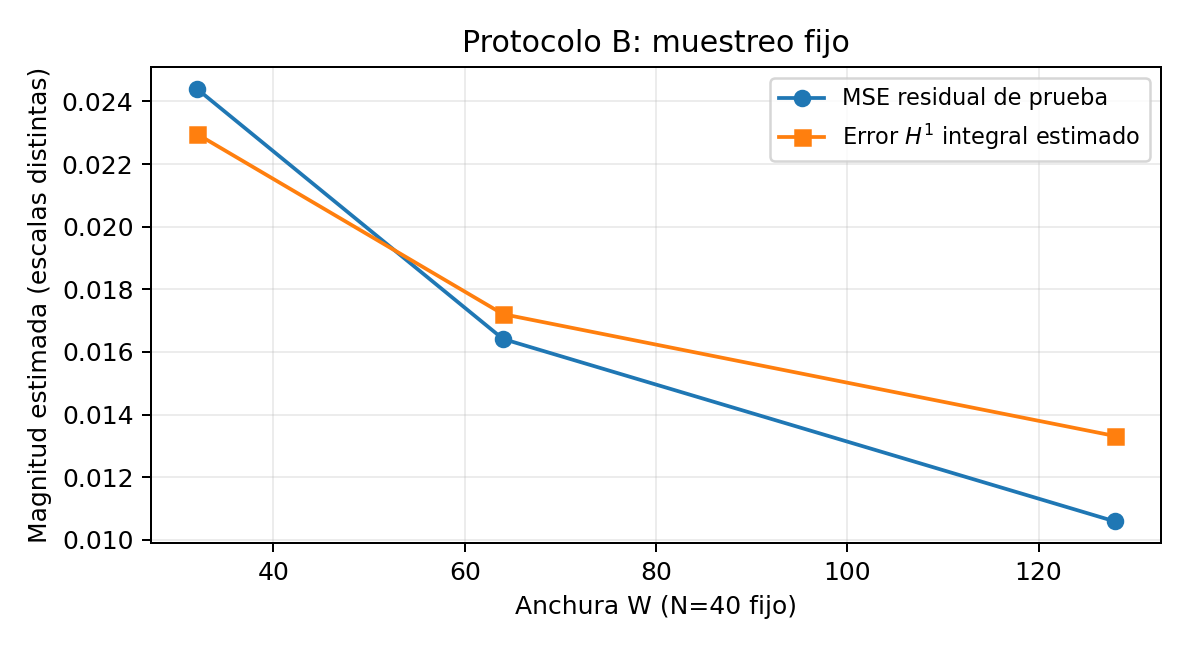
\includegraphics[width=0.82\linewidth]{imagenes/abc_B_anchuras.png}
\caption{Protocolo B con muestreo fijo: disminución de la MSE de prueba y del error integral $H^1$ estimado. Las magnitudes tienen definiciones diferentes; se presentan en los mismos ejes únicamente para mostrar sus tendencias.}
\label{fig:abc_B}
\end{figure}

\subsection{Protocolo C: escalamiento conjunto de puntos y anchura}

En C se consideraron los pares $(m_r,W)=(1521,64)$,
$(5476,128)$ y $(11881,192)$. La primera configuración reutiliza
\emph{exactamente} el entrenamiento B de $W=64$ y no se cuenta como
una nueva muestra independiente. Se conservaron dos semillas
por configuración. En la Tabla~\ref{tab:abc_escalamiento}
se muestran las medianas observadas.

\begin{table}[htbp]
\centering
\caption{Protocolo C: escalamiento conjunto. $\varepsilon_m$ es MSE residual empírica. La última columna es una seminorma residual estimada con 4800 pares, no una cota continua.}
\label{tab:abc_escalamiento}
\small
\begin{tabular}{rrrrrr}
\hline
$m_r$ & $W$ & $a_m^{\mathrm{int}}$ & $\varepsilon_m$ & $\varepsilon_m/a_m$ & H\"older (4800) \\
\hline
1521  & 64  & $1.232\times10^{-3}$ & 0.01645 & 13.35 & 2.312 \\
5476  & 128 & $4.714\times10^{-4}$ & 0.01355 & 28.74 & 2.053 \\
11881 & 192 & $2.637\times10^{-4}$ & 0.00890 & 33.76 & 1.943 \\
\hline
\end{tabular}
\end{table}

\begin{figure}[htbp]
\centering
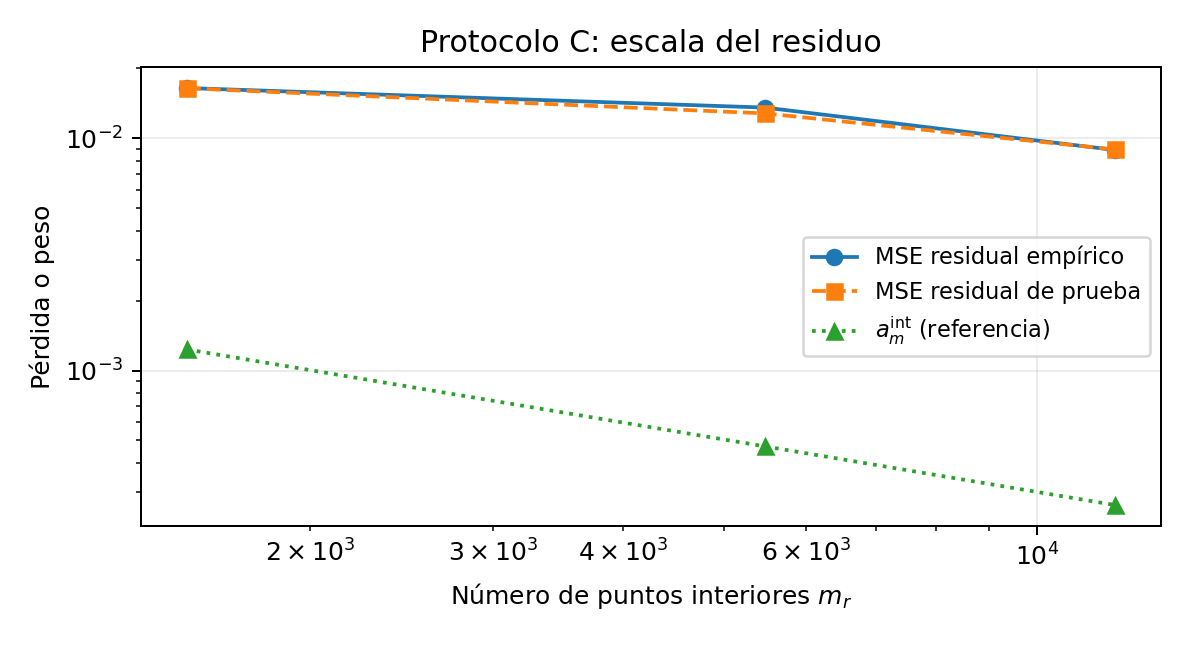
\includegraphics[width=0.77\linewidth]{imagenes/abc_C_escala.png}
\caption{Protocolo C: pérdidas residuales de entrenamiento y prueba en comparación con la escala teórica $a_m^{\mathrm{int}}$. El peso es una referencia analítica, no una curva ajustada a las pérdidas.}
\label{fig:abc_C_escala}
\end{figure}

\begin{figure}[htbp]
\centering
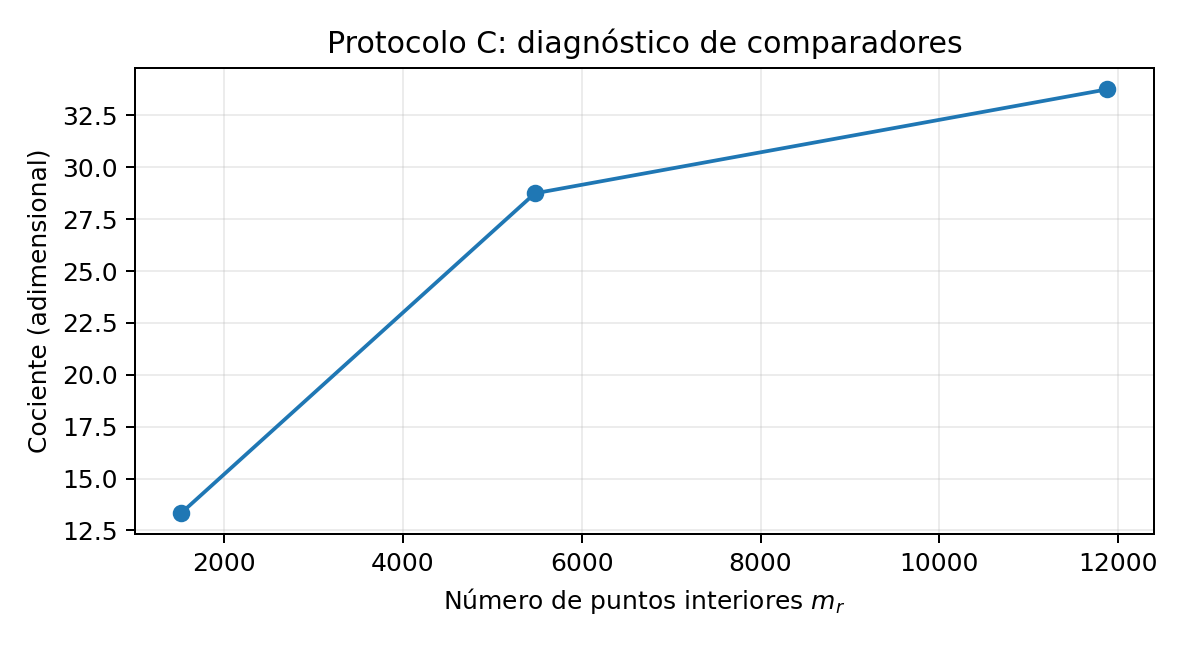
\includegraphics[width=0.77\linewidth]{imagenes/abc_C_cociente.png}
\caption{Cociente $\varepsilon_m/a_m^{\mathrm{int}}$ del protocolo C. Su crecimiento en las tres configuraciones no respalda todavía una cota uniforme para los comparadores entrenados.}
\label{fig:abc_C_cociente}
\end{figure}

El ajuste log--log \emph{puramente descriptivo y condicionado al
presupuesto fijo de optimización} de las tres medianas da
\[
 \varepsilon_m^{\mathrm{obs}} \propto m_r^{-0.284},
\]
frente a la escala suficiente $a_m^{\mathrm{int}}\asymp m_r^{-0.750}$.
Este contraste no estima una tasa intrínseca de aproximación de la
familia $\tanh$: en C también cambia la anchura y el entrenamiento
consta de 900 pasos Adam con lotes de 128 puntos y cuatro etapas
L--BFGS que utilizan subconjuntos de solo 512 puntos. Esos 512
puntos representan respectivamente 33.7\%, 9.3\% y 4.3\% de las
tres muestras interiores. Por tanto, el presupuesto efectivo de L--BFGS
cubre una fracción decreciente del conjunto de colocación. El primer
caso C reproduce B, no es una repetición independiente. Con tres
tamaños y dos semillas no se identifica una tasa asintótica ni se
demuestra que la condición falle para toda sucesión de redes.

La inspección con $1200$ y $4800$ pares muestra valores discretos
moderados del residuo, pero las estimaciones no son iguales.
La Figura~\ref{fig:abc_C_holder} permite apreciar la sensibilidad
a la densidad de evaluación; aumentar el número de pares no produce
por sí mismo una cota superior certificada.

\begin{figure}[htbp]
\centering
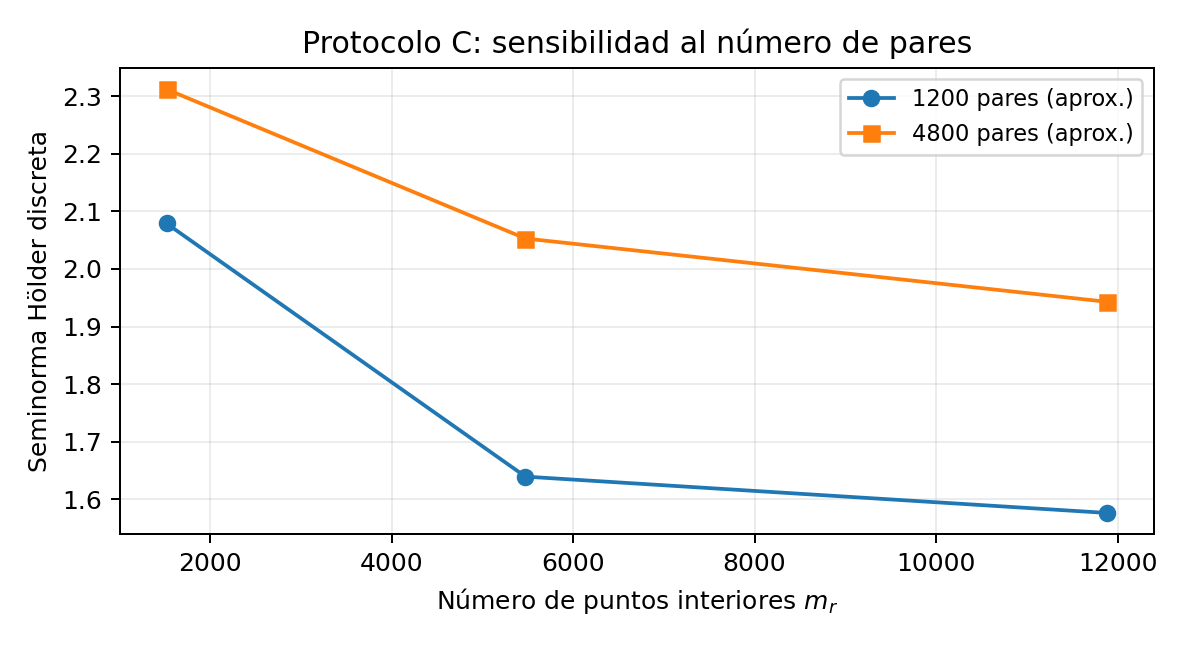
\includegraphics[width=0.77\linewidth]{imagenes/abc_C_holder_pares.png}
\caption{Estimaciones discretas de regularidad residual con dos presupuestos de pares. El supremo continuo no se calcula.}
\label{fig:abc_C_holder}
\end{figure}

\paragraph{Interpretación matemática.}
Los protocolos A--C respaldan que el refinamiento de la optimización
y el aumento de anchura, bajo las configuraciones ensayadas, reducen
los errores de prueba. Los valores discretos de regularidad no
presentan un crecimiento sistemático en el escalamiento C. Sin
embargo, la condición suficiente de la
Sección~\ref{sec:comparadores_aproximados} exige simultáneamente
control continuo de seminormas y una pérdida de comparador con
$\varepsilon_m=O(a_m)$; si se pretende extender la conclusión a
minimizadores aproximados, también una brecha
$\delta_m=O(a_m)$. El experimento no certifica ninguna de estas
propiedades asintóticas, ni la minimización global por Adam o L--BFGS.
El uso de muestras de entrenamiento aleatorias aproxima el protocolo
de muestreo de la teoría, pero no reemplaza la demostración probabilística.

\section{Comparación: elementos finitos (FEM), volúmenes finitos (FVM) y PINNs}
\label{sec:comparacion}

Finalmente, se realizó un estudio comparativo resolviendo la misma EDP de Poisson 2D utilizando tres enfoques numéricos distintos:
\begin{enumerate}
    \item \textbf{FEM:} Implementado mediante la librería \texttt{scikit-fem}~\cite{gustafsson2020scikitfem}.
    \item \textbf{FVM:} Implementado mediante la librería \texttt{FiPy}~\cite{guyer2009fipy}.
    \item \textbf{PINN:} Nuestra implementación en PyTorch~\cite{paszke2019pytorch}.
\end{enumerate}
El script comparativo itera sobre resoluciones de discretización para FEM/FVM y cantidades de puntos de colocación para la PINN. Estas cantidades no representan el mismo costo computacional; por ello, la gráfica debe entenderse como una comparación de error frente al parámetro de refinamiento de cada método, no como una comparación costo--precisión. El código del Apéndice A y el cuaderno computacional permiten reconstruir las tablas y figuras a partir de los solvers y entrenamientos registrados; los archivos de resultados conservados facilitan su trazabilidad. En esta comparación la PINN se resuelve con entrenamiento finito, de modo que la precisión observada depende del optimizador y de la semilla.

El barrido se ejecutó para $N\in\{10,20,30,40,60,80\}$; cada error se calculó sobre una cuadrícula común de $10\,201$ puntos. La PINN se entrenó durante $4\,000$ épocas por resolución, con distinta semilla en cada valor de $N$. La tabla permite cuantificar el comportamiento que se observa en la figura.

\begin{table}[htbp]
\centering
\caption{Errores relativos $L^2$ de los tres métodos en Poisson 2D.}
\label{tab:comparacion_fem_fvm}
\small
\begin{tabular}{rccc}
\hline
$N$ & FEM & FiPy (FVM) & PINN \\
\hline
$10$ & $3.891\times10^{-2}$ & $3.872\times10^{-2}$ & $1.261\times10^{-2}$ \\
$20$ & $9.743\times10^{-3}$ & $9.708\times10^{-3}$ & $1.176\times10^{-2}$ \\
$30$ & $4.325\times10^{-3}$ & $4.323\times10^{-3}$ & $1.584\times10^{-2}$ \\
$40$ & $2.433\times10^{-3}$ & $2.432\times10^{-3}$ & $1.372\times10^{-2}$ \\
$60$ & $1.081\times10^{-3}$ & $1.081\times10^{-3}$ & $1.373\times10^{-2}$ \\
$80$ & $6.082\times10^{-4}$ & $6.082\times10^{-4}$ & $1.094\times10^{-2}$ \\
\hline
\end{tabular}
\end{table}

\begin{figure}[h!]
    \centering
    \includegraphics[width=0.9\linewidth]{imagenes/comparacion_fem_fvm_pinn_reproducida.png}
    \caption{Comparación log--log de errores relativos $L^2$ para FEM, FVM y PINN en Poisson 2D, calculados sobre una cuadrícula común de evaluación. El parámetro de resolución $N$ no representa el mismo costo en los tres algoritmos.}
    \label{fig:comparison_methods}
\end{figure}

\begin{figure}[h!]
    \centering
    \includegraphics[width=0.92\linewidth]{imagenes/mapas_errores_fem_fvm_pinn.png}
    \caption{Distribución espacial del error absoluto de FEM, FiPy y PINN sobre el mismo conjunto de evaluación. La barra de colores compartida permite comparar magnitudes entre métodos.}
    \label{fig:mapas_errores_comparados}
\end{figure}

\begin{figure}[htbp]
\centering
\includegraphics[width=\linewidth]{imagenes/benchmark_mapas_error_escalas_independientes.png}
\caption{Errores puntuales para los tres métodos con escalas de color independientes. La figura permite examinar la estructura espacial de errores pequeños, pero no sirve para comparar magnitudes por color entre paneles; esa comparación corresponde a la Figura~\ref{fig:mapas_errores_comparados}.}
\label{fig:mapas_errores_escalas_independientes}
\end{figure}

\begin{figure}[htbp]
\centering
\includegraphics[width=0.86\linewidth]{imagenes/benchmark_poisson2d_error_vs_tiempo.png}
\caption{Error relativo $L^2$ frente a tiempo registrado para FEM, FVM y la PINN de referencia. Los tiempos corresponden a implementaciones y rutas de cómputo diferentes, no a un presupuesto igualado de recursos.}
\label{fig:comparacion_error_tiempo}
\end{figure}


\subsection*{Discusión comparativa}
\begin{itemize}
  \item \textbf{Exactitud.} FEM y FVM exhiben una disminución muy regular del error al refinar la discretización, aproximadamente proporcional a $N^{-2}$ en el rango estudiado. En la ejecución $N=10$ la PINN registra el menor error de los tres métodos, pero una sola semilla no autoriza atribuir una ventaja sistemática a la formulación. El error PINN oscila, en parte porque la semilla de entrenamiento cambia con $N$.
  \item \textbf{Costo.} Para $N=80$ se registraron $3.12$ s (FEM), $0.076$ s (FVM) y $23.68$ s (PINN) en las implementaciones utilizadas. Son tiempos de la ejecución concreta, no una comparación normalizada de hardware ni de costo de obtención de una misma exactitud: la PINN usó aceleración CUDA y los solvers clásicos siguieron rutas distintas de cómputo.
  \item \textbf{Comparabilidad.} El número de celdas, los grados de libertad de FEM/FVM, los parámetros de la red y las evaluaciones del residuo son recursos diferentes. Una comparación costo--precisión completa debe reportar tiempo de pared, memoria y número de parámetros o grados de libertad.
  \item \textbf{Integración de datos.} La PINN incorpora observaciones mediante un término adicional de pérdida. Esta es una diferencia de formulación útil, pero el capítulo no compara problemas inversos ni métodos clásicos de asimilación de datos.
\end{itemize}

\section*{Conclusión del capítulo}

Los ejemplos de regresión, crecimiento logístico y Poisson 1D permiten seguir el tránsito desde el ajuste de una red hasta la minimización de residuos diferenciales. La separación de componentes de pérdida identifica restricciones dominantes durante el entrenamiento, pero no equivale a una separación del error de solución. La comparación exploratoria de regularizadores 1D no permite derivar tasas asintóticas.

La reproducción bibliográfica con Dirichlet débil para $u^*(x)=\tanh(x)$ muestra una reducción cualitativa del error al ampliar la muestra. El segundo problema, con solución altamente oscilatoria y Dirichlet fuerte, no reproduce la tendencia decreciente publicada. Una revisión de la función objetivo corrigió el peso regularizador y un diagnóstico posterior mostró respuestas distintas al uso de minilotes en PINN y LIPR. La causa de la discrepancia no se reduce a un solo elemento de protocolo y sigue abierta.

El diagnóstico H\"older ilustra la importancia de la regularidad del operador y la cobertura de los puntos de colocación, pero sus máximos discretos no constituyen certificados del supremo continuo. En dos dimensiones, la evaluación conjunta de los residuos y errores en una malla independiente aporta evidencia sobre la separación entre pérdida empírica y comportamiento fuera de la muestra. En particular, con Dirichlet fuerte y $N=12$, la pérdida residual media cuadrática de prueba supera en torno a $576$ veces a la de entrenamiento.

El barrido principal de Poisson 2D comprende cuatro resoluciones, tres semillas y dos tratamientos de frontera. La parametrización fuerte produjo, en $N=75$, una mediana del error relativo $L^2$ unas $35.6$ veces menor que la versión penalizada, y un error relativo $H^1$ unas $25.7$ veces menor. El menor error requirió mayor tiempo de entrenamiento y mostró estabilización en las resoluciones más altas. Estos resultados constituyen evidencia computacional en un régimen finito, no una prueba de las hipótesis de convergencia asintótica del Capítulo~\ref{chap:convergencia}.

El estudio de comparadores aproximados con redes $\tanh$ distingue optimización, anchura y escalamiento de muestreo. En el protocolo C, la MSE residual disminuye mientras el cociente $\varepsilon_m/a_m^{\mathrm{int}}$ crece entre las tres escalas consideradas. En consecuencia, las observaciones no verifican la tasa suficiente del Capítulo~\ref{chap:convergencia}; tampoco la contradicen como afirmación asintótica bajo hipótesis adicionales.

En la comparación exploratoria de FEM, FVM y PINN, los métodos clásicos presentan un error que decrece de modo regular bajo refinamiento. El entrenamiento PINN del benchmark original no tiene un presupuesto ni un número de semillas que permitan juicios generales de superioridad. Las figuras con escalas comunes e independientes distinguen comparación de magnitudes de inspección espacial, mientras que la figura error--tiempo documenta únicamente el costo observado en el entorno registrado.


\chapter{Conclusiones y trabajo futuro}
\label{chap:conclusiones}

\section{Conclusiones principales}

\subsection{Conclusiones teóricas}

\begin{enumerate}
\item \textbf{Regularidad de las aproximaciones neuronales.} Bajo las condiciones de suavidad de la activación y control de parámetros empleadas en el Capítulo~\ref{chap:convergencia}, las redes permiten definir clásicamente los residuos de operadores elípticos de segundo orden. El control de sus seminormas no es automático: forma parte de las hipótesis de los resultados de convergencia.

\item \textbf{De la pérdida empírica a la continua.} El argumento de cobertura asociado al trabajo de Shin, Darbon y Karniadakis~\cite{shin2020convergence} explica por qué minimizar un residuo sobre muestras finitas no basta sin condiciones adicionales de muestreo y regularidad H\"older. La reconstrucción de las estimaciones muestra dónde intervienen las probabilidades de cobertura, los pesos de regularización y las constantes del dominio.

\item \textbf{Del residuo integral al uniforme.} El control H\"older limita la posibilidad de que los residuos se concentren en regiones no detectadas por las muestras. El paso de pérdidas integrales a normas uniformes se obtiene bajo las cotas de regularidad establecidas, no como consecuencia directa del comportamiento del optimizador.

\item \textbf{Comparadores y minimizadores aproximados.} Como extensión cuantitativa de la reconstrucción de Shin, la Sección~\ref{sec:comparadores_aproximados} reemplaza la interpolación empírica exactamente nula por comparadores con pérdida $\varepsilon_m$ y minimizadores con brecha de suboptimalidad $\delta_m$. La condición suficiente $\varepsilon_m+\delta_m=O(a_m)$, donde $a_m$ es el peso regularizador, preserva el control uniforme de las seminormas y las tasas condicionales. No se demuestra que las redes concretas ni los entrenamientos numéricos satisfagan esa condición.

\item \textbf{Estabilidad elíptica y error de aproximación.} Una vez controlados el residuo y el defecto de frontera, las estimaciones elípticas permiten acotar el error de la solución. En Poisson con Dirichlet fuerte resulta natural la estimación energética en $H^1$. Estas conclusiones son condicionales y se apoyan en el marco de Shin y la teoría elíptica clásica~\cite{gilbarg2001elliptic}. No se demuestra que un entrenamiento finito alcance necesariamente los minimizadores globales ni que las arquitecturas fijas utilizadas satisfagan las hipótesis de aproximación exacta.
\end{enumerate}

\subsection{Conclusiones computacionales}

Los ejemplos introductorios muestran la diferencia entre optimizar componentes de la función de pérdida y medir el error de la solución respecto de una referencia. En Poisson 1D, la comparación de la PINN estándar, la penalización cuadrática media y la regularización LIPR presenta descensos de error que dependen tanto del tamaño de muestra como de la escala de los términos de regularización; esos descensos no deben interpretarse por sí solos como tasas teóricas.

La reproducción del primer experimento elíptico de Shin presenta una tendencia cualitativa de reducción del error con Dirichlet penalizado. En el experimento oscilatorio, con Dirichlet impuesto exactamente, permanecen errores altos y no monótonos. La corrección posterior del peso LIPR y un ensayo controlado con y sin minilotes no explican por completo la discrepancia. El problema sigue siendo una limitación de reproducibilidad y optimización, no un contraejemplo a resultados asintóticos formulados bajo supuestos más fuertes. Las dificultades conocidas de dinámica de gradientes y condicionamiento~\cite{wang2021gradient,krishnapriyan2021failure} proporcionan contexto, pero no permiten atribuir una causa única a estas ejecuciones.

El diagnóstico de la regularidad H\"older permite inspeccionar diferencias entre residuos en puntos de colocación y valores calculados sobre mallas auxiliares. Sus seminormas y máximos son evaluaciones finitas y no cotas certificadas de los supremos continuos. La distinción reaparece en Poisson 2D: al evaluar los modelos sobre una malla de $201\times201$ puntos, es posible registrar conjuntamente pérdida residual de prueba, residuo máximo evaluado, error máximo y defecto de Dirichlet. La desigualdad del principio del máximo ofrece el marco interpretativo, sin convertir los máximos discretos en una comprobación rigurosa de dicha desigualdad para todo el dominio.

El nuevo barrido de Poisson 2D comprende $24$ ejecuciones: cuatro resoluciones, tres semillas y dos tratamientos de frontera. La imposición fuerte
\[
  h_\theta(x,y)=(1-x^2)(1-y^2)N_\theta(x,y)
\]
produce errores relativos $L^2$ y $H^1$ sustancialmente menores que la penalización de frontera en las configuraciones estudiadas. Para $N=75$, las medianas $L^2$ son $1.737\times10^{-4}$ con Dirichlet fuerte y $6.187\times10^{-3}$ con Dirichlet penalizado; las medianas $H^1$ son $5.483\times10^{-4}$ y $1.408\times10^{-2}$, respectivamente. Esta diferencia se obtiene con mayor tiempo computacional en el caso fuerte. La estabilización de errores en las mayores resoluciones impide hablar de una tasa asintótica observada para toda la familia.

Los resultados revelan asimismo una separación significativa entre pérdidas residuales evaluadas sobre los puntos de colocación y sobre la malla independiente: para $N=12$ y Dirichlet fuerte, las medianas respectivas son $1.816\times10^{-4}$ y $1.045\times10^{-1}$. Este hallazgo es coherente con la función de las hipótesis de cobertura y regularidad de la teoría, sin representar su verificación experimental completa.

El estudio complementario de redes $\tanh$ con Dirichlet fuerte
(Sección~\ref{sec:experimentos_tanh_abc}) distinguió continuación de
L--BFGS (A), comparación de anchuras a muestreo fijo (B) y escalamiento
conjunto (C). En B, la mediana del error residual de prueba pasó de
$0.02440$ a $0.01059$ al aumentar $W$ de $32$ a $128$. En C, con
$m_r=1521,5476,11881$, la pérdida empírica disminuyó, pero la razón
$\varepsilon_m/a_m^{\mathrm{int}}$ creció aproximadamente de $13.35$ a
$33.76$. La pendiente descriptiva $-0.284$ de las tres medianas, obtenida con
un presupuesto fijo de 900 pasos Adam y etapas L--BFGS sobre 512
puntos, es menos pronunciada que el exponente $-0.750$ del criterio
suficiente. No constituye una estimación de la tasa asintótica de
aproximación de las clases neuronales.
Por tanto, el protocolo aporta evidencia de mejor aproximación y de
regularidad residual moderada en evaluaciones discretas, pero no
verifica la condición asintótica de comparadores aproximados.

La comparación FEM/FVM/PINN muestra que, dentro de los regímenes computados, FEM y FVM reducen sus errores de forma regular al refinar la discretización, mientras que la PINN del benchmark presenta variaciones por resolución e inicialización. Los costos registrados en CPU y GPU describen esas implementaciones concretas; no representan igualdad de recursos ni una comparación general de eficiencia. El experimento adicional de Dirichlet fuerte muestra, por otra parte, que el comportamiento de una PINN depende de manera importante de su parametrización de frontera y del protocolo de optimización.

\section{Limitaciones del estudio}

\begin{itemize}
\item Las hipótesis teóricas sobre minimizadores globales, regularidad H\"older y existencia de aproximaciones exactas o suficientemente controladas no quedan garantizadas por Adam y L--BFGS. La Hipótesis 2 del marco de Shin exige condiciones restrictivas sobre las clases neuronales; la extensión con comparadores aproximados reduce la exigencia de interpolación exacta, pero requiere una tasa cuantitativa de aproximación y suboptimalidad que los experimentos no certifican.
\item Parte de las reproducciones emplea puntos equiespaciados, mientras que los resultados probabilísticos se apoyan en hipótesis de muestreo que no son equivalentes. Una malla de evaluación densa tampoco certifica normas uniformes continuas.
\item La revisión de la función objetivo LIPR corrigió el peso de regularización para que dependa de $N_f$ total. Cuando se usan minilotes, la estimación del máximo de derivadas sigue siendo un sustituto del funcional sobre toda la muestra.
\item El problema oscilatorio de Shin no reprodujo su tendencia de error. El diagnóstico controlado tiene una semilla y un presupuesto limitado; se desconocen las contribuciones relativas de inicialización, frecuencia, cobertura y optimización.
\item En A--C se minimizó el residuo cuadrático, pero no la pérdida
regularizada con seminorma H\"older del Teorema~2. Por tanto, se
estudiaron posibles comparadores empíricos y no minimizadores
comprobados de aquella función objetivo; ni la suboptimalidad global
$\delta_m$ ni la tasa de aproximación para todas las muestras quedan
verificadas.
\item El estudio A--C de redes $\tanh$ tiene solo dos semillas por
configuración y tres escalas en el protocolo C; el primer punto C
reutiliza B y no es una repetición independiente. Las seminormas
residuales provienen de pares finitos. Los checkpoints históricos son
necesarios para reproducir A; las tablas agregadas no reemplazan los
archivos por semilla, el historial o una cota de suboptimalidad global.
\item El barrido 2D utiliza tres semillas y una arquitectura base fija. Es útil para examinar el efecto del refinamiento y las condiciones de frontera, pero no separa por completo errores de aproximación y optimización ni verifica resultados asintóticos para familias crecientes de espacios neuronales.
\item La comparación FEM/FVM/PINN de referencia utiliza una única realización de PINN por resolución, diferentes algoritmos y rutas de cómputo. Sus tiempos y errores son propios del entorno utilizado y no admiten extrapolaciones generales de eficiencia.
\item La geometría cuadrada no tiene frontera global $C^{2,\alpha}$. Las estimaciones utilizadas deben justificarse mediante hipótesis adecuadas a ese dominio; no se generalizan sin análisis adicional a todas las geometrías con esquinas o interfaces.
\end{itemize}

\section{Líneas de trabajo futuro}

\begin{enumerate}
\item \textbf{Diagnóstico del caso oscilatorio.} Comparar varias semillas y presupuestos mayores, registrar el residuo fuera de muestra y controlar las diferencias entre una época, un paso de Adam y una iteración de L--BFGS, antes de formular conclusiones sobre reproducibilidad frente a Shin.
\item \textbf{Verificación de tolerancias teóricas.} Investigar condiciones de arquitectura y complejidad que garanticen comparadores con $\varepsilon_m=O(a_m)$, así como métodos para acotar la suboptimalidad $\delta_m$ de los optimizadores. Una pérdida final pequeña no constituye por sí sola una cota de suboptimalidad global.
\item \textbf{Control verificable de regularidad.} Diseñar procedimientos para obtener cotas superiores de seminormas H\"older y residuos uniformes, distinguiéndolos de evaluaciones discretas o estimadores empíricos.
\item \textbf{Muestreo y error fuera de muestra.} Explorar puntos adaptativos o aleatorios, y estudiar cómo cambian las diferencias entre pérdida empírica y pérdida residual de prueba conforme varían resolución, arquitectura y presupuesto.
\item \textbf{Contornos y geometrías.} Extender la comparación entre imposición exacta y penalizada de Dirichlet a datos de frontera no homogéneos, otros dominios y formulaciones variacionales.
\item \textbf{Comparación de costo y precisión.} Diseñar benchmarks que controlen hardware, múltiples inicializaciones, criterios de parada y tolerancias de error entre FEM, FVM y PINN, incluyendo problemas inversos y con observaciones parciales.
\end{enumerate}



%-----------------
%	BIBLIOGRAFIA
%-----------------
\bibliographystyle{ieeetr}
\bibliography{bib/biblio}


%------------
%	Anexos
%------------
\appendix
% El comando \appendix cambia la numeración a letras y el nombre a "Apéndice"

\chapter{Implementación computacional}
\label{app:codigo}
\singlespacing
\lstset{basicstyle=\ttfamily\scriptsize,breaklines=true,numbersep=4pt,frame=none}

Se presentan los programas empleados en el Capítulo~\ref{chap:resultados}. Los listados A.1--A.12 documentan los experimentos iniciales del proyecto; el A.8 presenta ahora el código corregido para nuevas ejecuciones, mientras que el archivo histórico original se conserva aparte para la trazabilidad de los CSV publicados. Los experimentos adicionales y las correcciones del protocolo se reproducen en el cuaderno incluido en \texttt{cuadernos/}; las secciones añadidas al final de este apéndice detallan su procedencia y los archivos necesarios. Los métodos comparten la ecuación de Poisson cuando corresponde, pero las nuevas celdas deben ejecutarse después de las definiciones indicadas en el cuaderno.

El cuaderno computacional se encuentra en el
\href{https://github.com/MichaelMobius/tesispucp}{repositorio público \texttt{tesispucp} de GitHub}.
Los resultados originales y los nuevos registros de ejecución se conservan por separado. El barrido 2D adicional utilizó el perfil \texttt{experimento}, mientras que la reproducción principal de Shin empleó el perfil \texttt{articulo}. El código diferencia los errores relativos
computados en los ejemplos propios de los errores RMS discretos no relativos
utilizados para contrastar las figuras del artículo de
Shin et al.~\cite{shin2020convergence}.

\noindent\textbf{Dependencias.} Python 3, PyTorch~\cite{paszke2019pytorch}, NumPy, SciPy, Matplotlib y pandas;
para la comparación con métodos clásicos, también \texttt{scikit-fem}~\cite{gustafsson2020scikitfem} y
\texttt{FiPy}~\cite{guyer2009fipy}. La precisión doble se usa en las reproducciones de Shin y
en la comparación de regularizaciones; los ejemplos iniciales emplean,
según su configuración, precisión simple.

\section{Regresión simple}
\label{app:experimento1}
\lstinputlisting[language=Python,caption={Regresión con red neuronal simple},label={lst:anexo1}]{codigos/A01_regresion.py}

\section{Ecuación logística}
\label{app:experimento2}
\lstinputlisting[language=Python,caption={PINN para la ecuación logística},label={lst:anexo2}]{codigos/A02_logistica.py}

\section{Poisson 1D con observaciones: solución seno}
\label{app:experimento3}
\lstinputlisting[language=Python,caption={Poisson 1D con datos: solución seno},label={lst:anexo3}]{codigos/A03_poisson1d_seno_datos.py}

\section{Poisson 1D con observaciones: tangente hiperbólica}
\label{app:experimento4}
\lstinputlisting[language=Python,caption={Poisson 1D con datos: tangente hiperbólica},label={lst:anexo4}]{codigos/A04_poisson1d_tanh_datos.py}

\section{Poisson 1D sin observaciones interiores}
\label{app:experimento5}
\lstinputlisting[language=Python,caption={Poisson 1D sin observaciones},label={lst:anexo5}]{codigos/A05_poisson1d_tanh_sin_datos.py}

\section{Comparación de regularizadores}
\label{app:experimento6}
\lstinputlisting[language=Python,caption={PINN estándar, penalización media y LIPR},label={lst:anexo6}]{codigos/A06_regularizaciones.py}

\section{Reproducción de Shin: Dirichlet débil}
\label{app:experimento7}
\lstinputlisting[language=Python,caption={Poisson 1D: reproducción de la Figura 3 de Shin},label={lst:anexo7}]{codigos/A07_shin_tanh.py}

\section{Reproducción de Shin: Dirichlet fuerte}
\label{app:experimento8}
\noindent El Listado~\ref{lst:anexo8} es una implementación corregida, destinada a \emph{ejecuciones futuras}: fija el peso LIPR mediante el total $N_f$ y escribe en un directorio separado. Los CSV históricos de la Tabla~\ref{tab:shin_diagnostico_nuevo} y de la reproducción principal \emph{no} se recalcularon con este archivo. La versión original permanece como \texttt{codigos/A08\_shin\_oscilatorio\_historico.py}, pero no se repite integralmente para evitar duplicación.
\lstinputlisting[language=Python,caption={Protocolo oscilatorio corregido para nuevas ejecuciones},label={lst:anexo8}]{codigos/A08_shin_oscilatorio.py}

\section{Regularidad Hölder y cobertura}
\label{app:experimento9}
Se estima la seminorma de H\"older a partir de una malla auxiliar finita. El máximo discreto no certifica el supremo continuo de los teoremas.

\lstinputlisting[language=Python,caption={Aproximación discreta de seminormas Hölder},label={lst:anexo9}]{codigos/A09_holder.py}

\section{Poisson 2D con observaciones}
\label{app:experimento10}
\lstinputlisting[language=Python,caption={PINN Poisson 2D con observaciones},label={lst:anexo10}]{codigos/A10_poisson2d_datos.py}

\section{Poisson 2D sin observaciones}
\label{app:experimento11}
\lstinputlisting[language=Python,caption={PINN Poisson 2D sin observaciones},label={lst:anexo11}]{codigos/A11_poisson2d_sin_datos.py}

\section{Comparación FEM, FVM y PINN}
\label{app:experimento12}
Los errores se evalúan sobre una cuadrícula común.

\lstinputlisting[language=Python,caption={Comparación numérica FEM, FVM y PINN},label={lst:anexo12}]{codigos/A12_fem_fvm_pinn.py}



\section{Datos, entorno y trazabilidad del protocolo revisado}
\label{app:protocolo_revisado}

\paragraph{Cuaderno y fuentes de datos.}
El cuaderno de Colab se adjunta al proyecto como archivo ejecutable.
Los datos numéricos utilizados para actualizar los Capítulos IV y V se adjuntan en la carpeta \texttt{resultados/}, sin sustituir los CSV históricos. Los archivos clave son:
\begin{itemize}
\item \texttt{convergencia\_poisson2d\_revisada.csv}: una fila por cada una de las $24$ ejecuciones, con número de puntos, semilla, tipo de contorno, errores, residuos, defectos de frontera, tiempos y firma de configuración;
\item \texttt{resumen\_convergencia\_poisson2d.csv}: medianas y desviaciones estándar de las tres semillas;
\item \texttt{estabilidad\_modelos\_originales\_2d.csv}: reevaluación, en una malla distinta, de los dos experimentos 2D originales;
\item \texttt{diagnostico\_oscilatorio\_controlado.csv}: comparación controlada de lote completo y minilote en el problema 1D de alta frecuencia;
\item \texttt{resultados\_shin\_oscilatorio.csv}: tabla principal de la reproducción oscilatoria con la versión de función objetivo registrada;
\item \texttt{comparacion\_fem\_fvm\_pinn.csv}: resultados del benchmark con $N=30$ y tiempos de ejecución;
\item \texttt{entorno\_revision.json}: versiones del entorno histórico; el archivo \texttt{HISTORICO\_manifiesto\_sha256.csv} es propio de otra ejecución y no certifica este depósito; \texttt{MANIFIESTO\_DEPOSITO\_SHA256.csv} es el inventario generado para los archivos que se entregan ahora.
\end{itemize}

El entorno registrado fue Python 3.13.16, PyTorch 2.11.0 con CUDA 13.0, NumPy 2.1.3, SciPy 1.16.3, FiPy 4.0.3 y scikit-fem 12.0.2, sobre una GPU NVIDIA A100-SXM4-40GB. En el barrido 2D se empleó \texttt{torch.float32} y en Shin \texttt{torch.float64}. Se adjuntan los $24$ modelos de barrido 2D en \texttt{modelos\_2d\_barrido/}, los ocho modelos de diagnóstico oscilatorio en \texttt{diagnostico\_shin\_modelos/} y los checkpoints disponibles en \texttt{checkpoints\_shin/}. No debe asumirse que un archivo de pesos histórico es intercambiable entre versiones de código con distinta función objetivo.

\paragraph{Discretización y precisión numérica.}
En las reproducciones unidimensionales de Shin, la función \texttt{linspace} genera $N_f$ nodos desde $-1$ hasta $1$ e incluye los extremos para $N_f\geq2$, y el caso $N_f=1$ utiliza el origen; por ello no todos esos puntos pertenecen al dominio abierto. En Poisson 2D, $N=75$ representa subdivisiones por eje: $(N-1)^2=5\,476$ puntos interiores y $4(N+1)=304$ entradas de frontera, con cuatro esquinas duplicadas. El peso de penalización de frontera de los experimentos 2D originales es $10$. La ejecución 2D usa derivadas automáticas segundas en precisión simple (\texttt{float32}); el protocolo unidimensional de Shin usa \texttt{float64}. Los efectos de redondeo en segunda derivada no se cuantificaron mediante un experimento de sensibilidad de precisión.

\paragraph{Definición de época y objetivo LIPR.}
En la revisión se fijó el peso $\lambda_R=N_f^{-3/2}$ a partir del tamaño total de los puntos de colocación, incluso cuando se entrena con un lote más pequeño. Cuando se utilizan minilotes, la cantidad \texttt{max} del regularizador se evalúa en el lote y no es idéntica al máximo en todo el conjunto. En este documento, \emph{actualización Adam} designa una aplicación del optimizador a un lote; no debe confundirse con una pasada completa por los $N_f$ ejemplos. El protocolo específico y sus firmas se encuentran en las celdas que generan los CSV y los checkpoints.

\paragraph{Rectas auxiliares y regularizadores discretos.}
En las figuras de Shin, la recta de pendiente $-1$ se coloca verticalmente con la mediana de los errores positivos del barrido; es una guía visual dependiente de los datos, no un ajuste estadístico de pendiente ni una tasa demostrada. Para $\alpha=1$, el máximo de la derivada del operador y la seminorma Lipschitz son equivalentes como magnitudes continuas bajo regularidad suficiente, pero los máximos discretos LIPR y H\"older se calculan en muestras diferentes. El caso $\alpha=1/2$ se evaluó, sin un entrenamiento separado.

\paragraph{Métricas en Poisson 2D.}
Para $Q$ malla de prueba y $Q_\partial$ puntos de su frontera, los valores reportados son
\begin{align*}
 J_{\mathrm{PDE,test}}&=\frac{1}{|Q|}\sum_{z\in Q}|\Delta h_\theta(z)-f(z)|^2,\\
 R_{\infty,Q}&=\max_{z\in Q}|\Delta h_\theta(z)-f(z)|,\\
 E_{\infty,Q}&=\max_{z\in Q}|h_\theta(z)-u^*(z)|,\\
 D_{\partial,Q}&=\max_{z\in Q_\partial}|h_\theta(z)-g(z)|.
\end{align*}
La columna \texttt{cota\_estabilidad\_evaluada} almacena $B_Q=R_{\infty,Q}/2+D_{\partial,Q}$. No es una cota certificada: el máximo de un residuo sobre una malla es, en general, \emph{menor o igual} que su supremo continuo, y tampoco certifica el supremo del error. Los errores $L^2$ y $H^1$ informados se estiman discretamente y se normalizan respecto de la solución analítica.

\paragraph{Extracción de implementaciones.}
Para facilitar la auditoría sin duplicar todo el cuaderno, los siguientes listados corresponden a sus celdas de revisión. Se ejecutan dentro del cuaderno después de sus definiciones anteriores, y no constituyen programas independientes.
\lstinputlisting[language=Python,caption={Dirichlet fuerte y métricas discretas de estabilidad: extracto del cuaderno},label={lst:anexo13}]{codigos/A13_metricas_estabilidad_2d.py}
\lstinputlisting[language=Python,caption={Entrenamiento revisado y registro reproducible del barrido 2D: extracto del cuaderno},label={lst:anexo14}]{codigos/A14_barrido_dirichlet_2d.py}
\lstinputlisting[language=Python,caption={Diagnóstico controlado del caso oscilatorio: extracto del cuaderno},label={lst:anexo15}]{codigos/A15_diagnostico_oscilatorio.py}

\paragraph{Reproducibilidad y limitaciones.}
Los valores presentados se refieren a la ejecución registrada, no a una certificación matemática. Los cambios de precisión numérica, biblioteca, plataforma, semilla o función objetivo pueden modificar los resultados. La combinación de CSV, gráficos, parámetros, checkpoints y cuaderno permite inspeccionar las correspondencias entre datos y figuras; para verificar un número específico se debe ejecutar la celda correspondiente con su configuración completa y comparar la huella del archivo exportado.


\section{Protocolo de comprobaci\'on de los comparadores aproximados (A--C)}
\label{app:tanh_abc}

El cuaderno ejecutable y la nota de procedencia se adjuntan al
directorio de reproducibilidad. Las medianas reportadas est\'an
en un CSV de la carpeta de resultados; su nombre y las reglas
de interpretaci\'on, figura en la nota de procedencia. Las figuras
del estudio se reconstruyeron a partir de las medianas reportadas,
no de registros individuales inventados.

El depósito incluye el CSV individual recuperado del Colab (16 filas),
el resumen original, el entorno y las cuatro fuentes de checkpoints del
protocolo A. Los archivos originales de Drive permiten contrastar los
resultados por semilla; los modelos finales y los historiales por etapa
no se han incorporado íntegramente a esta copia. Para una auditoría de
los entrenamientos finales debe consultarse el archivo original en
Google Drive, identificado en la nota de procedencia. El manifiesto
SHA-256 del depósito se genera sobre los archivos efectivamente
entregados, y el manifiesto antiguo se conserva como histórico.
 


%\renewcommand{\appendixname}{Anexo}% Descomenta si prefieres que diga "Anexo" en vez de "Apéndice"
%\chapter*{\appendixname}
\phantomsection
\end{document}

